% TODO: fix: self-conjugate matrix == self-adjoint matrix
\documentclass[a4paper,landscape,twocolumn]{article}
\usepackage[utf8]{inputenc}
\usepackage[LGR,T1]{fontenc}
\usepackage[ngerman,english]{babel}
\usepackage{amsmath}
\usepackage{amssymb}
\usepackage{amsfonts}
\usepackage{amsthm}
\usepackage{csquotes}
\usepackage{faktor}
\usepackage{fancyhdr}
\usepackage[margin=1in]{geometry}
\usepackage{imakeidx} % before hyperref
\usepackage[pdfborder={0 0 0},colorlinks=true,citecolor=red]{hyperref}
\usepackage{mathtools}
\usepackage{stmaryrd}
\usepackage{rotating}
\usepackage{bbold}
\usepackage{scalerel}
\usepackage{stackengine}

\title{Linear Algebra 2 -- Lecture Notes}
\author{Lukas Prokop}
\date{summer term 2016}

\newcommand\meta[3]{This #1 took place on #2 (#3).\par}
\newcommand\abs[1]{|\,#1\,|}
\newcommand\set[1]{\left\{#1\right\}}
\newcommand\setdef[2]{\left\{#1\,\middle|\,#2\right\}}
\newcommand\card[1]{\left|\,#1\,\right|}
\newcommand\divides[2]{#1\,\mid\,#2}
\newcommand\mathspace{\hspace{20pt}}
\newcommand\functional[1]{\left\langle{#1}\right\rangle}
\newcommand\Q{\mathbb{Q}}
\newcommand\nope{\lightning}
\newcommand\vecfour[4]{\begin{pmatrix} #1 \\ #2 \\ #3 \\ #4 \end{pmatrix}}
\newcommand{\textgreek}[1]{\begingroup\fontencoding{LGR}\selectfont#1\endgroup}
\newcommand\equalhat{\mathrel{\stackon[1.5pt]{=}{\stretchto{%
    \scalerel*[\widthof{=}]{\wedge}{\rule{1ex}{3ex}}}{0.5ex}}}}
\newcommand\pivot[1]{\overbrace{\underbrace{#1}_{}}^{}}

\theoremstyle{definition}
\newtheorem{theorem}{Theorem}
\newtheorem{defi}{Definition}
\newtheorem{ex}{Example}
\newtheorem{rem}{Remark}
\newtheorem{lemma}{Lemma}
\newtheorem{cor}{Corollary}

\DeclareMathOperator\Hom{Hom} % homomorphism
\DeclareMathOperator\End{End} % endomorphism
\DeclareMathOperator\Aut{Aut} % automorphism
\DeclareMathOperator\image{im} % image
\DeclareMathOperator\kernel{ker} % kernel
\DeclareMathOperator\rank{rank} % rank of a matrix
\DeclareMathOperator\sign{sign}
\DeclareMathOperator\ind{index}
\DeclareMathOperator\spec{spectrum}

\DeclarePairedDelimiter\norm\lVert\rVert

\setcounter{MaxMatrixCols}{20}

\pagestyle{fancy}
\fancyhf{}
\chead{\Large{\textsc{Linear Algebra II -- Lecture Notes}}}
\lfoot{\makebox[\columnwidth]{\thepage}}
\rfoot{\makebox[\columnwidth]{\number\numexpr\value{page}+1}\stepcounter{page}}
\setlength{\headheight}{18pt}

\parindent0pt
\parskip5pt

\makeindex[name={German},title={German keywords}]
\makeindex[name={English},title={English keywords}]
\twocolumn

\begin{document}
{\Huge
  As of 11th of May 2016,
  I am not attending LinAlg2
  anymore due to difficulties
  with my upcoming student exchange year
  and work on my master thesis.

  I therefore suppose this document will not be updated any more.
}
\newpage

\maketitle
\tableofcontents
\meta{lecture}{29th of Feb 2016}{Prof. Franz Lehner}

Exam: written and orally

Tutorial session:
\begin{itemize}
  \item Every Monday, 18:30-20:00, SR~11.34
  \item Contact: \href{mailto:gernot.holler@edu.uni-graz.at}{gernot.holler@edu.uni-graz.at}
\end{itemize}
Konversatorium:
\begin{itemize}
  \item Every Monday, 10:00--10:45, SR~11.33
\end{itemize}

Topics, wie already discussed:
\begin{itemize}
  \item Vector spaces
  \item Linear maps and their equivalence with matrices
  \item We introduced equivalence of matrices ($PAQ = B$)
  \item We defined the following techniques:
    \begin{itemize}
      \item Rank
      \item Linear equation system
      \item Inverse matrices
      \item Basis transformation
    \end{itemize}
\end{itemize}

In this semester, we will discuss:
\begin{itemize}
  \item
    $PAP^{-1}$, which is related to eigenvalues and diagonalization,
    hence $\bigvee_{P}^? PAP^{-1} = D$.
\end{itemize}

\clearpage
\section{Linear maps (cont.)}

\subsection[Addition to chapter 5.2.4]{Addition to chapter 5.2.4}

\index[English]{Dual space of a vector space}
\index[German]{\foreignlanguage{ngerman}{Dualraum des Vektorraums}}
\index[English]{Linear forms}
\index[German]{\foreignlanguage{ngerman}{Linearformen}}
\index[English]{Linear functionals}
\index[German]{\foreignlanguage{ngerman}{Lineare Funktionale}}
%
$\Hom(V,W)$ in special case $W = \mathbb K$. We define,
\[ V^* \coloneqq \Hom(V,\mathbb K) \]
also denoted $V'$ is called \emph{dual space} of vector space $V$.
The elements $v* \in V*$ are called \emph{linear forms} or \emph{linear functionals}.

We denote,
\[ v^*(v) \eqqcolon \functional{v*,v} \]

\subsection{Example}
\[ V = \mathbb K^n \]
$v^*: V \to \mathbb K$ is uniquely defined with values $v^*(e_i) \eqqcolon a_i$.
\[ \functional{v^*,v} = \functional{v^*, \sum_{i=1}^n v_i e_i} = \sum_{i=1}^n v_i \functional{v^*,e_i} \]
\[ v^*\left(\sum_{i=1}^n v_i e_i\right) = \sum_{i=1}^n v_i v^*(e_i) = \sum_{i=1}^n a_i v_i \]

\subsection{More general}
%
\index[English]{Dual basis of a vector space}
\index[German]{\foreignlanguage{ngerman}{Dualbasis eines Vektorraums}}
%
We know, $\dim{\Hom(V,W)} = \dim{V} \cdot \dim{W}$.
\begin{theorem}
  \label{5.26}
  Let $V$ be a vector space over $\mathbb K$.
  \begin{itemize}
    \item $\dim{V} \eqqcolon n < \infty \Rightarrow \dim{V^*} = n$ \\
      More precisely: Let $(b_1, \ldots, b_n)$ be a basis of $V$.
      Then \[
        b_k^*: b_i \mapsto \delta_{ik} = \begin{cases} 1 & i = k \\ 0 & \text{else} \end{cases}
      \]
      is a basis of $V^*$ and is called \emph{dual basis}.
    \item For $v^* \in V^*$ it holds that $v^* = \sum_{k=1}^n \functional{v^*, b_k} \cdot b_k^*$.
    \item If $\dim{V} = \infty, (b_i)_{i \in I}$ is a basis, then it holds that $(b^*_k)_{k \in I}$ with
      \[ \functional{b_k^*, b_i} = \delta_{ik} \]
      is \emph{not} a basis of $V^*$.
  \end{itemize}
\end{theorem}
\begin{proof}
  \begin{itemize}
    \item Special case of 5.18 \\
      $(b^*_k)$ is linear independent, hence in $\sum_{i=1}^n \lambda_i b_i^* = 0$ all $\lambda_i = 0$.
      \[
        0 = \functional{\sum_{i=1}^n \lambda_i b_i^*, b_k}
          = \sum_{i=1}^n \lambda_i \functional{\underbrace{b_i^*, b_k}_{\delta_{ik}}}
          = \lambda_k \forall k
      \]
    \item Let $v \in V$ with $v = \sum_{i=1}^n v_i b_i$. We need to show
      \begin{align*}
        \functional{v^*, v} &\stackrel{!}{=} \functional{\sum_{k=1}^n \functional{v^*,b_w} b_n^*, v} \\
        \functional{\sum_{k=1}^n \functional{v^*, b_k} b_k^*, v}
            &= \sum_{k=1}^n \functional{v^*, b_k} \functional{b_k^*, v} \\
            &= \sum_{k=1}^n \functional{v^*, b_k} \functional{b_k^*, \sum_{i=1}^n v_i b_i} \\
            &= \sum_{k=1}^n \sum_{i=1}^n \functional{v^*, b_k} \underbrace{\functional{b_k^*, b_i}}_{\delta_{ki}} \cdot v_i \\
            &= \sum_{k=1}^n \functional{v^*, b_k} \functional{v^*, b_k} \cdot v_k \\
            &= \functional{v^*, \sum_{k=1}^n v_k b_k} \\
            &= \functional{v^*, v}
      \end{align*}
    \item (To be done in the practicals)
      Consider the functional
      \[ \functional{v^*, b_i} = 1 \Rightarrow v^* \not\in L((v_i^*)_{i \in I}) \]
  \end{itemize}
\end{proof}

\subsection{Remark and a definition for bilinearity}
\index[English]{Bilinear map}
\index[German]{\foreignlanguage{ngerman}{Bilineare Abbildung}}
\index[English]{Multilinear map}
\index[German]{\foreignlanguage{ngerman}{Multilineare Abbildung}}
%
The mapping $V^* \times V \to \mathbb K$ is linear in $v$ (with fixed $v^*$)
with $(v^*, v) \mapsto \functional{v^*, v}$ is linear in $v^*$ (with fixed $v$).
Such a mapping is called \emph{bilinear}.

A mapping $F: V_1 \times \ldots \times V_n \to W$ is called \emph{multilinear} ($n$-linear)
if it is linear in every component. Formally:
\[
  F(v_1, \ldots, v_{k-1}, \lambda v'_k + \mu v''_k, v_{k+1}, \ldots, v_n)
\] \[
    = \lambda F(v_1, \ldots, v_{k-1}, v'_k, v_{k+1}, \ldots, v_n) + \mu F(v_1, \ldots, v''_k, v_{k+1}, \ldots, v_n)
\]

\subsection{Example}
\label{ex-5.28}
%
\[ V = \mathbb K[x] \text{ polynomials} \]
Basis: $\setdef{x^k}{k \in \mathbb N_0}$ and $\dim{V} = \aleph_0$

Every $v^* \in V^*$ is uniquely defined by $a_k \coloneqq \functional{v^*, x^k}$
\[ (a_k)_{k \in \mathbb N_0} \]
$V^* \cong \mathbb K[[t]]$ are the formal power series
\[ = \setdef{\sum_{k=0}^\infty a_k t^k}{a_k \in \mathbb K} \]
\[ \lambda \sum_{k=0}^\infty a_k t^k + \mu \sum_{k=0}^\infty b_k t^k = \sum_{k=0}^\infty (\lambda a_k + \mu b_k) t^k \]
(Compare with Taylor series $f(x) = \sum_{n=0}^\infty \frac{f^{(n)}(0)}{n!} x^n)$)
\[ \functional{\sum_{k=0}^\infty a_k t^k, \sum_{k=0}^n b_k x^k} \eqqcolon \sum_{k=0}^n a_k b_k \text{ is well-defined} \]
\[ \rightarrow \mathbb K[x]^* \cong \mathbb K[[t]] \]

\subsection{Example}
\label{ex-5.29}
\[ C[0,1] \text{ continuous functions} \]
Example:
\begin{ex}
\[ x \in [0,1] \qquad \delta_{x}: C[0,1] \to \mathbb R \]
\[ f \mapsto f(x) \]
\[ \functional{\delta_x, f} = f(x) \]
\[ \functional{\delta_x, f} = f(x) \]
\[ I(f) = \int_0^1 f(x) \, \text{d}x \text{ is linear} \]
\end{ex}

\[ \functional{I_g,f} = \int_0^1 f(x) g(x) \, \text{d}x \]
\[ g \in C[0,1] \text{ is fixed} \]
\[ \Rightarrow I_g \in C[0,1] \]
\[
  \functional{I_g, \lambda f_1 + \mu f_2}' = \int_0^1 (\lambda f_1(x) + \mu f_2(x)) g(x) \,\text{d}x
\] \[
  = \lambda \int_0^1 f_1(x) g(x) \,\text{d}x + \mu \int_0^1 f_2(x) g(x) \,\text{d}x
\]
This also works with non-continuous $g$ (it suffices to have $g$ integratable). (Compare with measure theory and Riesz' theorem)

Does there exist some $g$ such that $f(x) = \functional{\delta_x, f} = \int_0^1 f(t) g(t) \,\text{d}t$.
(Compare with Dirac's $\delta$ function and Schwartz/Sobder theory)

\[ V^{**} = \left(V^*\right)^* \cong V \text{ if } \dim{V} < \infty \]

\begin{lemma}
  \label{lemma-5.30}
  Let $V$ be a vector space over $\mathbb K$. It requires that $\dim{V} < \infty$ and the Axiom of Choice holds.
  \begin{itemize}
    \item $v \in V \setminus \set{0} \Leftrightarrow \bigvee_{v^* \in V^*} \functional{v^*,v} \neq 0$
    \item $\bigwedge_{v \in V} v = 0 \Leftrightarrow \bigwedge_{v^* \in V^*} \functional{v^*,v} = 0$
  \end{itemize}
\end{lemma}
\begin{proof}
  Addition $v$ to a basis $B$ of $V$:
  Define $v^* \in V^*$ by
  \[ \functional{v^*,b} = \begin{cases} 1 & b = v \\ 0 & b \neq v \end{cases} \text{ for } b \in B \]
\end{proof}

\index[English]{Bidual space}
\index[German]{\foreignlanguage{ngerman}{Bidualraum}}
\begin{theorem}
  \label{theorem-5.31}
  Let $V$ be a vector space over $\mathbb K$.
  \begin{itemize}
    \item The map $\iota: V \to V^{**} \coloneqq (V^*)^*$ is called \emph{bidual space}.
      \[ \functional{\iota(v), v^*} \coloneqq \functional{v^*,v} \]
      is linear and injective.
    \item if $\dim{V} < \infty$, then isomorphism.
  \end{itemize}
\end{theorem}
\begin{proof}
  \begin{itemize}
    \item Linearity
      \[ \iota(\lambda v + \mu w) \stackrel{!}{=} \lambda \iota(v) + \mu \iota (w) \]
      must hold in every point $v^* \in V^*$:
      \begin{align*}
        \functional{\iota(\lambda v + \mu w), v^*}
          &= \functional{v^*, \lambda v + \mu w} \\
          &= \lambda \functional{v^*,v} + \mu \functional{v^*, w} \\
          &= \lambda \functional{\iota(v), v^*} + \mu \functional{\iota(w), v^*} \\
          &= \functional{\lambda \iota(v) + \mu \iota(w), v^*}
      \end{align*}
      Is it injective?
      Let $v \in \kernel{\iota}$.
      \[ \functional{\iota(v), v^*} = 0 \quad \forall v^* \in V^* \]
      \[ \Rightarrow \functional{v^*,v} = 0 \quad \forall v^* \in V^* \]
      \[ \xRightarrow{\text{Lemma~\ref{lemma-5.30}}} v = 0 \]
    \item Follows immediately, because the dimension is equal.
  \end{itemize}
\end{proof}

\index[English]{Transposed map}
\index[German]{\foreignlanguage{ngerman}{Transponierte Abbildung}}
\begin{defi}
  \label{defi-5.32}
  Let $V,W$ be vector spaces over $\mathbb K$. $f \in \Hom(V,W)$.
  We define $f^T \in \Hom(W^*,V^*)$ using $f^T(w^*) \in V^*$ via
  \[ \functional{f^T(w^*),v} = \functional{w^*,f(v)} = w^*(f(v)) = w^* \circ f(v) \]
  \[ f^T(w^*) = w^* \circ f \text{ is linear} \Rightarrow f^T(w^*) \in V^* \]
  $V$ to $W$ (with $f$) and $W$ to $\mathbb K$ (with $w^*$).

  $f^T$ is called \emph{transposed map}.
\end{defi}

\begin{ex}
  (See practicals)
  Let $\dim{V} = n$ and $\dim{W} = m$ with $B \subseteq V$ and $C \subseteq W$ as bases
  and dual bases $B^* \subseteq V^*$ and $C^* \subseteq W^*$
  \[ \Phi_{B^*}^{C^*}(f^T) = \Phi_C^B(f)^T \quad\text{transposition of matrices} \]
\end{ex}

\meta{lecture}{2nd of March 2016}{Franz Lehner}

\section{Determinants}
%
Leibnitz~1693 ($3\times 3$ matrices) \\
Seki Takukazu~1685 (most general version) \\
Gauß~1801 (\enquote{determinant}) \\
Cayley~1845 (on matrices)

\begin{description}
  \item[$n=2$]
    \begin{align*}
      ax + by &= e \\
      cx + dy &= f
    \end{align*}
    \[
      \begin{array}{cc|c}
        a & b & e \\
        c & d & f
      \end{array}
    \]
    \begin{enumerate}
      \item Case 1: $a \neq 0$ (multiply first row $-\frac{a}{b}$ times second row)
        \[
          \begin{array}{cc}
            a & b \\
            c & d \\
          \hline
            a & b \\
            0 & d - \frac{bc}{a}
          \end{array}
        \]
        Unique solution:
        \[ d - \frac{bc}{a} \neq 0 \]

      \item Case 2: $c \neq 0$ (multiple second row $-\frac{a}{c}$ times first row)
        \[
          \begin{array}{cc}
            a & b \\
            c & d \\
          \hline
            0 & b-\frac{ad}{c} \\
            c & d
          \end{array}
        \]
        Unique solution:
        \[ b - \frac{ad}{c} \neq 0 \]
    \end{enumerate}

    This gives us
    \[ ad - bc \neq 0 \]
\end{description}

\index[English]{Determinant}
\index[German]{\foreignlanguage{ngerman}{Determinante}}
\begin{defi}
  \[ \det\begin{pmatrix} a & b \\ c & d \end{pmatrix} = ad - bc = \begin{vmatrix} a & b \\ c & d \end{vmatrix} \]
  is called \emph{determinant} of $\begin{pmatrix} a & b \\ c & d \end{pmatrix}$.
\end{defi}

\subsection{Properties of determinants}
%
\begin{itemize}
  \item The determinant is bilinear in the columns and rows.

    \[ A = \begin{pmatrix} a & b \\ c & d \end{pmatrix} = (v,w) \]
    where $v$ and $w$ are column vectors of $A$.
    \[ \det(\lambda v_1 + \mu v_2, w) = \lambda \det(v_1, w) + \mu \det(v_2, w) \]
    \[ \det(v, \lambda w_1 + \mu w_2) = \lambda \det(v, w_1) + \mu \det(v, w_2) \]

    \[
      \det(\lambda v_1 + \mu v_2, w) =
      \begin{vmatrix}
        \lambda a_1 + \mu a_2 & b \\
        \lambda c_1 + \mu c_2 & d
      \end{vmatrix}
    \] \[
      = (\lambda a_1 + \mu a_2) d - (\lambda c_1 + \mu c_2) b
    \] \[
      = \lambda (a_1 d - c_1 b) + \mu (a_2 d - c_2 b)
    \] \[
      = \lambda \begin{vmatrix} a_1 & b \\ c_1 & d \end{vmatrix}
      + \mu \begin{vmatrix} a_2 & b \\ c_2 & d \end{vmatrix}
    \]
    \[ \begin{vmatrix} a & b \\ c & d \end{vmatrix} = \begin{vmatrix} a & c \\ b & d \end{vmatrix} \]
  \item
    $\det(v,v) = 0$.
    \[ \begin{vmatrix} a & a \\ c & c \end{vmatrix} = ac - ac = 0 \]
  \item
    \[ \det\begin{pmatrix} 1 & 0 \\ 0 & 1 \end{pmatrix} = \det(e_1, e_2) = 1 \]
\end{itemize}

\begin{theorem}
  \label{satz-7.3}
  The properties 1--3 of determinants (see above) characterize the determinant.

  Let $\varphi: \mathbb K^2 \times \mathbb K^2 \to \mathbb K$
  \begin{itemize}
    \item bilinear
    \item $\bigwedge_{v \in \mathbb K^2} \varphi(v,v) = 0$
    \item $\varphi(e_1, e_2) = 1$.
      Then it holds that $\varphi = \det$.
  \end{itemize}
\end{theorem}
\begin{proof}
  To show: $\varphi(v,w) = \det(v,w) \forall v,w \in \mathbb K^2$

  \[
    v = \underbrace{a e_1 + c e_2}_{\begin{pmatrix} a \\ c \end{pmatrix}}
    \qquad
    w = \underbrace{b e_1 + d e_2}_{\begin{pmatrix} b \\ d \end{pmatrix}}
  \] \begin{align*}
    \varphi(v,w) &= \varphi(a e_1 + c e_2, b e_1 + d e_2) \\
      &= a\varphi(e_1, be_1 + de_2) + c \cdot \varphi(e_2, be_1 + de_2) \\
      &= ad \underbrace{\varphi(e_1, e_2)}_{=1} + \underbrace{ab \varphi(e_1, e_1)}_{=0} + cb \varphi(e_2, e_1) + cd \underbrace{\varphi(e_2, e_2)}_{=0}
  \end{align*}
\end{proof}

\begin{lemma}
  \label{lemma-7.4}
  From (i) bilinearity and (ii) $\bigwedge_{v \in \mathbb K^2} \varphi(v,v) = 0$ it follows that
  \[ \bigwedge_{v,w \in \mathbb K^2} \varphi(v,w) = - \varphi(w, v) \]

  \begin{align*}
    0 \overset{\text{(ii)}}{=} \varphi(v+w, v+w)
      &\overset{\text{(i)}}{=} \varphi(v,v) + \varphi(v,w) + \varphi(w,v) + \varphi(w,w) \\
      &\overset{\text{(ii)}}{=} \varphi(v,w) + \varphi(w,v)
  \end{align*}
\end{lemma}

\subsection{Geometric interpretation of the determinant}
%
Consider an area with $w$ defining its breath and $v$ its depth (hence the area spanning vectors).
Let $e_1$ and $e_2$ be the spanning vectors of a rectangle corresponding to the parallelogram.
$\det(v,w)$ is the surface of the spanned parallelogram.
The sign defines the orientation of the pair $(v, w)$.
\[ \det(e_1, e_2) = 1 \qquad \det(e_2, e_1) = -1 \]

There are surfaces where the surface is infinite if you follow a vector in some direction:
\begin{itemize}
  \item Möbius strip
  \item Klein's bottle (named after Felix~Klein)
\end{itemize}

\[ A = \abs{v} \cdot h \]

\begin{figure}[!h]
  \begin{center}
    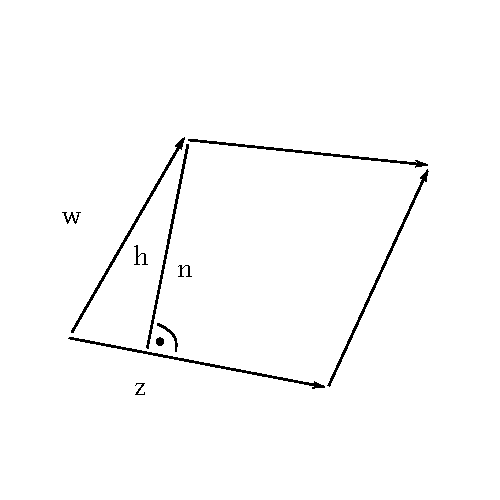
\includegraphics{img/parallelogram.pdf}
    \caption{Parallelogram}
    \label{img:para}
  \end{center}
\end{figure}

Consider Figure~\ref{img:para}.
$h$ is the length of the projection of $w$ to $v^\bot$.
\[
  v = \begin{pmatrix} a \\ b \end{pmatrix}
  \to
  \vec{n} = \begin{pmatrix} -b \\ a \end{pmatrix}
\] \[
  \langle \begin{pmatrix} c \\ d \end{pmatrix}, \begin{pmatrix} -b \\ a \end{pmatrix} \rangle
  = ad - bc
\]

\begin{proof}[Second proof]
  $A(v,w)$ satisfies properties (i)---(iii).
  \begin{itemize}
    \item Property (iii) follows immediately (the area of unit vectors in two dimensions is 1).
    \item Property (ii) follows immediately (the area of two vectors in the same direction is 0).
  \end{itemize}
  Property (i) defines the linearity in $v$
  \begin{enumerate}
    \item If $v,w$ are linear dependent, then $A(v,w) = 0$ (one is a multiple of the other)
    \item $n\in \mathbb N$ with $A(nv,w) = nA(v,w)$
    \item For $\tilde{v} = n \cdot v$:
      \[ A(\tilde{v}, w) = n \cdot A(\frac{\tilde{v}}{n}, w) \]
      \[ \Rightarrow A(\frac{\tilde{v}}{n}, w) = \frac1n A(\tilde{v}, w) \]
      \begin{align*}
        A(nv,w) &= n A(v,w) \\
        A(\frac1n v, w) &= \frac1n A(v,w) \\
        A(\frac mn v, w) &= \frac mn A(v,w) \\
        A(-v,w) &= -A(v,w)
      \end{align*}
      From continuity it follows that $A(\lambda u, w) = \lambda A(v, w)$ for $\lambda \in \mathbb R$.
      Analogously $A(v, \lambda w) = \lambda A(v, w)$.
    \item The sum is given with
      \[ A(v + w, w) = A(v, w) \]
      Compare with Figure~\ref{img:pt}, where $\operatorname{area}(2) + \operatorname{area}(3) = \operatorname{area}(2) + \operatorname{area}(1)$.
      \begin{figure}[!h]
        \begin{center}
          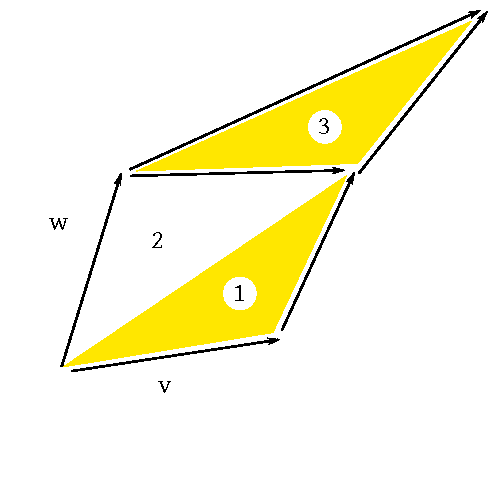
\includegraphics{img/parallelogram-translation.pdf}
          \caption{Translation of area 1 to area 3.}
          \label{img:pt}
        \end{center}
      \end{figure}
      \begin{align*}
        A(\lambda v + \mu w, w)
          &= A(\lambda v + \mu w, \frac{1}{\mu} \mu w) \\
          &= \frac1\mu A(\lambda v + \mu w, \mu w) \\
          &= \frac{1}{\mu} A(\lambda v, \mu w) \\
          &= A(\lambda v, w)
      \end{align*}

      General case: $v, w$ are linear independent and therefore basis of $\mathbb R^2$.
      Besides that, $v_1$ and $v_2$ are arbitrary.
      \begin{align*}
        v_1 &= \lambda_1 v + \mu_1 w \\
        v_2 &= \lambda_2 v + \mu_2 w
      \end{align*}
      \begin{align*}
        A(v_1 + v_2, w)
          &= A(\lambda_1 v + \mu_1 w + \lambda_2 v + \mu_2 w, w) \\
          &= A((\lambda_1 + \lambda_2) v + (\mu_1 + \mu_2) w, w) \\
          &= A((\lambda_1 + \lambda_2) v, w) \\
          &= (\lambda_1 + \lambda_2) A(v, w) \\
          &= A(\lambda_1 v, w) + A(\lambda_2 v, w)
      \end{align*}
      \[ A(\lambda_1 v + \mu_1 w, w) + A(\lambda_2 v + \mu_2 w, w) = A(v_1, w) + A(v_2, w) \]
      Additivity follows.
  \end{enumerate}
\end{proof}

\index[English]{determinant form}
\index[German]{\foreignlanguage{ngerman}{Determinantenform}}
\index[English]{Multilinearity}
\index[German]{\foreignlanguage{ngerman}{Multilinearität}}
\begin{defi}
  Let $\dim{V} = n$. A \emph{determinant form} is a map
  \[ \triangle: V^n \to \mathbb K \]
  with properties:
  \begin{enumerate}
    \item
      \[
        \bigwedge_{\lambda} \bigwedge_{k} \bigwedge_{a_1,\ldots,a_n \in V}
        \triangle (a_1, \ldots, a_{k-1}, \lambda a_k, a_{k+1}, \ldots, a_n)
        = \lambda \triangle (a_1, \ldots, a_k, \ldots, a_n)
      \]
    \item
      \[
        \bigwedge_k \bigwedge_{\substack{a_1, \ldots, a_n \\ a'_k, a''_k}}
        \triangle(a_1, \ldots, a_{k-1}, a'_k + a''_k, a_{k+1}, \ldots, a_n)
      \] \[
        \coloneqq \triangle(a_1, \ldots, a_{k-1}, a'_k + a''_k, a_{k+1}, \ldots, a_n)
      \]
    \item
      \[ \triangle(a_1, \ldots, a_n) = 0 \]
      if $\bigvee_{k \neq l} a_k = e_l$
      if $\triangle \neq 0$, i.e. $\triangle$ is non-trivial.
  \end{enumerate}
  Multilinearity is defined by the first two properties.
  Multilinearity means linearity in $a_k$ if $a_1, \ldots, a_{k-1}, a_{k+1}, \ldots, a_n$
  gets fixed.
\end{defi}

\begin{theorem}
  \label{thm-7.7}
  \[ \dim{V} = n \]
  \[ \triangle: V^n \to \mathbb K \text{ is determinant form} \]
  Then,
  \begin{enumerate}
    \item[4.]
      \[
        \bigwedge_{\lambda \in \mathbb K} \bigwedge_{i \neq j}
        \triangle(a_1, \ldots, a_{i-1}, a_{i} + \lambda a_j, a_{i+1}, \ldots, a_n)
        = \triangle(a_1, \ldots, a_i, \ldots, a_n)
      \]
      \enquote{Addition of $\lambda a_j$ to $a_i$ does not change $\triangle$}
    \item[5.]
      \[
        \bigwedge_{i>j} \triangle(a_1, \ldots, a_{j-1}, a_i, a_{j+1}, \ldots, a_{i-1}, a_j, a_{i+1}, \ldots, a_n)
      \] \[
        = -\triangle (a_1, \ldots, a_j, \ldots, a_i, \ldots, a_n)
      \]
      \enquote{Exchanging $a_i$ with $a_j$ inverts the sign}
  \end{enumerate}
\end{theorem}
\begin{proof}
  \begin{enumerate}
    \item[4.]
      \[
        \triangle(a_1, \ldots, a_i + \lambda a_j, \ldots, a_n)
      \]
      Without loss of generality: $i < j$.
      From properties 1 and 2 it follows that:
      \[
        = \triangle (a_1, \ldots, a_i, a_j, a_n)
        + \lambda \triangle(a_1, \ldots, a_j, a_j, \ldots, a_k)
      \]
      Oh, $a_j$ occurs twice! Once at index $i$ and once at index $j$.
      \[ = 0 \]
      due to property 3.
    \item[5.]
      \begin{align*}
        0 &\stackrel{\text{property~3}}= \triangle (a_1, \ldots, a_{i-1}, a_i + a_j, \ldots, a_{j-1}, a_i + a_j, \ldots, a_n) \\
          &= \triangle(a_1, \ldots, a_{i-1}, \mathbf{a_i}, \ldots, a_{j-1}, \mathbf{a_i}, \ldots, a_n) \mathbf{= 0} \\
          &+ \triangle(a_1, \ldots, a_{i-1}, \mathbf{a_i}, \ldots, a_{j-1}, \mathbf{a_j}, \ldots, a_n) \\
          &+ \triangle(a_1, \ldots, a_{i-1}, \mathbf{a_j}, \ldots, a_{j-1}, \mathbf{a_i}, \ldots, a_n) \\
          &+ \triangle(a_1, \ldots, a_{i-1}, \mathbf{a_j}, \ldots, a_{j-1}, \mathbf{a_j}, \ldots, a_n) \mathbf{= 0} \\
          &\Rightarrow \delta
      \end{align*}
  \end{enumerate}
\end{proof}

\begin{defi}
  \label{defi-7.8}
  A permutation of order $n$ is a bijective mapping $\pi: \set{1, \ldots, n} \to \set{1, \ldots, n}$.
  \[ \sigma_n = \text{ set of all permutations} \]
\end{defi}
\begin{rem}
  Notation:
  We write the elements in the first row and their images in the second row.
\end{rem}
\begin{defi}
  \label{defi-7.9}
  $\sigma_n$ constitutes (in terms of composition) a group with neutral element $\text{id}$,
  the so-called symmetric group.
\end{defi}

In the previous course (Theorem~1.40) we have proven: Compositions of bijective functions are bijective.
\begin{rem}
  For $n \geq 3$, $\sigma_n$ is non-commutative
\end{rem}
\begin{theorem}
  \label{satz-7.10}
  \[ \card{\sigma_n} = n! \]
\end{theorem}
\begin{rem}
  These are \enquote{a lot}!
\end{rem}
\begin{ex}
  \label{example-7.11}
  \[
    \begin{pmatrix}
      1 & 2 & 3 & 4 \\
      4 & 1 & 3 & 2
    \end{pmatrix} \circ \begin{pmatrix}
      1 & 2 & 3 & 4 \\
      1 & 3 & 4 & 2
    \end{pmatrix}
    = \begin{pmatrix}
      1 & 2 & 3 & 4 \\
      4 & 3 & 2 & 1
    \end{pmatrix}
  \] \[
    \begin{pmatrix}
      1 & 2 & 3 & 4 \\
      4 & 1 & 3 & 2
    \end{pmatrix}^{-1}
    = \begin{pmatrix}
      1 & 2 & 3 & 4 \\
      2 & 4 & 3 & 1
    \end{pmatrix}
  \]
\end{ex}

\index[English]{transposition}
\index[German]{\foreignlanguage{ngerman}{Vertauschung}}
\begin{defi}
  A \emph{transposition} is a permutation of the structure
  \[
    \tau = \tau_{ij}:
    \begin{array}{c}
      i \mapsto j \\
      j \mapsto i \\
      k \mapsto h
    \end{array}
    \text{ if } k \notin \set{i,j}
  \]
  Then $\tau_{ij}^{-1} = \tau_{ij}$, hence $\tau_{ij}^2 = \text{id}$.
\end{defi}
\begin{theorem}
  \label{theorem-7.13}
  $\sigma_n$ is generated by transpositions.
  With other words, every permutation $\pi$ can be represented as composition of transpositions
  \[ \pi = \tau_1 \circ \ldots \circ \tau_k \]
\end{theorem}
\begin{proof}
  \[
    \pi = \begin{pmatrix}
      1 & 2 & \ldots & n \\
      \pi(1) & \pi(2) & \ldots & \pi(n)
    \end{pmatrix}
  \]
  If $\pi = \text{id}$,
  \[ \pi = \pi \quad \tau \coloneqq \text{id} \]
  If $\pi \neq \text{id}$,
  \[ k_1 = \min\setdef{k}{k \neq \pi(k)} \]
  \begin{enumerate}
    \item
      \[ \tau_1 = \tau_{k_1 \pi(k_1)} \]
      \[
        \pi_1 = \tau_1 \circ \pi =
        \begin{pmatrix}
          1 & \ldots & \substack{k-1 \\ 1} & k_1 & \ldots \\
          1 & \ldots & \substack{k-1 \\ 1} & k_1 & \ldots
        \end{pmatrix}
      \]
      Example:
      Consider $\begin{pmatrix}
        1 & 2 & 3 & 4 & 5 & 6 & 7 \\
        1 & 3 & 5 & 4 & 7 & 6 & 2
      \end{pmatrix}$.
      \[ k_1 = 2 \]
      \[ \tau_1 = \tau_{23} \]
      \[
        \pi_1 = \tau_1 \circ \pi =
        \begin{pmatrix}
          1 & 2 & 3 & 4 & 5 & 6 & 7 \\
          1 & 2 & 5 & 4 & 7 & 6 & 3
        \end{pmatrix}
      \]
    \item
      \[ k_2 = \min\setdef{k}{k \neq \pi_1(k)} > k_1 \]
      \[ \tau_2 = \tau_{k_2,\pi(k_2)} \]
      And so on and so forth. $k_j > k_{j-1}$ ends after $\leq n$ steps.
      \[ \tau_k \circ \tau_{k-1} \circ \ldots \circ \tau_1 \circ \pi = \text{id} \]
      \[ \Rightarrow \pi = \tau_1 \circ \tau_2 \circ \ldots \circ \tau_k \]

      Regarding the example:
      \[ k_2 = 3 \]
      \[ \tau_2 = \tau_{35} \]
      \[
        \pi_2 = \tau_2 \circ \pi_1 = \tau_2 \circ \tau_1 \circ \pi =
        \begin{pmatrix}
          1 & 2 & 3 & 4 & 5 & 6 & 7 \\
          1 & 2 & 3 & 4 & 7 & 6 & 5
        \end{pmatrix}
      \]
      \[ k_3 = 5 \quad \tau_3 = \tau_{57} \]
      \[ \Rightarrow \pi = \tau_{23} \circ \tau_{35} \circ \tau_{57} \]
  \end{enumerate}
\end{proof}

\index[English]{Inversion}
\index[German]{\foreignlanguage{ngerman}{Fehlstand (Permutation)}}
\begin{defi}
  \label{def-7.14}
  An \emph{inversion} of $\pi$ is a pair $(i,j)$ such that
  $i < j$ with $\pi(i) > \pi(j)$.
  Let $F_\pi$ be the set of inversions of $\pi$.
  \[ f_{\pi} \coloneqq \card{F_\pi} \]
  \[ \operatorname{sign}(\pi) \coloneqq (-1)^{f_\pi} \eqqcolon (-1)^\pi \]
\end{defi}

\begin{ex}
  \label{example-7.15}
  \[
    \pi = \begin{pmatrix}
      1 & 2 & 3 & 4 & 5 & 6 & 7 \\
      1 & 3 & 5 & 4 & 7 & 6 & 2
    \end{pmatrix}
  \] \[
    F_\pi = \set{(2,7), (3,4), (3,7), (4,7), (5,6), (5,7), (6,7)}
  \]
  \[ f_\pi = 7 \qquad \operatorname{sign}(\pi) = -1 \]
\end{ex}

\meta{lecture}{7th of March 2016}{Franz Lehner}

\[
  \begin{vmatrix}
    a & b \\
    c & d
  \end{vmatrix}
  = ad - bc
\]

Recall: Determinant form:
\begin{enumerate}
  \item $\triangle(a_1, \ldots, \lambda a_k, \ldots, a_n) = \lambda \triangle (a_1, \ldots, a_n)$
  \item $\triangle(a_1, \ldots, a'_k + a''_k, \ldots, a_n) = \triangle(a, \ldots, a'_k, \ldots, a_n) + \triangle(a_1, \ldots, a''_k, \ldots, a_n)$
  \item $\triangle(a_1, \ldots, a_k, \ldots, a_l, \ldots, a_n) = 0$ if $a_k = a_l$
\end{enumerate}
Conclusions:
\begin{enumerate}
  \item[4.] $\triangle (a_1, \ldots, a_k + \lambda a_l, \ldots, a_n) = \triangle (a_1, \ldots, a_n)$ if $k \neq l$
  \item[5.] $\triangle (a_1, \ldots, a_k, \ldots, a_l, \ldots a_n) = -\triangle (a_1, \ldots, a_l, \ldots, a_k, \ldots a_n)$
\end{enumerate}

\[ \triangle (a_{\pi(1)}, \ldots, a_{\pi(n)}) = (-1)^k \triangle (a_1, \ldots, a_n) \]

Decompose $\pi = \tau_1 \circ \ldots \circ \tau_k \circ \tau_{12} \circ \tau_{12}$.
This decomposition is not distinct ($k$ is distinct $\mod 2$)

\[ \pi \in \sigma_n \qquad \text{permutation} \]
\[ F_\pi = \setdef{(i,j)}{i < j, \pi(i) > \pi(j), \text{ inversions }} \]
\[ f_\pi = \card{F_\pi} \]
\[ \sign(\pi) \coloneqq (-1)^{f_\pi} \eqqcolon (-1)^\pi \]

\begin{theorem}
  \label{satz-7.16}
  \begin{itemize}
    \item $\bigwedge_{\pi \in \sigma_n} \sign(\pi) = \prod_{1 \leq i < j \leq n} \frac{\pi(j) - \pi(i)}{j - i}$
    \item For transposition $\tau$ it holds that $\sign(\tau) = -1$
  \end{itemize}
\end{theorem}
\begin{proof}
  \begin{itemize}
    \item
      Every pair $\set{i,j}$ occurs in the enumerator exactly once.
      \[ \frac{\prod_{i<j} \pi(j) - \pi(i)}{\prod_{i<j} (j - i)} \]
      Denominator: $j > i$, positive.
      Enumerator: positive if $\pi(j) > \pi(i)$, negative if $\pi(i) > \pi(j)$.
    \item
      \[
        \tau =
        \begin{pmatrix}
          1 & \ldots & k & \ldots & l & \ldots & n \\
          1 & \ldots & l & \ldots & k & \ldots & n
        \end{pmatrix}
      \] \[
        F_\tau(\underbrace{(k, k + 1), (k, k + 2), \ldots, (k, l-1)}_{\text{inversions with $k$, $l-k$ times}},
        (k,l), \underbrace{(k+1, l), \ldots, (l - 1, l)}_{l-k-1 \text{ times}})
      \]
      Example:
      \[
        \begin{pmatrix}
          1 & 2 & 3 & 4 & 5 & 6 & 7 & 8 & 9 & 10 \\
          1 & 2 & 3 & 8 & 5 & 6 & 7 & 4 & 9 & 10
        \end{pmatrix}
      \]
      Yields $7$ inversions ($8$ needs to be repositioned with 3 transpositions, $4$ needs to be repositions with 4 transpositions).
  \end{itemize}
\end{proof}

\[ \sign(\pi) = \prod_{i < j} \frac{\pi(j) - \pi(i)}{j - i} \qquad {n \choose 2} \text{ factors} \]
\[ \sign(\tau) = -1 \]

\index[English]{Character}
\index[German]{\foreignlanguage{ngerman}{Charakter}}
\begin{theorem}
  \begin{enumerate}
    \item $\sign(\text{id}) = 1$
    \item $\sign(\pi \circ \sigma) = \sign(\pi) \cdot \sign(\sigma)$, hence
      \[ \sign{\sigma_n} \to (\set{+1, -1}, \cdot) \]
      is a group homomorphism.
      (In general: A group homomorphism $h: G \to (\mathcal T, \cdot)$ is called \emph{character})
    \item $\sign(\pi^{-1}) = \sign(\pi)$
  \end{enumerate}
\end{theorem}
\begin{rem}
  \[ \mathcal T = \setdef{z \in \mathbb C}{\abs{z} = 1} \]
  Torus with multiplication is a group.
  \[ \abs{z_1 \cdot z_2} = \abs{z_1} \cdot \abs{z_2} = 1 \]
\end{rem}
\begin{proof}
  \begin{enumerate}
    \item trivial
    \item
      \begin{align*}
        \sign(\pi \cdot \sigma) &= \prod_{i<j} \frac{\pi \circ \sigma(j) - \pi \circ \sigma(i)}{j - i} \\
          &= \underbrace{\prod_{i<j} \frac{\pi(\sigma(j)) - \pi(\sigma(i))}{\sigma(j) - \sigma(i)}}_{=\sign(\pi)}
             \cdot \underbrace{\prod_{i < j} \frac{\sigma(j) - \sigma(i)}{j - i}}_{\sign(\sigma)}
      \end{align*}
    \item Group homomorphism!
  \end{enumerate}
\end{proof}

\begin{cor}
  \label{cor-7.18}
  \begin{itemize}
    \item If $\pi = \tau_1 \circ \tau_2 \circ \ldots \circ \tau_k$, product of transpositions
      \[ \Rightarrow \sign(\pi) = (-1)^k \]
    \item $\mathfrak a_n \coloneqq \ker(\sign) = \setdef{\pi \in \sigma_n}{\sign(\pi) = 1}$
      \begin{center} \enquote{even permutations}, \enquote{alternating group} \end{center}
      \[ \card{\mathfrak a_n} = \frac{n!}{2} \]
  \end{itemize}
\end{cor}
\begin{cor}
  \label{cor-7.19}
  \[ \triangle: V^k \to \mathbb K \text{ determinant form} \]
  then it holds that
  \[
    \bigwedge_{\pi \in \sigma_n} \bigwedge_{a_1, \ldots, a_n \in V}
    \triangle(a_{\pi(1)}, \ldots, a_{\pi(n)}) = \sign(\pi) \cdot \triangle(a_1, \ldots, a_n)
  \]
\end{cor}
\begin{proof}
  \begin{itemize}
    \item If $\pi = \tau_{kl}$ transposition $\xrightarrow{\text{Theorem~}\ref{thm-7.7}} \triangle(a_{\tau(1)}, \ldots, a_{\pi(n)})
      = -\triangle(a_1, \ldots, a_n) = \sign(\tau_{kl}) \cdot \triangle(a_1, \ldots, a_n)$
    \item If $\pi = \tau_1 \circ \ldots \circ \tau_k = \tau_1 \circ \tilde{\pi}, \tilde{\pi} = \tau_2 \circ \ldots \circ \tau_k$
      \begin{align*}
        &\triangle(a_{\tau_1 \circ \tilde{\pi}(1)}, \ldots, a_{\tau_1 \circ \tilde{\pi}(n)}) \\
        &= -\triangle(a_{\tilde\pi(1)}, \ldots, a_{\tilde\pi(n)}) \\
        &= (-1)^2 \cdot \triangle(a_{\tilde\pi(1)}, a_{\tilde\pi(n)}) \\
        &\to (-1)^k \cdot \triangle(a_1, \ldots, a_n)
      \end{align*}
  \end{itemize}
\end{proof}
\begin{theorem}[Leibnitz' definition of $\det(A)$]
  \label{satz-7.20}
  Let $B = (b_1, \ldots, b_n)$ be the basis of $V$. $a_1, \ldots, a_n \in V$ with coordinates
  \[ \Phi_B(a_j) = \begin{bmatrix} a_{1j} \\ a_{2j} \\ \vdots \\ a_{nj} \end{bmatrix} \]
  \[ A \coloneqq [a_{ij}]_{i,j=1,\ldots,n} = \left[\Phi_B(a_1), \Phi_B(a_2), \ldots, \Phi_B(a_n)\right] \]
  Then it holds that for every determinant form $\triangle: V^k \to \mathbb K$:
  \[ \triangle(a_1, \ldots, a_n) = \det(A) \cdot \triangle(b_1, \ldots, b_n) \]
  where
  \[ \det(A) \coloneqq \sum_{\pi \in \sigma_n} \sign_{\mathbb K} \pi a_{\pi(1),1} a_{\pi(2),2} \ldots a_{\pi(n),n} \]
  is the determinant of $A$
\end{theorem}
%
\begin{ex}
  Example ($n=2$):
  \[
    \begin{vmatrix}
      a_{11} & a_{12} \\
      a_{21} & a_{22}
    \end{vmatrix}
    = a_{11} \cdot a_{22} - a_{12} \cdot a_{21}
  \]

  \[ \sign\begin{pmatrix} 1 & 2 \\ 1 & 2 \end{pmatrix} = 1 \]
  \[ \sign\begin{pmatrix} 1 & 2 \\ 2 & 1 \end{pmatrix} = -1 \]
\end{ex}
%
\begin{proof}
  \[ a_j = \sum_{j=1}^n a_{ij} b_i \]
  \begin{align*}
    \triangle(a_1, \ldots, a_n) &= \triangle\left(\sum_{i_=1}^n a_{i,1} b_i, \sum_{i_2=1}^n a_{i_2,2} b_i, \ldots, \sum_{i_n=1}^n a_{i_n,n} b_i\right) \\
      &= \sum_{i_1=1}^n a_{i,1} \sum_{i_2=1}^n a_{i_2,2} \ldots \sum_{i_n=1}^n a_{i_n,n} \underbrace{\triangle (b_i, b_{i_2}, \ldots, b_{i_n})}_{= 0 \text{ if some } i_k = i_l}
  \end{align*}
  So summands with equal indices disappear. It holds that
  $\sum_{i_1, \ldots, i_n}$ such that $i_1, \ldots, i_n$ are different.
  Hence every value from $\set{1, \ldots, n}$ occurs exactly once.
  This is the set of all permutations $\pi$ ($i_j = \pi(j)$)
  \[ = \sum_{\pi \in \sigma_n} a_{\pi(1) 1} a_{\pi(2) 2} \ldots a_{\pi(n) n} \underbrace{\triangle(b_{\pi(1)}, \ldots, b_{\pi(n)})}_{\sign(\pi) \cdot \triangle(b_1,\ldots,b_n)} \]
\end{proof}
\begin{cor}
  \label{cor-7.21}
  A determinant form is \emph{uniquely} defined on a basis ($b_1, \ldots, b_n$) by the value $\triangle(b_1, \ldots, b_n)$.
  Especially $\triangle$ is nontrivial,
  \begin{itemize}
    \item[$\Leftrightarrow$] $\triangle (b_1, \ldots, b_n) \neq 0$ on some basis.
    \item[$\Leftrightarrow$] $\triangle (b_1, \ldots, b_n) \neq 0$ in every basis $b_1, \ldots, b_n$.
  \end{itemize}

  Let $\triangle(b'_1, \ldots, b'_n) = 0$ for some other basis, represent $b_1, \ldots, b_n$ in basis $b'_1, \ldots, b'_n$
  \[ b_j = \sum a_{ij} b'_i \Rightarrow \triangle(b_1, \ldots, b_n) = \det(A) \cdot \triangle(b'_1, \ldots, b'_n) = 0 \]
  \[ \triangle(a_1, \ldots, a_n) = \det(A) \cdot \triangle(b_1, \ldots, b_n) \]
\end{cor}

\begin{theorem}
  \label{satz-7.22}
  Let $B = (b_1, \ldots, b_n)$ be a basis of $V$ over $\mathbb K$. $c \in \mathbb K$.
  For $a_1, \ldots, a_n \in V$, let $A = \left[\Phi_B(a_1), \ldots, \Phi_B(a_n)\right]$.
  Then
  \[ \triangle(a_1, \ldots, a_n) = c \cdot \det(A) \]
  defines a determinant form, specifically the unique determinant form with value
  \[ \triangle(b_1, \ldots, b_n) = c \]
\end{theorem}
\begin{proof}
  The 3 properties of a determinant form:
  \begin{enumerate}
    \item
      \begin{align*}
        \triangle(a_1, \ldots, \lambda a_k, \ldots, a_n)
        &= c \cdot \det\left[\Phi_B(a_1), \ldots, \lambda \cdot \Phi_B(a_k), \ldots, \Phi_B(a_n)\right] \\
        &= c \cdot \sum_{\pi \in \sigma_n} \sign{\pi} \cdot a_{\pi(1),1} a_{\pi(2),2} \ldots \lambda a_{\pi(k),k} \ldots a_{\pi(n),n} \\
        &= \lambda \cdot c \cdot \sum_{\pi \in \sigma_n} \sign{\pi} \cdot a_{\pi(1),1} a_{\pi(2),2} \ldots a_{\pi(n),n} \\
        &= \lambda \cdot \triangle(a_1, \ldots, a_n)
      \end{align*}
    \item
      \begin{align*}
        & \triangle(a_1, \ldots, a'_k + a''_k, \ldots, a_n) \\
          &= c \cdot \det\left[\Phi_B(a_1), \ldots, \Phi_B(a'_k) + \Phi_B(a''_k), \ldots, \Phi_B(a_n)\right] \\
          &= c \cdot \sum_{\pi \in \sigma_n} \sign{\pi} \cdot a_{\pi(1),1} \cdot a_{\pi(2),2} \cdot \ldots
             \left(a'_{\pi(k),k} + a''_{\pi(k),k}\right) \cdot \ldots \cdot a_{\pi(n),n} \\
          &= c \cdot \sum_{\pi \in \sigma_n} \sign{\pi} \cdot a_{\pi(1),1} \cdot \ldots \cdot a'_{\pi(k),k} \ldots a_{\pi(n),n} \\
          &+ c \cdot \sum_{\pi \in \sigma_n} \sign(\pi) a_{\pi(1),1} \ldots a''_{\pi(k),k} \ldots a_{\pi(n),n} \\
          &= \triangle(a_1, \ldots, a'_k, \ldots, a_n) + \triangle(a_1, \ldots, a''_k, \ldots, a_n)
      \end{align*}
    \item
      Let $a_k = a_l$ for $k < l$. Show that $\triangle(a_1, \ldots, a_n) = 0$
      \[ \tau_{kl} = \text{ transposition exchanging $k$ and $l$} \]
      \[ \sigma_n = \mathfrak a_n \dot\cup\, (\mathfrak a_n \cdot \tau_{kl}) \]
      Claim: $\setdef{\pi}{\sign{\pi} = -1} = \setdef{\pi \circ \tau_{kl}}{\sign{\pi} = +1}$
      \begin{description}
        \item[$\supseteq$] If $\sign{\pi} = +1 \Rightarrow \sign(\pi \circ \tau_{kl}) = \underbrace{\sign{\pi}}_{+1} \cdot \underbrace{\sign{\tau_{kl}}}_{-1} = -1$
        \item[$\subseteq$] If $\sign{\pi} = -1 \Rightarrow \sign(\pi \circ \tau_{kl}) = +1 \Rightarrow \pi = \underbrace{(\pi \circ \tau_{kl})}_{\in \mathfrak a_n} \circ \tau_{kl} \in \mathfrak a_n \cdot \tau_{kl}$
      \end{description}
      \begin{align*}
        \triangle(a_1, \ldots, a_n)
          &= c \cdot \sum_{\pi \in \sigma_n = \mathfrak a_n \cup \mathfrak a_n \cdot \tau_{kl}}
            \sign(\pi) a_{\pi(1),1} \ldots a_{\pi(n),n} \\
          &= \underbrace{c \cdot \sum_{\pi \in \mathfrak a_n} a_{\pi(1),1} \ldots a_{\pi(n),n}}_{\text{even}} \\
          &- \underbrace{\sum_{\pi \in \mathfrak a_n} a_{\pi \circ \tau_{kl}(1),1} \ldots a_{\pi \circ \tau_{kl}(k),k} \ldots a_{\pi \circ \tau_{ul}(l),l} \ldots a_{\pi \circ \tau_{kl}(n),n}}_{\text{odd}} \\
          &= c \cdot \sum_{\pi \in \mathfrak a_n} a_{\pi(1),1} \ldots, a_{\pi(n),n} \\
          &- \sum_{\pi \in \mathfrak a_n} a_{\pi(1),1} \ldots \underbrace{a_{\pi(l),k}}_{a_{\pi(l),l}} \ldots \underbrace{a_{\pi(k)l}}_{a_{\pi(k),k} \text{ because } a_k=a_l} \ldots a_{\pi(n),n}
      \end{align*}

      What we did:
      \begin{enumerate}
        \item $a_{\pi(l),k} = a_{\pi(l),l}$ and $a_{\pi(k),l} = a_{\pi(k),k}$ because $a_k = a_l$
        \item exchange factors
      \end{enumerate}

      \begin{align*}
        &= c \sum_{\pi \in \mathfrak a_n} a_{\pi(1),1} \ldots a_{\pi(k),k} \ldots a_{\pi(l),l} \ldots a_{\pi(n),n} \\
        &- c \sum_{\pi \in \mathfrak a_n} a_{\pi(1),1} \ldots a_{\pi(k),k} \ldots a_{\pi(l),l} \ldots a_{\pi(n),n} \\
        &= 0
      \end{align*}

      Value for $(b_1, \ldots, b_n)$
      \[ a_{ij} = \delta_{ij} \Rightarrow A = I \]
      \[ \det(I) = \sum_{\pi \in \sigma_n} \sign{\pi} \cdot \delta_{\pi(1),1} \ldots \delta_{\pi(n),n} = +1 \]
      for all $\pi(j)=j$ otherwise $0$.
      \[ \Rightarrow \pi = \text{id} \text{ is the only summand} \]
      \[ \triangle(b_1, \ldots, b_n) = \det(I) \cdot c = c \]
  \end{enumerate}
\end{proof}
\begin{rem}
  \enquote{$\mathfrak a_n$ is the subgroup of index 2}
  denoted $[\sigma_n: \mathfrak a_n] = 2$

  You might be familiar with:
  \[ \mathbb Z_n = \faktor{\mathbb Z}{n \mathbb Z} \]
  \[ [\mathbb Z : n \mathbb Z] = n \]
\end{rem}

\begin{theorem}[Summary]
  \label{summary-7.24}
  \begin{itemize}
    \item The set of determinant forms $\triangle: V^n \to \mathbb K$
      constructs a one-dimensional vector space, $\Lambda^n V$
    \item There exists a non-trivial determinant form with $\triangle(b_1,\ldots,b_n) = 1$
  \end{itemize}
\end{theorem}

\meta{lecture}{9th of March 2016}{Franz Lehner}

Revision:

\[ \triangle: V^n \to \mathbb K \]
\[ \triangle(a_1, \ldots, a_n) = \det{A} \cdot \triangle(b_1, \ldots, b_n) \]

\[ \phi_B(a_j) = \begin{pmatrix} a_{1j} \\ \vdots \\ a_{nj} \end{pmatrix} \]

\[ \det{A} = \sum_{\pi \in \sigma_n} \sign{\pi} \cdot a_{\pi(1),1} \ldots a_{\pi(n),n} \]

\[ \triangle(v_1, \ldots, v_n) \neq 0 \Leftrightarrow v_1, \ldots, v_n \text{ linear independent ($\Leftrightarrow$ basis)} \]

\begin{theorem}
  \[ \det(A \cdot B) = \det(A) \cdot \det(B) \]
\end{theorem}
\begin{lemma}
  \label{lemma-7.25}
  Let $V, W$ be vector spaces over $\mathbb K$ with $\dim{V} = \dim{W} = n$.
  \[ \triangle: W^n \to \mathbb K \]
  \[ f: V \to W \]

  \[ \Rightarrow f^n: V^n \to W^n \overset{\triangle}\to \mathbb K \]
  \[ (v_1, \ldots, v_n) \mapsto (f(v_1), \ldots, f(v_n)) \]

  Then $\triangle^f: V^n \to \mathbb K$
  \[ \triangle^f(v_1, \ldots, v_n) = \triangle(f(v_1), \ldots, f(v_n)) \]
  is a determinant form in $V$.
\end{lemma}
\begin{proof}
  \begin{enumerate}
    \item
      \begin{align*}
        \triangle f(v_1, \ldots, \lambda v_k, \ldots, v_n)
          &= \triangle(f(v_1), \ldots, f(\lambda v_k), \ldots, f(v_n)) \\
          &= \lambda \triangle(f(v_1), \ldots, f(v_n)) \\
          &= \lambda \cdot \triangle^f (v_1, \ldots, v_n)
      \end{align*}
    \item
      \begin{align*}
          &= \triangle^f (v_1, \ldots, v'_k, + v''_k, \ldots, v_n) \\
          &= \triangle(f(v_1), \ldots, f(v'_k + v''_k), \ldots, f(v_n)) \\
          &= \triangle(f(v_1), \ldots, f(v'_k) + f(v''_k), \ldots, f(v_n)) \\
          &= \triangle(f(v_1), \ldots, f(v'_k), \ldots, f(v_n)) + \triangle(f(v_1), \ldots, f(v''_k), \ldots, f(v_n)) \\
          &= \triangle^f(v_1, \ldots, v'_k, \ldots, v_n) + \triangle^f(v_1, \ldots, v_k'', \ldots, v_n)
      \end{align*}
    \item
      \begin{align*}
        \triangle^f (v_1, \ldots, v_k, \ldots, v_l, \ldots, v_n) &\qquad v_k = v_l \Rightarrow f(v_k) = f(v_l) \\
          &= \triangle(f(v_1), \ldots, f(v_k), \ldots, f(v_l), \ldots, f(v_n)) \\
          &= 0
      \end{align*}
  \end{enumerate}
\end{proof}

\begin{cor}[Conclusions for $V = W$]
  \label{cor-7.26}
  \[ \triangle: V^n \to \mathbb K \]
  non-trivial determinant form
  \[ f: V \to V \]
  \[ \Rightarrow \triangle^f \text{ is a determinant form} \]

  \[ \dim{\bigwedge^n \bigvee} = 1 \Rightarrow \bigvee_{c_f \in \mathbb K} \triangle^k = c_f \cdot \triangle \]
  \[ c_f \eqqcolon \det{f} \text{ is called determinant of $f$} \]
\end{cor}

\begin{cor}
  \label{cor-7.27}
  Let $V$, $\triangle$ and $f$ be like above.
  \begin{enumerate}
    \item
      For every basis $B = (b_1, \ldots, b_n)$
      it holds that
      \[ \triangle^f(b_1, \ldots b_n) = \triangle(f(b_1), \ldots, f(b_n)) = \det(f) \cdot \triangle(b_1, \ldots, b_n) \]
      \[ \det(f) = \frac{\triangle(f(b_1), \ldots, f(b_n))}{\triangle(b_1, \ldots, b_n)} \]
    \item
      with $a_j = f(b_j)$ it holds that
      \[ \det{\Phi_B^B(f)} = \det(f) \]
      \[ A = \Phi_B^B(f) \]
      $a_{ij} = $ i-th coordinate of $f(b_j)$ and $s_j(A) = \Phi_B(f(b_j))$.
  \end{enumerate}
\end{cor}

\begin{theorem}
  \label{theorem-7.28}
  Let $f: V \to V$ be an isomorphism $\Leftrightarrow \det(f) \neq 0$.
\end{theorem}
\begin{proof}
  Let $f$ be an isomorphism.
  \begin{align*}
    &\Leftrightarrow (f(b_1), \ldots, f(b_n)) \text{ is basis} \\
    &\Leftrightarrow \triangle (f(b_1), \ldots, f(b_n)) \neq 0 \\
    &\Leftrightarrow \det(f) \cdot \triangle(b_1, \ldots, b_n) \\
    &\Leftrightarrow \det(f) \neq 0
  \end{align*}
\end{proof}

\begin{theorem}
  \label{theorem-7.29}
  Let $f,g: V \to V$ be linear.
  \[ \Rightarrow \det(f \circ g) = \det(f) \cdot \det(g) \]
\end{theorem}
\begin{rem}
  We show: $f \circ g$ is isomorphism $\Leftrightarrow$ f and g are isomorphisms.

  If $f,g$ are invertible, then $f \circ g$ are invertible.
  \begin{enumerate}
    \item
      \[ (f \circ g)^{-1} = g^{-1} \circ f^{-1} \]
    \item
      Attention! This is wrong, if $\dim = \infty$!
      For example: $\delta: (x_1, x_2, \ldots) \mapsto (0, x_1, x_2, \ldots)$ over $\mathbb K^\infty$
      is injective, but not surjective!

      \[ S_L: (x_1, x_2, \ldots) = (x_2, x_3, \ldots) \]
      is not injective, but surjective.

      \[ S_L \circ S_R = I \]
      \[ S_R \circ S_L - I - P_1 \]

      If $f \circ g$ is bijective, then $g$ is injective and $f$ surjective.
      \[ \xRightarrow{\dim < \infty} g \text{ bijective}, f \text{ bijective} \]
  \end{enumerate}
\end{rem}
\begin{proof}
  Case distinction:
  \begin{description}
    \item[$\det(f \circ g) = 0$]
      \begin{align*}
        &\xLeftrightarrow{\text{Theorem}~\ref{theorem-7.28}} f \circ g \text{ is not bijective} \\
        &\Leftrightarrow f \text{ is not bijective or g not bijective}  \\
        &\Leftrightarrow \det(f) = 0 \lor \det(g) = 0 \\
        &\Leftrightarrow \det(f) \cdot \det(g) = 0
      \end{align*}
    \item[$\det(f \circ g) \neq 0$]
      \begin{align*}
        &\Leftrightarrow f \circ g \text{ is bijective} \\
        &\Rightarrow g \text{ bijective} \\
        &\Rightarrow \triangle^g \text{ non-trivial}
      \end{align*}
      Let $(b_1, \ldots, b_n)$ be a basis of $V$, then $\triangle$ is non-trivial determinant.
      \begin{align*}
        \det(f \circ g)
          &= \frac{\triangle(f\circ g(b_1) \ldots, f \circ g(b_n))}{\triangle (b_1, \ldots, b_n)} \\
          &= \frac{\triangle(f(g(b_1)), \ldots, f(g(b_n)))}{\triangle (g(b_1), \ldots, g(b_n))} \cdot \frac{\triangle (g(b_1), \ldots, g(b_n))}{\triangle(b_1, \ldots, b_n)} \\
          &= \frac{\triangle((b'_1), \ldots, f(b'_n))}{\triangle (b'_1, \ldots, b'_n)} \cdot \frac{\triangle (g(b_1), \ldots, g(b_n))}{\triangle(b_1, \ldots, b_n)} \\
          &= \det(f) \cdot \det(g)
      \end{align*}
      $b'_i = g(b_i)$ are also a basis, because $g$ is bijective.
  \end{description}
\end{proof}

\begin{cor}
  \label{cor-7.30}
  Let $A,B \in \mathbb K^{n\times n}$.
  \begin{enumerate}
    \item $\det(A \cdot B) = \det(A) \cdot \det(B)$
    \item $A$ is regular $\Rightarrow$ $\det(A^{-1}) = \frac{1}{\det(A)}$
    \item $\det(A) = 0 \Leftrightarrow \rank(A) < n$
    \item $\det(A^t) = \det(A)$
  \end{enumerate}
\end{cor}
\begin{proof}
  \begin{enumerate}
    \item A first proof follows from Theorem~\ref{theorem-7.29}. \\
      A second proof approach is:
      \[ A = [s_1, \ldots, s_n] \qquad \text{ column vectors} \]
      \[ A \cdot B = \left[\sum_{i_1=1}^n s_{i_1} \cdot b_{i_1,1}, \sum_{i_2=1}^n s_{i_2} b_{i_2,2}, \ldots, \sum_{i_n=1}^n s_{i_n} b_{i_n,n}\right] \]
      Select determinent form such that $\triangle(e_1, \ldots, e_n) = 1$.
      \[ \det(A \cdot B) = \triangle\left(\sum_{i_1=1}^n s_{i_1} b_{i}, \ldots, \sum_{i_n=1}^n s_{i_n} b_{i_n,n}\right) \]
      From multilinearity it follows that
      \[ \sum_{i_1=1}^n \sum_{i_2=1}^n \cdots \sum_{i_n=1}^n b_{i_1,1} b_{i_2,2} \cdots b_{i_n,n} \triangle (s_{i_1}, \ldots, s_{i_n}) \]
      If two indices satisfy $i_k = i_l \Rightarrow \triangle = 0$.
      \[ \Rightarrow \sum_{\text{different indices}} = \sum_{\text{permutations}} \]
      \[ = \underbrace{\sum_{\pi \in \sigma_n} b_{\pi(1),1} b_{\pi(2),2} \cdots b_{\pi(n),n}}_{\det(B)} \underbrace{\triangle(s_{\pi(1)}, \ldots, s_{\pi(n)})}_{\sign(\pi) \underbrace{\triangle(s_1, \ldots, s_n)}_{\det(A)}} \]
      \[ = \det{A} \cdot \det{B} \]
      Be aware that $\det(B)$ also includes $\sign(\pi)$ from the right-hand side.
    \item
      \[ A \cdot A^{-1} = I \Leftrightarrow \det(A \cdot A^{-1}) = \det{I} = 1 \]
      \[ \det(A \cdot A^{-1}) \overset{\text{1.}}= \det(A) \cdot \det(A^{-1}) \]
    \item
      $\det(A) = 0$ and $\det(A) = \det(f_A)$.
      \[ \Leftrightarrow f_A \text{ is not bijective } \Leftrightarrow \rank(A) < n \]
    \item
      \begin{align*}
        \det(A^T)
          &= \sum_{\pi \in \sigma_n} \sign(\pi) a^T_{\pi(1),1} \ldots a^T_{\pi(n),n} \\
          &= \sum_{\pi \in \sigma_n} \sign(\pi) a_{1,\pi(1)} \ldots a_{n,\pi(n)} \\
          &= \sum_{\pi \in \sigma_n} \sign{\pi} a_{\pi^{-1}(1),1} \ldots a_{\pi^{-1}(n),1} \\
          &= \sum_{\rho} \sign{\rho^{-1}} a
          & & \rho = \pi^{1}
      \end{align*}
      For fixed $\pi$:
      \[ \prod_{j=1}^n a_{j,\pi(j)} = \prod_{k=1}^n a_{\pi^{-1}(k),k} \]
      \[ \pi(j) = 1 \Leftrightarrow j = \pi'(1) \]
      \[ \pi(j) = k \Leftrightarrow j = \pi'(k) \]

      \[ \sum_{\pi} \sign{\pi} a_{\pi^{-1}(1),1} \ldots a_{\pi^{-1}(n),n} \]
      \[
        = \sum \sign(\rho^{-1}) a_{\rho(1),1} \ldots a_{\rho(n),n}
        = \sum_{\rho} \sign(\rho) a_{\rho(1),1} \ldots a_{\rho(n),n}
        = \det{A}
      \]

      Remark:
      \[ \sigma_n \to \sigma_n \text{ is bijective} \]
      \[ \pi \mapsto \pi^{-1} \]

      \[ \sign(\rho) = (-1)^k \text{ where } \rho = \tau_1, \ldots, \tau_k \]
      \[ \Rightarrow \rho^{-1} = \tau_k \circ \ldots \circ \tau_n \]
      \[ \sign{\rho^{-1}} = (-1)^k \]
  \end{enumerate}
\end{proof}

\index[English]{Coxeter group}
\index[German]{\foreignlanguage{ngerman}{Coxetergruppe}}
\begin{rem}[Determination of determinants]
  \label{rem-7.31}
  $\dim \leq 3$

  For $n=2$:
  \[ \begin{vmatrix} a_{11} & a_{12} \\ a_{21} & a_{22} \end{vmatrix} = a_{11} a_{22} - a_{12} a_{21} \]
  For $n = 3$:
  \[
    \begin{vmatrix} a_{11} & a_{12} & a_{13} \\ a_{21} & a_{22} & a_{23} \\ a_{31} & a_{32} & a_{33} \end{vmatrix}
    = \sum_{\pi \in \sigma_3} \sign(\pi) a_{\pi(1),1} a_{\pi(2),2} a_{\pi(3),3}
  \]

  General linear group:
  \begin{align*}
    \operatorname{GL}(n,\mathbb K)
      &= \text{ group of invertible matrices} \\
      &= \setdef{A \in \mathbb K^{n \times n}}{\det(A) \neq 0} \\
    \operatorname{SL}(n, \mathbb K)
      &= \text{ special linear group} \\
      &= \setdef{A \in \mathbb K^{n \times n}}{\det(A) = 1}
  \end{align*}

  $\sigma_3$ is a coxeter group.
  \[ \sigma_3 = \functional{\tau_{12}, \tau_{23}} \]
  Is created by two transpositions.

  \begin{figure}[!h]
    \begin{center}
      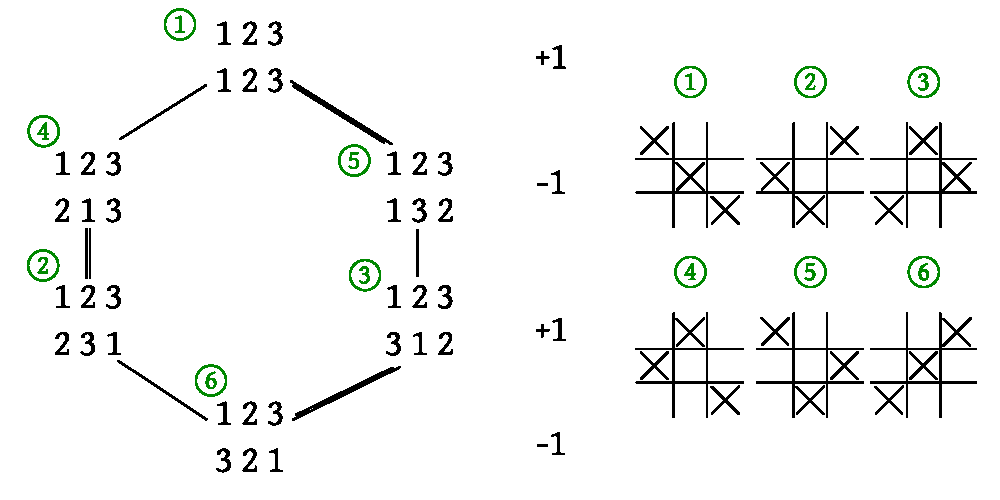
\includegraphics[width=0.45\textwidth]{img/sign-of-permutation.pdf}
      \caption{Sign of a permutation}
      \label{img:perm-sign}
    \end{center}
  \end{figure}
  %Compare with Figure~\ref{img:perm-sign}.
  %\[
  %  \begin{vmatrix} 1 & 2 & 3 \\ 1 & 2 & 3 \end{vmatrix}
  %  = \begin{vmatrix} 1 & 2 & 3 \\ 1 & 3 & 2 \end{vmatrix}
  %  \to \begin{vmatrix} 1 & 2 & 3 \\ 3 & 2 & 1 \end{vmatrix}
  %  = \begin{vmatrix} 1 & 2 & 3 \\ 3 & 2 & 1 \end{vmatrix}
  %\]
  %\[
  %  \begin{vmatrix} 1 & 2 & 3 \\ 1 & 2 & 3 \end{vmatrix}
  %  \to \begin{vmatrix} 1 & 2 & 3 \\ 2 & 1 & 3 \end{vmatrix}
  %  = \begin{vmatrix} 1 & 2 & 3 \\ 2 & 3 & 1 \end{vmatrix}
  %  = \begin{vmatrix} 1 & 2 & 3 \\ 3 & 2 & 1 \end{vmatrix}
  %\]

  \[ = a_{11} a_{22} a_{33} + a_{21} a_{32} a_{13} + a_{31} a_{12} a_{23} - a_{21} a_{12} a_{33} - a_{11} a_{32} a_{23} - a_{31} a_{22} a_{13} \]
  corresponding to (1) + (2) + (3) + (4) + (5) + (6) in Figure~\ref{img:perm-sign}.
\end{rem}

\begin{figure}[!h]
  \begin{center}
    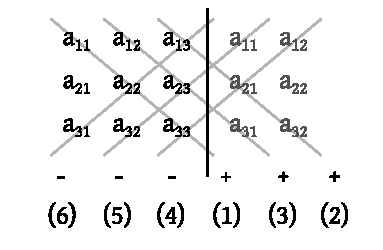
\includegraphics{img/rule_of_sarrus.pdf}
    \caption{Rule of Sarrus visualized}
    \label{img:sarrus}
  \end{center}
\end{figure}

\begin{rem}[Rule of Sarrus]
  Compare with Figure~\ref{img:sarrus}.

  You write the first two columns next to right side of the matrix.
  You add up all 3 diagonals (the product of their values) from top left diagonally to the right bottom
  and subtract all 3 diagonals from left bottom to the top right.

  The rule of Sarrus does not hold for $n=4$!
\end{rem}

\begin{ex}
  \[
    \det\begin{vmatrix} 1 & 2 & 5 \\ 2 & 5 & 14 \\ 5 & 14 & 42 \end{vmatrix}
      = 1 \cdot 5 \cdot 42 + 2 \cdot 14 \cdot 5 + 5 \cdot 2 \cdot 14
      - 5 \cdot 5 \cdot 5 - 14 \cdot 14 \cdot 1 - 2 \cdot 2 \cdot 42
  \] \[
    = 14 (1 \cdot 5 \cdot 3 + 2 \cdot 5 + 5 \cdot 2 - 14 - 2 \cdot 2 \cdot 3) - 125
    %= 14 (15 + 10 + 10 - 14 - 12) - 125
    = 14 \cdot 9 - 125 = 1
  \]

  It turns out, if we use Catalan numbers, we always end up with determinant $1$.
\end{ex}

\begin{lemma}
  Let A be an upper triangular matrix, hence $a_{ij} = 0 \forall i > j$.
  Then it holds that $\det{A} = a_{11} a_{22} \ldots a_{nn}$.
\end{lemma}
\begin{proof}
  \[ \det{A} = \sum_{\pi \in \sigma_n} \sign{\pi} a_{\pi(1),1} \ldots a_{\pi(n),n} \]
  it must hold that
  \[ \pi(j) \leq j \qquad \forall j \]
  \[ \Rightarrow \pi(1) = 1, \pi(2) = 2, \ldots, \pi(n) = n \]
  The only permutation which contributes something is the identity.
  And $\sign{\text{id}} = 1$, hence
  \[ = 1 \cdot a_{11} a_{22} \ldots a_{nn} \]
\end{proof}

\begin{lemma}[Elementary row and column transformations]
  \label{lemma-7.33}
  \[ A = [a_{ij}] \in \mathbb K^{n \times n} \]
  \begin{enumerate}
    \item
      \[ s_i = \begin{bmatrix} a_{1i} \\ \vdots \\ a_{ni }\end{bmatrix} \text{ column vectors} \]
      \[ \Rightarrow \det[as_1, \ldots, s_i + \lambda s_j, \ldots, s_n] = \det(A) \qquad i \neq j \]
    \item
      Let $z_i = [a_{i_1}, \ldots, a_{i_n}] \qquad \text{ rows of $A$}$.
      \[ \det\begin{bmatrix} z_1 \\ \vdots \\ z_i + \lambda z_j \\ \vdots \\ z_n = \end{bmatrix} = \det{A} \qquad \text{ for } i \neq j \]
  \end{enumerate}
\end{lemma}
\begin{proof}
  \begin{enumerate}
    \item compare with determinant form
    \item $\det{A} = \det{A^T}$
  \end{enumerate}
\end{proof}

\begin{ex}
  \label{example-7.34}
  \[
    \begin{vmatrix}
      1 & 2 & 5 \\
      2 & 5 & 14 \\
      5 & 14 & 42
    \end{vmatrix}
    =
    \begin{vmatrix}
      1 & 2 & 5 \\
      0 & 1 & 4 \\
      0 & 4 & 17
    \end{vmatrix}
    =
    \begin{vmatrix}
      1 & 2 & 5 \\
      0 & 1 & 4 \\
      0 & 0 & 1
    \end{vmatrix}
    = 1 \cdot 1 \cdot 1
    = 1
  \]
\end{ex}


\meta{lecture}{14th of March 2016}{Franz Lehner}

\begin{lemma}
  Recall: The following operations do not change the determinant:
  \begin{itemize}
    \item $\triangle(s_1, \ldots, s_i + \lambda s_j, \ldots, s_n) = \triangle(s_1, \ldots, s_n)$ \\
      Addition of a multiple of a column (or row) to another
    \item Gauss-Jordan operations (elementary row/column transformations)
  \end{itemize}
\end{lemma}

\begin{ex}
  \[
    \begin{vmatrix}
      1 & 0 & 3 & -2 \\
      2 & 6 & 4 & 1 \\
      3 & 3 & -1 & -1 \\
      -1 & 2 & 4 & 1
    \end{vmatrix}
    \leadsto
    \begin{vmatrix}
      1 & 0 & 3 & -2 \\
      0 & 6 & -2 & 5 \\
      0 & 3 & -10 & 5 \\
      0 & 2 & 7 & -1
    \end{vmatrix}
    \leadsto
    \frac13
    \frac12
    \begin{vmatrix}
      1 & 0 & 3 & -2 \\
      0 & 6 & -2 & 5 \\
      0 & 6 & -20 & 10 \\
      0 & 6 & 21 & -3
    \end{vmatrix}
  \]
  We multiplied the third row times $2$ and the fourth row times $3$.
  Be aware that this way we avoided fractions in the matrix.

  \[
    \leadsto
    \frac16
    \begin{vmatrix}
      1 & 0 & 3 & -2 \\
      0 & 6 & -2 & 5 \\
      0 & 0 & -18 & 5 \\
      0 & 0 & 23 & -8
    \end{vmatrix}
    \cdot \frac{23}{18}
    = \frac16
    \begin{vmatrix}
      1 & 0 & 3 & -2 \\
      0 & 6 & -2 & 5 \\
      0 & 0 & -8 & 5 \\
      0 & 0 & 0 & -8+5\frac{23}{18}
    \end{vmatrix}
  \]
  Even though we have a fraction $\frac16$ at the front, our result will
  remain to be integral (i.e. without decimal points).

  Triangular matrix:
  \[ \frac16 \cdot 1 \cdot 6 \cdot (-18) \cdot \left(-8 + \frac{5 \cdot 23}{18}\right) \]
  \[ = -(-18\cdot 8 + 5\cdot 23) = -(-144 + 115) = 29 \]
\end{ex}

\begin{lemma}
  \label{lemma-7.35}
  \begin{enumerate}
    \item
      \[
        \begin{array}{|c|ccc|}
          \hline
            a_{11} & * & \ldots & * \\
          \hline
            0      &   &        &  \\
            \vdots &   &  B     &  \\
            0      &   &        &
        \end{array}
        = a_{11} \cdot \det{B}
      \]
    \item
      \[
        \begin{array}{|ccc|c|}
          \hline
                &        &   & 0 \\
                & B      &   & 0  \\
                &        &   & \vdots \\
          \hline
            *   & \ldots & * & a_{nn}
        \end{array}
        = \det{B} \cdot a_{nn}
      \]
  \end{enumerate}
\end{lemma}

\begin{proof}
  \[ \det{A} = \sum_{\pi \in \sigma_n} (-1)^\pi a_{\pi(1),1} \ldots a_{\pi(2),2} \]

  \begin{enumerate}
    \item[2.]
      \begin{align*}
        a_{\pi(n),n} &= 0 \text{ except when } \pi(n) = n \\
          &= \sum_{\pi \in \sigma_n} (-1)^\pi a_{\pi(1),1} \ldots a_{\pi(n),n} \\
          &= \sum_{\rho \in \sigma_{n-1}} (-1)^\rho a_{\rho(1),1} \ldots a_{\rho(n-1),n-1} a_{\rho(n),n}
          &= \det{B} \cdot a_{nn}
      \end{align*}
  \end{enumerate}
\end{proof}

\begin{defi}
  \label{definition-7.36}
  Let $A \in \mathbb K^{n\times n}$.
  \[ 1 \leq k, l \leq n \]
  $A_{k,l}$ (dimension $(n-1) \times (n-1)$) which is generated by $A$ if you cancel out row $k$ and column $l$.

  \[
    \begin{vmatrix}
      a_{1,1} & \ldots & a_{1,l-1} & a_{1,l+1} & \ldots & a_{1,n} \\
      a_{2,1} & \ldots & a_{2,l-1} & a_{2,l+1} & \ldots & a_{2,n} \\
      \vdots & \vdots & \vdots    & \vdots    & \ddots & \vdots \\
      a_{k-1,1} & \ldots & a_{k-1,l-1} & a_{k-1,l+1} & \ldots & a_{k-1,n} \\
      a_{k+1,1} & \ldots & a_{k+1,l-1} & a_{k+1,l+1} & \ldots & a_{k+1,n} \\
      \vdots & \vdots & \vdots    & \vdots    & \ddots & \vdots \\
      a_{n,1} & \ldots & a_{n,l-1} & a_{n,l+1} & \ldots & a_{n,n}
    \end{vmatrix}
  \]
\end{defi}

\index[English]{Generative theorem of Laplace} % TODO: translate
\index[German]{\foreignlanguage{ngerman}{Entwicklungssatz von Laplace}}
\begin{theorem}[Generative theorem of Laplace (dt. Entwicklungssatz von Laplace)]
  \label{thm:laplace-entwicklung}
  Let $A \in K^{n\times n}$, then it holds that
  \[ \det(A) = \sum_{k=1}^n a_{k,l} \cdot (-1)^{k+l} \cdot \det{A_{k,l}} \]
  Generation to $l$-th column.
  \[ \det{A} = \sum_{l=1}^n a_{k,l} \cdot (-1)^{k+l} \cdot \det{A_{k,l}} \]
  Generation to $k$-th row.
\end{theorem}

\begin{proof}
  $l$-th column is
  \[ a_l = \sum_{k=1}^n a_{kl} e_{k} \]

  \begin{align*}
    \det(A) &= \triangle(a_1, \ldots, a_n) \\
      &= \triangle (a_1, \ldots, a_{l-1}, \sum_{k=1}^n a_{kl} e_k, \ldots, a_n) \\
      &= \sum_{k=1}^n a_{kl} \triangle (a_1, \ldots, a_{l-1}, e_k, \ldots a_n) \\
      &= \sum_{k=1}^n a_{kl}
        \begin{vmatrix}
          a_{11} & \ldots & a_{1,l-1} & 0 & a_{1,l+1} & \ldots & a_{1,n} \\
                 &        &           & \vdots &      &        & \\
                 &        &           & 0      &      &        & \\
          \vdots &        &           & 1      &      &        & \vdots \\
                 &        &           & 0      &      &        & \\
                 &        &           & \vdots &      &        & \\
          a_{n1} & \ldots & a_{n,l-1} & 0 & a_{n,l+1} & \ldots & a_{n,n} \\
        \end{vmatrix}
  \end{align*}
  where $1$ is given on the $k$-th row and the $l$-th column which is $e_k$.

  We exchange the $l$-th column with the $(l-1)$-th, then $(l-2)$-th and so on and so forth \dots
  This requires $(l-1)$ transpositions.

  \[
    \sum_{k=1}^n a_{kl} (-1)^{l-1}
    \begin{vmatrix}
      0 & a_{11} & \ldots & a_{1,l-1} & a_{1,l-1} & \ldots & a_{1,n} \\
      \vdots & a_{21} & \ldots & \ldots & \ldots & \ldots & \ldots \\
      0 & \ldots & \ldots & \ldots & \ldots & \ldots & \ldots \\
      1 & \ldots & \ldots & \ldots & \ldots & \ldots & \ldots \\
      0 & \ldots & \ldots & \ldots & \ldots & \ldots & \ldots \\
      \vdots & \ldots & \ldots & \ldots & \ldots & \ldots & \ldots \\
      0 & a_{n1} & \ldots & a_{n,l-1} & a_{n,l-1} & \ldots & a_{n,n}
    \end{vmatrix}
  \]
  where $1$ is given on the $k$-th row.

  Exchange $k$-th and $(k-1)$-th row, then $(k-2)$-th and so on and so forth \dots
  This requires $k-1$ transpositions.

  \[
    = \sum_{k=1}^n a_{kl} (-1)^{k-1+l-1}
    \begin{array}{|c|c|}
    \hline
      1 & \\
    \hline
      0 & \\
      \vdots & \\
      \ldots & A_{k,l} \\
      \vdots & \\
      0 & \\
    \hline
    \end{array}
    = \sum_{l=1}^n a_{k,l} (-1)^{k+l} \det{A_{k,l}}
  \]
\end{proof}

\begin{ex}
  \[
    \begin{vmatrix}
      1 & 2 & 5 \\
      2 & 5 & 14 \\
      5 & 14 & 42
    \end{vmatrix}
    =
    1 \cdot \begin{vmatrix}
      5 & 14 \\
      14 & 42
    \end{vmatrix} - 2 \cdot \begin{vmatrix}
      2 & 14 \\
      5 & 42
    \end{vmatrix} + 5 \cdot \begin{vmatrix}
      2 & 5 \\
      5 & 4
    \end{vmatrix}
  \] \[
    \begin{array}{|c|c|c|}
      + & - & + \\
    \hline
      - & + & - \\
    \hline
      + & - & +
    \end{array}
  \]
  where the top right $+$ refers to the third summand (submatrix)
  and the top middle $-$ refers to the second summand (submatrix).
  \[
    = (5 \cdot 42 - 14\cdot 14) - 2 \cdot (2 \cdot 42 - 5 \cdot 14) + 5 \cdot (2 \cdot 14 - 5 \cdot 5)
    = 14 - 2 \cdot 14 + 5 \cdot 3 = 1
  \]
\end{ex}

\index[English]{Complementary matrix}
\index[German]{\foreignlanguage{ngerman}{Komplementärmatrix}}
\index[English]{Adjoint matrix}
\index[German]{\foreignlanguage{ngerman}{Adjunkte Matrix}}
\begin{theorem}
  \label{satz-7.39}
  $A$ is invertible iff $\det{A} \neq 0$.

  Let $A \in K^{n \times n}$, $\hat{A} \coloneqq [\hat{a}_{kl}]_{k,l=1,\ldots,n}$
  is the \emph{complementary matrix} or \emph{adjoint matrix}.

  \[ \hat{a}_{kl} = (-1)^{k+l} \det{A_{lk}} \]
  Then
  \[ A^{-1} = \frac{1}{\det{A}} \cdot \hat{A} \]
\end{theorem}
\begin{proof}
  Show that $B \coloneqq \hat{A} \cdot A = \det{A} \cdot I$.
  \[ b_{k,l} = \sum_{j=1}^n \hat{a}_{kj} a_{jl} = \sum_{j=1}^n (-1)^{k+j} \det{A}_{jk} a_{jl} \]
  \begin{description}
    \item[Case $k=l$]
      \[ b_{kk} = \sum_{j=1}^n (-1)^{k+j} a_{jk} \det{A}_{jk} = \det{A} \left(\text{Laplace generation to $k$-th column}\right) \]
    \item[Case $k\neq l$]
      Without loss of generality $k < l$.
      \[
        0 = \det\begin{bmatrix}
          a_{11} & \ldots & a_{1l} & \ldots & a_{1l} & \ldots & a_{1n} \\
          \vdots & \vdots & \vdots & \vdots & \vdots & \vdots & \vdots \\
          a_{n1} & \ldots & a_{nl} & \ldots & a_{nl} & \ldots & a_{nn} \\
        \end{bmatrix}
      \]
      We replace the $k$-th column (left column with $a_{1l}$ in the middle)
      by the $l$-th column (right column with $a_{1l}$ in the middle).

      Laplace generation by $k$-th column:
      \[
        = \sum_{j=1}^n a_{jl} \det\begin{bmatrix}
          a_{11} & \ldots & 0 & \ldots & a_{1l} & \ldots & a_{1n} \\
          \vdots & \vdots & \vdots & \vdots & \vdots & \vdots & \vdots \\
          \vdots & \vdots & 1 & \vdots & \vdots & \vdots & \vdots \\
          \vdots & \vdots & \vdots & \vdots & \vdots & \vdots & \vdots \\
          a_{n1} & \ldots & 0 & \ldots & a_{nl} & \ldots & a_{nn} \\
        \end{bmatrix}
      \]
      Similar to Laplace:
      \[ = \sum_{j=1}^n a_{jl} (-1)^{j+l} \det{A_{jk}} = \sum_{j=1}^n a_{jl} \hat{a}_{kj} = b_{kl} \]
  \end{description}
\end{proof}

\begin{ex}[Cayley 1855]
  Cayley considered it as partial derivations:
  \[
    \frac{1}{\triangledown}
    \begin{vmatrix}
      \partial_a \triangledown & \partial_c \triangledown \\
      \partial_b \triangledown & \partial_d \triangledown \\
    \end{vmatrix}
  \]

  Consider $n=2$:
  \[
    \begin{bmatrix}
      a & b \\
      c & d
    \end{bmatrix}^{-1}
    = \frac{1}{ad - bc}
    \begin{bmatrix}
      d & -b \\
      -c & a
    \end{bmatrix}
  \]

  Consider $n=3$:
  \[
    \begin{bmatrix}
      a_{11} & a_{12} & a_{13} \\
      a_{21} & a_{22} & a_{23} \\
      a_{31} & a_{32} & a_{33}
    \end{bmatrix}^{-1}
    = \frac{1}{\det{A}}
    \begin{bmatrix}
      \begin{vmatrix}
        a_{22} & a_{13} \\
        a_{32} & a_{33}
      \end{vmatrix} &
      - \begin{vmatrix}
        a_{12} & a_{13} \\
        a_{32} & a_{33}
      \end{vmatrix} &
      \begin{vmatrix}
        a_{12} & a_{13} \\
        a_{22} & a_{23}
      \end{vmatrix} \\
      - \begin{vmatrix}
        a_{21} & a_{23} \\
        a_{31} & a_{33}
      \end{vmatrix} &
      \begin{vmatrix}
        a_{11} & a_{13} \\
        a_{31} & a_{33}
      \end{vmatrix} &
      -\begin{vmatrix}
        a_{11} & a_{13} \\
        a_{21} & a_{23}
      \end{vmatrix} \\
      \begin{vmatrix}
        a_{21} & a_{22} \\
        a_{31} & a_{32}
      \end{vmatrix} &
      - \begin{vmatrix}
        a_{11} & a_{12} \\
        a_{31} & a_{32}
      \end{vmatrix} &
      \begin{vmatrix}
        a_{11} & a_{12} \\
        a_{21} & a_{22}
      \end{vmatrix}
    \end{bmatrix}
  \]
\end{ex}

\begin{ex}
  \[
    \begin{bmatrix}
      1 & 2 & 5 \\
      2 & 5 & 14 \\
      5 & 14 & 42
    \end{bmatrix}
    =
    \begin{bmatrix}
      \begin{vmatrix}
        5 & 14 \\
        14 & 42
      \end{vmatrix} &
      - \begin{vmatrix}
        2 & 5 \\
        14 & 42 \\
      \end{vmatrix} &
      \begin{vmatrix}
        2 & 5 \\
        5 & 14
      \end{vmatrix} \\
      -\begin{vmatrix}
        2 & 14 \\
        5 & 42
      \end{vmatrix} &
      \begin{vmatrix}
        1 & 5 \\
        5 & 42
      \end{vmatrix} &
      -\begin{vmatrix}
        1 & 5 \\
        2 & 14
      \end{vmatrix} \\
      \begin{vmatrix}
        2 & 5 \\
        5 & 14
      \end{vmatrix} &
      -\begin{vmatrix}
        1 & 2 \\
        5 & 14
      \end{vmatrix} &
      \begin{vmatrix}
        1 & 2 \\
        2 & 5
      \end{vmatrix}
    \end{bmatrix}
    = \begin{bmatrix}
      14 & -14 & 3 \\
      -14 & 17 & -4 \\
      3 & -4 & 1
    \end{bmatrix}
  \] \[
    \begin{vmatrix}
      5 & 14 \\
      14 & 42
    \end{vmatrix}
    = 5 \cdot 3 \cdot 14
    - 14 \cdot 14 = 14
  \] \[
    \begin{vmatrix}
      2 & 5 \\
      14 & 42
    \end{vmatrix}
    = 2 \cdot 3 \cdot 14
    - 5 \cdot 14 = 14
  \]
\end{ex}

\begin{theorem}[Arnold's hypothesis]
  \enquote{No theorem in mathematics is named after it's original author}
\end{theorem}
\begin{proof}
  No proof provided here.
\end{proof}

\begin{theorem}[Cramer's rule]
  Originally by McLansin (1748) based on work by Leibniz (1678) and reformulated by G. Cramer (1750).

  A regular $n\times n$ matrix with column vectors $a_1, \ldots, a_n \in \mathbb K^n$.

  Then the unique solution to the equation system $Ax = b$ is given by
  \[
    x_i \coloneqq
    \frac{\triangle(a_1, \ldots, a_{i-1}, b, a_{i+1}, \ldots, a_n)}{\triangle(a_1, \ldots, a_n)}
    = \frac{\det(a_1,\ldots,b,\ldots,a_n)}{\det{A}}
  \]

  Its complexity is given by $n+1$ determinants!
\end{theorem}
\begin{proof}
  \[ b = \sum_{j=1}^{n} b_j e_j \]
  \[ x = A^{-1} b - \frac{1}{\det{A}} \hat{A} \cdot b \]
  \[ x_i = \frac{1}{\det{A}} \sum_{j=1}^{n} \hat{a}_{ij} b_j = \frac{1}{\det{A}} \sum_{j=1}^{n} (-1)^{i+j} \det{(A_j)} b_j \]
  \[ = \frac{1}{\det{A}} \sum_{j=1}^n \triangle (a_1, \ldots, a_{i-1}, \ldots, a_{j-1}, e_j, a_{j+1}, \ldots, a_n) \cdot b_j \]
  \[ = \frac{1}{\det{A}} \triangle (a_1, \ldots, a_{i-1}, \underbrace{\sum_{j=1}^n b_j e_j}_{=b}, \ldots, a_n) \]
\end{proof}

% TODO: in the following indices are missing

\begin{ex}
  \label{exercise-7.42}
  \[ 2x_1 + 2x_2 = 7 \]
  \[ x_1 - 3x_2 = 0 \]
  \[ A = \begin{bmatrix} 2 & 2 \\ 1 & -3 \end{bmatrix} \qquad b = \begin{bmatrix} 7 \\ 0 \end{bmatrix} \]
  \[
    \det{A} = -8 \qquad
    x_1 = \frac{\begin{vmatrix} 7 & 2 \\ 0 & -3 \end{vmatrix}}{-8} = \frac{21}{8} \qquad
    x_2 = \frac{\begin{vmatrix} 2 & 7 \\ 1 & 0 \end{vmatrix}}{-8} = \frac78
  \]
\end{ex}
\begin{rem}
  \label{bem-7.43}
  \begin{itemize}
    \item in higher dimensions ($n \geq 4$)
      Cramer's rule is disallowed.
      \begin{enumerate}
        \item too computationally intense
        \item numerically unstable (small errors have large effects)
      \end{enumerate}
    \item Anyways, still useful for theoretical considerations
      \begin{enumerate}
        \item the map $A \mapsto \det{A}$ is $C^\infty$ (polynomial!) (this denotes infinite differentiability)
        \item The set of invertible matrices in $\mathbb R^{n\times n}$ is open,
          because if $\det{A} \neq 0$, then also $\det{\tilde{A}} \neq 0$ as long as $\abs{a_{ij} - \tilde{a}_{ij}} < \delta$.
        \item The solution of the equation system $Ax = b$, for invertible $A$, depends continuously and differentiable
          on $A$ and $b$:
          \[
            x_i
            = \underbrace{\frac{1}{\det{A}}}_{\text{continuous as long as } \det{A} \neq 0} \underbrace{\hat{A} b}_{\text{polynomial}}
          \]
        \item The map $\operatorname{GL}(n,\mathbb R) \to \operatorname{GL}(n,\mathbb R)$
          \[ A \mapsto A^{-1} \]
          is continuous.
          \[ A^{-1} = \frac{1}{\det{A}} \cdot \hat{A} \]
          So $\operatorname{GL}(n,\mathbb R)$ is a Lie group.
      \end{enumerate}
  \end{itemize}
\end{rem}

\meta{lecture}{16th of March 2016}{Franz Lehner}

\section{Inner products}
%
Descartes introduced \enquote{La G\'eometrie} (1637).

\begin{defi}
  The length of a vector in $\mathbb R^2/\mathbb R^3$ is:
  \[ \left\| \begin{pmatrix} x_1 \\ x_2 \\ x_3 \end{pmatrix} \right\| = \sqrt{x_1^2 + x_2^2 + x_3^2} \]
\end{defi}

\begin{figure}[!h]
  \begin{center}
    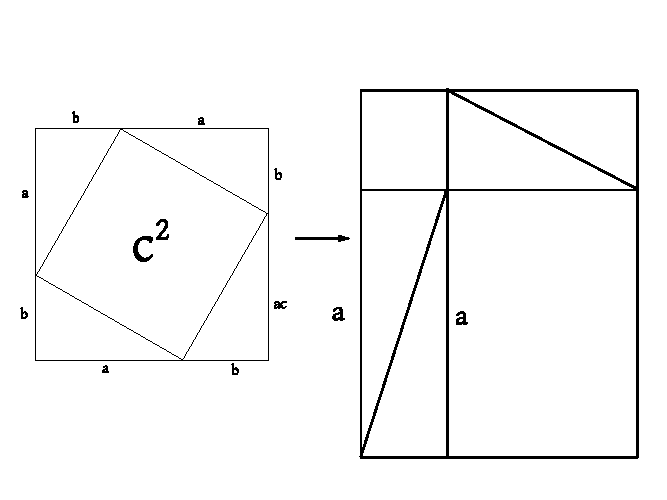
\includegraphics{img/pythagorian-proof.pdf}
    \caption{Pythagorian proof of $c^2 = a^2 + b^2$}
    \label{img:pyth}
    % TODO
  \end{center}
\end{figure}

\begin{defi}[Scalar product]
  \[ \cos{\theta} = \cos(2\pi - \theta) \]
  The scalar product is defined as
  \[ \functional{a,b} = \norm{a} \cdot \norm{b} \cdot \cos{\theta} \]
\end{defi}

\begin{theorem}
  \label{prop-8.2}
  The following properties hold:
  \begin{itemize}
    \item $\norm{\lambda \cdot a} = \abs{\lambda} \cdot \norm a$
    \item $\norm{a + b} \leq \norm{a} + \norm{b}$ (triangle inequality)
    \item $\functional{a,a} = \norm{a}^2 \geq 0$
    \item $\functional{a,a} = 0 \Leftrightarrow a = 0$
    \item $\functional{a,b} = 0 \Leftrightarrow a = 0 \lor b = 0$
      \[ \functional{a,b} > 0 \Leftrightarrow \text{ acute angle } \]
      \[ \functional{a,b} < 0 \Leftrightarrow \text{ obtuse angle } \]
  \end{itemize}
\end{theorem}

\begin{theorem}
  \label{satz-8.3}
  \begin{align}
    \functional{a,b} &= \functional{b,a} \\
    \functional{\lambda a,b} &= \lambda \functional{a,b} \\
    \functional{a+b,c} &= \functional{a,c} + \functional{b,c}
  \end{align}
  So it actually describes a bilinear map.
\end{theorem}

\begin{proof}
  \begin{itemize}
    \item immediate
    \item
      \begin{description}
        \item[$\lambda > 0$]
          immediate
        \item[$\lambda < 0$]
          Angle $\theta$ becomes $\pi - \theta$.
          \[ \cos(\pi - \theta) = -\cos{\theta} \]
          \[ \functional{\lambda a,b} = \abs{\lambda} \cdot \norm{a} \cdot \norm{b} \cos(\pi - \theta) = -\abs{\lambda} \cdot \norm{a} \cdot \norm{b} \cdot \cos{\theta} = \lambda \functional{a,b} \]
      \end{description}
    \item
      Let $b = e, \norm{e} = 1$.
      \[ \functional{a,e} = \norm{a} \cdot \cos{\theta} \]
      \[ \functional{a+b,c} = \norm{c} \functional{a+b,\frac{c}{\norm{c}}} - \norm{c} \left(\functional{a,\frac{c}{\norm{c}}} + \functional{b,\frac{c}{\norm{c}}}\right) = \functional{a,c} + \functional{b,c} \]
      Compare with Figure~\ref{img:383}.
      \begin{figure}[!h]
        \begin{center}
          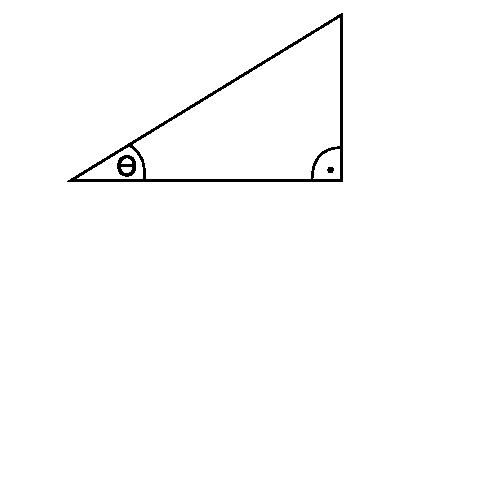
\includegraphics{img/8_3_3.pdf}
          \caption{$\functional{a+b,c} = \functional{a,c} + \functional{b,c}$}
          \label{img:383}
        \end{center}
      \end{figure}
  \end{itemize}
\end{proof}

\begin{theorem}
  \label{satz-8.4}
  \[ \functional{\begin{pmatrix} a_1 \\ a_2 \\ a_3 \end{pmatrix}, \begin{pmatrix} b_1 \\ b_2 \\ b_3 \end{pmatrix}} = a_1 b_1 + a_2 b_2 + a_3 b_3 \]
\end{theorem}
\begin{proof}
  \begin{align*}
    \functional{a,b} &= \functional{a_1 e_1 + a_2 e_2 + a_3 e_3, b} \\
      &= a_1 \functional{e_1, b} + a_2 \functional{e_2, b} + a_3 \functional{e_3, b} \\
      &= a_1 b_1 + a_2 b_2 + a_3 b_3 \\
    \functional{e_i,b}
      &= \functional{e_i, b_1 e_1 + b_2 e_2 + b_3 e_3} \\
      &= b_1 \functional{e_i, e_1} + b_2 \functional{e_i, e_2} + b_3 \functional{e_i, e_3} \\
      &= b_1 \delta_{i1} + b_2 \delta_{i2} + b_3 \delta_{i3} \\
      &= b_i
  \end{align*}
  with $\dim\functional{e_i,e_j} = \delta_{ij}$.
\end{proof}

\begin{ex}[Law of cosines]
  \label{ex-8.5}
  \[ a^2 + b^2 = c^2 + 2ab \cos{\gamma} \]
  Compare with Figure~\ref{img:law-of-cosines}.
  \begin{figure}[!h]
    \begin{center}
      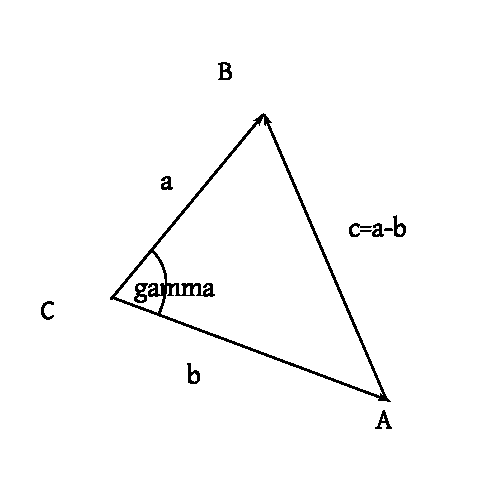
\includegraphics{img/law-of-cosines.pdf}
      \caption{Law of cosines}
      \label{img:law-of-cosines}
    \end{center}
  \end{figure}

  \begin{align*}
    \norm{c}^2 &= \functional{a-b, a-b} \\
      &= \functional{a,a} - \functional{a,b} - \functional{b,a} + \functional{b,b} \\
      &= \norm{a}^2 - 2 \cdot \norm{a} \norm{b} \cos{\gamma} + \norm{b}^2
  \end{align*}
\end{ex}

\begin{theorem}{Theorem by Thales}
  TODO: image
  \begin{align*}
    \functional{a-b, -a-b} &= \norm{a-b} \norm{a+b} \cos\theta \\
    \functional{a-b, -a-b} &= -\functional{a-b, a+b} \\
      &= -\left(\functional{a,a} - \functional{b,a} + \functional{a,b} - \functional{b,b}\right) \\
      &= -\left(\norm{a}^2 - \norm{b}^2\right) \\
      &= 0 \\
      &\Rightarrow \theta = \frac\pi2
  \end{align*}
\end{theorem}

\begin{rem}
  How do we find the normal vector?
  \[ \vec{n} = \begin{pmatrix} a_2 \\ -a_1 \end{pmatrix} \]
  \[ \functional{\begin{pmatrix} a_1 \\ a_2 \end{pmatrix}, \begin{pmatrix} a_2 & -a_1 \end{pmatrix}} = a_1 a_2 - a_2 a_1 = 0 \]
\end{rem}

\begin{defi}[Outer product]
  \enquote{Outer product}, \enquote{cross product} or \enquote{vector product}

  TODO: image missing

  This is only available in $\mathbb R^3$.

  Let $a,b \in \mathbb R^3$, then $a \times b$ is the vector with properties:
  \begin{itemize}
    \item $\norm{a \times b} = \norm{a} \cdot \norm{b} \cdot \sin\theta$ \\
      This corresponds to the are of a parallelogram.
      \[ \norm{b} \cdot \sin\theta = \text{ heigh of a parallelogram} \]
    \item $a \times b \bot a,b$
      \begin{align*}
        \functional{a \times b, a} &= 0 \\
        \functional{a \times b, b} &= 0
      \end{align*}
    \item $(a,b,a\times b)$ are clockwise (consider a screw coming out of Figure)
      \[ a \times b = 0 \Leftrightarrow a = 0 \lor b = 0 \lor a,b \text{ are linear dependent} \]
  \end{itemize}
\end{defi}

\begin{theorem}
  \label{satz-8.8}
  \begin{enumerate}
    \item $b \times a = - a \times b$ (counter-clockwise)
    \item $(\lambda a) \times b = \lambda \cdot a \times b = a \times (\lambda b)$
    \item $(a + b) \times c = a \times c + b \times c$
  \end{enumerate}
  So it is bilinear in $\mathbb R^3 \times \mathbb R^3 \to \mathbb R^3$
\end{theorem}

\begin{proof}
  \[ a \times c, b \times c, (a + b) \times c \in E \]
  Let $a',b',(a+b)'$ be the projection of $a, b$ and $a+b$ in the plane.
  \begin{figure}
    \begin{center}
      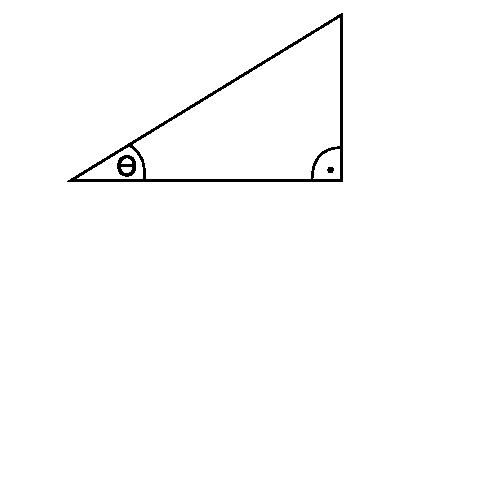
\includegraphics{img/8_3_3.pdf} % TODO
      \caption{Theorem~\ref{satz-8.8}, third statement}
    \end{center}
  \end{figure}

  TODO: image missing
  \begin{enumerate}
    \item
      \[ (a + b)' = a' + b' \]
      Projection of the sum = sum of projections.
    \item
      \[ a \times c = a' \times c \]
      \[ \norm{a' \times c} = \norm{a'} \cdot \norm{c} \]
      \begin{align*}
          \norm{a \times c} &= \norm{a} \cdot \norm{c} \cdot \sin{\theta} \\
            &= \norm{a'} \cdot \norm{c}
      \end{align*}
      \[ \norm{a'} = \norm{c} \cdot \sin\theta \]
      and they have the same direction.

      TODO: image missing
    \item
      \[ (a' + b') \times c = c' \times c + b' \times c \]
      From above:

      TODO: image missing

      \[ \norm{a' \times c} = \norm{c} \cdot \norm{a'} \]
  \end{enumerate}
  So this operation is linear.

  \begin{align*}
    (a + b) \times c
      &\stackrel{2}{=} (a + b)' \times c \\
      &\stackrel{1}{=} (a' + b') \times c \\
      &\stackrel{3}{=} (a' \times c + b' \times c) \\
      &\stackrel{2}{=} a \times c + b \times c
  \end{align*}
\end{proof}

\begin{cor}
  \label{cor-8.9}
  The cross product is a map $x: \mathbb R^3 \to \mathbb R^3 \to \mathbb R^3$
  with properties:
  \begin{itemize}
    \item bilinear
    \item anti-symmetric
    \item \enquote{chiral}, namely
      \[ e_1 \times e_2 = e_3 \]
      \[ e_2 \times e_3 = e_1 \]
      \[ e_3 \times e_1 = e_2 \]
  \end{itemize}
\end{cor}

\begin{cor}
  \label{cor-8.10}
  \[
    \begin{pmatrix}
      a_1 \\ a_2 \\ a_3
    \end{pmatrix} \times
    \begin{pmatrix}
      b_1 \\ b_2 \\ b_3
    \end{pmatrix}
    = \begin{bmatrix}
      a_2 b_3 - a_3 b_2 \\
      a_3 b_1 - a_1 b_3 \\
      a_1 b_2 - a_2 b_1
    \end{bmatrix}
    = \begin{bmatrix}
      \begin{vmatrix}
        a_2 & b_2 \\
        a_3 & b_3
      \end{vmatrix} \\
      -
      \begin{vmatrix}
        a_1 & b_1 \\
        a_3 & b_3
      \end{vmatrix} \\
      \begin{vmatrix}
        a_2 & b_2 \\
        a_2 & b_2
      \end{vmatrix}
    \end{bmatrix}
  \] \[
    \overset{\text{Laplace}}{=}
    \begin{vmatrix}
      a_1 & b_1 & e_1 \\
      a_2 & b_2 & e_2 \\
      a_3 & b_3 & e_3
    \end{vmatrix}
  \]
  Formally, matrices in a vector of values are disallowed,
  but as far as it boils down to addition, this is fine.
\end{cor}

\begin{proof}
  \begin{align*}
    & (a_1 e_1 + a_2 e_2 + a_3 e_3) \times (b_1 e_1 + b_2 e_2 + b_3 e_3) \\
    &= a_1 b_1 e_1 \times e_1 + a_1 b_2 e_1 \times e_2 + a_1 b_3 e_1 \times e_3 \\
    &+ a_2 b_1 e_2 \times e_1 + a_2 b_2 e_2 \times e_2 + a_2 b_3 e_3 \times e_3 \\
    &+ a_3 b_1 e_3 \times e_1 + a_3 b_2 e_3 \times e_2 + a_3 b_3 e_3 \times e_3 \\
    &= a_1 b_2 e_3 + a_1 b_3 (-e_2)
    + a_2 b_1 (-e_3) + a_2 b_3 e_1 +
    a_3 b_1 e_2 + a_3 b_2 (-e_1) \\
    &= (a_2 b_3 - a_3 b_2) e_1 + (a_3 b_1 - a_1 b_3) e_2 + (a_1 b_2 - a_2 b_1) e_3
  \end{align*}
\end{proof}

\begin{theorem}[Scalar triple product]
  \label{satz-8.11}
  The three-dimensional parallelogram is called \enquote{Spat} in German (compare with Figure~\ref{img:3dp}).
  \[
    \functional{a\times b, c}
    = \begin{vmatrix}
      a_1 & b_1 & c_1 \\
      a_2 & b_2 & c_2 \\
      a_3 & b_3 & c_3
    \end{vmatrix}
    = \text{ volume of spanned 3-dimensional parallelogram}
  \]
  \begin{figure}[!h]
    \begin{center}
      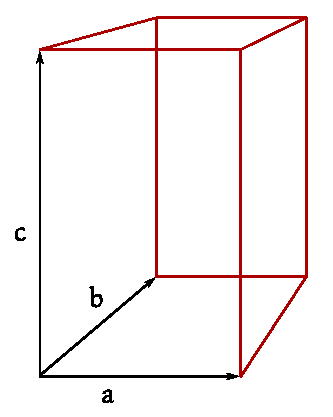
\includegraphics{img/scalar-triple-product.pdf}
      \caption{Three-dimensional parallelogram}
      \label{img:3dp}
    \end{center}
  \end{figure}
  $\norm{a \times b}$ is the area of the parallelogram.
  $\functional{a \times b, c} = \norm{a \times b} \cdot \norm{c} \cdot \cos\theta$
  where $\norm{c} \cdot \cos\theta$ is the height of the $3$-dimensional parallelogram.

  \[
    \functional{a \times b, c} = \functional{
      \begin{pmatrix}
        \begin{vmatrix}
          a_1 & b_2 \\
          a_3 & b_3
        \end{vmatrix} \\
        - \begin{vmatrix}
          a_1 & b_1 \\
          a_3 & b_3
        \end{vmatrix} \\
        \begin{vmatrix}
          a_1 & b_1 \\
          a_2 & b_2
        \end{vmatrix}
      \end{pmatrix},
      \begin{pmatrix} c_1 \\ c_2 \\ c_3 \end{pmatrix}
    }
  \] \[
    \begin{vmatrix} a_2 & b_2 \\ a_3 & b_3 \end{vmatrix} \cdot c_1
    - \begin{vmatrix} a_1 & b_1 \\ a_3 & b_3 \end{vmatrix} \cdot c_2
    + \begin{vmatrix} a_1 & b_1 \\ a_2 & b_2 \end{vmatrix} \cdot c_3
    = \text{Laplace generated by third column}
  \]
\end{theorem}
\begin{ex}
  \label{application-8.12}
  Given a plane in parameter representation:
  \[ E = \setdef{v_0 + \lambda a + \mu b}{\lambda, \mu \in \mathbb R} \]
  Find $\alpha_1, \alpha_2, \alpha_3$ and $\beta$ with (\enquote{implicit representation})
  \[ E = \setdef{x}{\alpha_1 x_1 + \alpha_2 x_2 + \alpha_3 x_3 = \beta}\]
  \[
    \begin{pmatrix} \alpha_1 \\ \alpha_2 \\ \alpha_3 \end{pmatrix}
    = a \times b
  \]
  TODO: image missing
  \[ \beta = \functional{v_0, a \times b} \]
\end{ex}

In the following chapters we always consider $\mathbb K = \mathbb R$ or $\mathbb K = \mathbb C$.

\index[English]{Inner product}
\index[German]{\foreignlanguage{ngerman}{Inneres Produkt}}
\index[English]{Semi-definite inner product}
\index[German]{\foreignlanguage{ngerman}{Semi-definites inneres Produkt}}
\index[English]{Definite inner product}
\index[German]{\foreignlanguage{ngerman}{Definites inneres Produkt}}
\index[English]{Positive Semi-definite inner product}
\index[German]{\foreignlanguage{ngerman}{Positives semi-definites inneres Produkt}}
\index[English]{Positive definite inner product}
\index[German]{\foreignlanguage{ngerman}{Positives definites inneres Produkt}}
\index[English]{Negative Semi-definite inner product}
\index[German]{\foreignlanguage{ngerman}{Negatives semi-definites inneres Produkt}}
\index[English]{Negative definite inner product}
\index[German]{\foreignlanguage{ngerman}{Negatives definites inneres Produkt}}
\index[English]{Indefinite inner product}
\index[German]{\foreignlanguage{ngerman}{Indefinites inneres Produkt}}
\begin{defi}
  \label{defi-8.13}
  An inner product over a vector space in $\mathbb R$ or $\mathbb C$
  is a map $\functional{\cdot, \cdot}: V \times V \to \mathbb K$
  with properties:
  \begin{itemize}
    \item $\functional{x+y, z} = \functional{x,z} + \functional{y,z} \quad \forall x,y,z \in V$
    \item $\functional{\lambda x, y} = \lambda \functional{x,y} \quad \forall x,y \in V \forall \lambda \in \mathbb K$
    \item $\functional{y,x} = \overline{\functional{x,y}} \quad \forall x,y \in V$
  \end{itemize}
  where $\overline{\functional{x,y}}$ denotes the complex conjugate.
  Especially $\functional{x,x} \in \mathbb R \forall x \in V$.

  An inner product is called
  \begin{description}
    \item[positive semidefinite] if $\functional{x,x} \geq 0 \quad \forall x$
    \item[positive definite] if $\functional{x,x} > 0 \quad \forall x \neq 0$
    \item[negative semidefinite] if $\functional{x,x} \leq 0 \quad \forall x$
    \item[negative definite] if $\functional{x,x} < 0 \quad \forall x \neq 0$
    \item[indefinite] if $\exists x: \functional{x,x} > 0 \land \exists y: \functional{y,y} < 0$
  \end{description}
\end{defi}

% TODO: check translations
\begin{defi}
  Scalar product if $\mathbb K = \mathbb R$ \\
  Hermitian product (or unitary product) if $\mathbb K = \mathbb C$ \\

  Quadratic form if $\mathbb K = \mathbb R$ \\
  Hermitian form if $\mathbb K = \mathbb C$
\end{defi}

\begin{lemma}
  \begin{itemize}
    \item $\functional{x,y+z} = \functional{x,y} + \functional{x,z}$
    \item $\functional{x,\lambda y} = \overline{\lambda} \functional{x,y}$
    \item $\functional{x,0} = 0$
  \end{itemize}
  Linear in $x$ and anti-linear in $y$!

  Sesquilinear.
\end{lemma}


\meta{lecture}{11th of April 2016}{Franz Lehner}

% (a)
Scalar product.
\begin{enumerate}
  \item Not bilinear, but sequilinear
    \begin{itemize}
      \item $\functional{x+y, z} = \functional{x,z} + \functional{y,z}$
      \item $\functional{\lambda x, y} = \lambda \functional{x,y}$
      \item $\functional{x,y} = \overline{\functional{y,x}}$ (hermetian)
    \end{itemize}
  \item $\functional{,}$ is called positive definite, if
    \[ \functional{x,x} > 0 \qquad \forall x \neq 0 \]
    \begin{tabular}{cl}
      $\geq 0$ & positive semidefinite \\
      $<0$ & negative definite \\
      $\leq$ & negative semidefinite \\
      $\neq$ & indefinite
    \end{tabular}
\end{enumerate}

\subsection{Examples}
\label{ex-8.15}

\begin{itemize}
  \item $\mathbb R^n$:
    \[
      \left\langle\begin{bmatrix} x_1 \\ \vdots \\ x_n \end{bmatrix}\right\rangle,
       \left\langle\begin{bmatrix} y_1 \\ \vdots \\ y_n \end{bmatrix}\right\rangle
       = \sum_{x=1}^n x_i y_i = x^t y
    \]
  \item $\mathbb C^n$
    \[ \functional{x,y} = \sum_{i=1}^n x_i \overline{y_i} = x^t \overline{y} \]
  \item
    $A = [a_j]_{j=1,\ldots,n}$ because $\functional{x,y}_A = x^t A y$ is complex.
\end{itemize}

Exercise: is symmetrical if and only if $A = A^t$, hence $a_{ij} = a_{ji}$. \\
Exercise: is hermetian if and only if $a_{ij} = \overline{a_{ji}}$ ($A$ is hermitian)


$\dim = \infty$.
\[ \mathbb R^\infty: \functional{x,y} = \sum_{i=1}^\infty x_n y_n \]
% TODO: "... der Reihe konvergent"
Development on $l^2 = \setdef{(x_i)}{\sum_{\abs{x_i}^2} < \infty}$
where $l$ stands for Lebeque.

$\Rightarrow$ Hilbert space.

% (e)
\[ V = C([a,b], \mathbb C) \]
\[ \functional{f,g} = \int_a^b f(x) \overline{g(x)} \, dx \]

\subsection{Norm}
%
\index[English]{Norm}
\index[German]{\foreignlanguage{ngerman}{Norm}}
\begin{defi}
  \label{def-8.16}
  A \emph{norm} on a vector space $V$ over $\mathbb R$ or $\mathbb C$ is a mapping
  $\| \, \| \to [0,\infty[$ with properties
  \begin{itemize}
    \item[N1.] $\norm{X} \geq 0 \, \forall X$, $\norm{X} = 0 \Leftrightarrow X = 0$
    \item[N2.] $\norm{\lambda X} = \norm{\lambda} \cdot \norm{X}$ (homogeneous)
    \item[N3.] $\norm{X + Y} \leq \norm{X} + \norm{Y}$ (triangle inequality)
  \end{itemize}
\end{defi}

\begin{rem}
  \label{rem-8.17}
  A norm induces a metric.
  \[ d(x,y) = \norm{x - y} \]
  The induced metric satisfies
  \[ d(x+z, y+z) = d(x,y) \]
\end{rem}

\index[English]{Euclidean norm}
\index[German]{\foreignlanguage{ngerman}{Euklidische Norm}}
\begin{ex}
  \label{example-8.18}
  \begin{itemize}
    \item
      In $\mathbb R^n/\mathbb C^n$
      \[ \norm{X}_{\infty} = \max(\norm{X_1}, \ldots, \norm{X_n}) \]
      The \emph{euclidean norm} is given by:
      \[ \norm{X}_2 = \left(\sum \norm{X}^2\right)^{\frac 12} \]
      The $L^1$-norm is given by (compare it with possible paths in a grid)
      \[ \norm{X}_1 = \sum_{i=1}^n \norm{X_i} \]
    \item
      Analogously for $V = C[a,b]$
        \[ \norm{f}_{\infty} = \sup_{x \in [a,b]} \norm{f(x)} \]
        \[ \norm{f}_2 = \left(\int_a^b \norm{f(x)}^2 \, dx\right)^{\frac 12} \]
        \[ \norm{f}_1 = \int_a^b \norm{f(x)} \, dx \]
  \end{itemize}
\end{ex}

\begin{theorem}
  \label{satz-8.19}
  Let $\functional{,}$ be a positive definite scalar product in $V$.
  Then $\norm{X} = \sqrt{\functional{x,x}}$ defines a norm in $V$.
\end{theorem}
\begin{proof}
  \begin{enumerate}
    \item[N1.]
      \[ \functional{x,x} \geq 0 \Rightarrow \sqrt{\,} \text{ is  well-defined in } \mathbb R^+ \]
      \[ \norm{X} = 0 \Leftrightarrow \functional{x,x} = 0 \xRightarrow{\text{positive definite}} X = 0  \]
    \item[N2.]
      \[
        \norm{\lambda \cdot X} = \sqrt{\functional{\lambda X, \lambda X}}
        = \sqrt{\lambda \overline{\lambda} \functional{X,X}}
        = \norm{\lambda} \sqrt{\functional{X,X}}
        = \norm{\lambda} \cdot \norm{X}
      \]
      because $\functional{x,y} = \overline{\functional{\lambda y, x}} = \overline{\lambda \functional{y,x}} = \overline{\lambda} \cdot \overline{\functional{y,x}} = \overline{\lambda} \cdot \functional{x,y}$.
  \end{enumerate}
\end{proof}

\begin{lemma}[Cauchy-Bunjakovsky-Schwarz Inequality]
  \label{lemma-8.20}
  Cauchy (1789--1857), Bunjakovsky (1804--1880), Schwarz (1843--1921)

  For a positive definite scalar product, the following inequality holds:
  \[ \norm{\functional{x,y}} \leq \norm{x} \cdot \norm{y} \]
  Equality holds if and only if $x,y$ are linear independent.
\end{lemma}

\begin{lemma}
  Cauchy (in \enquote{Cours d'Analyse}, 1815)
  \[ \abs{\sum_{i=1}^n x_i \overline{y}_i} \leq \left(\sum \norm{x_i}^2\right)^{\frac 12} \left(\sum \norm{y}^2\right)^{\frac 12} \]
  Bunjakovsky (1859)
  \[
    \abs{\int_a^b f(x) \overline{g(x)} \, dx}
    \leq \left(\int_a^b \norm{f(x)}^2 \, dx\right)^{\frac 12} \cdot \left(\int_a^b \norm{g(x)}^2 \, dx\right)^{\frac 12}
  \]
  Schwarz (1882), abstract
\end{lemma}

\begin{proof}[Lagrange (17??)]
  \begin{align*}
    \sum_{i=1}^n \sum_{j=1}^m (x_i y_i - x_j y_i)^2
      &= \sum_{x_i^2 y_j^2} - 2 \sum_{i,j} x_i y_j x_j y_i + \sum_{i,j} x_j^2 y_i^2 \\
      &= 2 \left(\sum x_i^2\right) \left(\sum x_i^2\right) \left(\sum_j y_j^2\right) - 2 \left(\sum_{i=1}^n x_i \cdot y_i\right)^2
  \end{align*}
  \[ \Rightarrow \left(\sum_{i=1}^n x_i^2\right) \left(\sum_{j=1}^m y_j^2\right) = \left(\sum_{i=1}^n x_i \cdot y_i\right)^2 + \frac12
    \sum_{i,j} \left(x_i y_j - x_j y_i\right)^2 \geq \left(\sum_{i=1}^n x_i y_i\right)^2
  \]

  $h=3$
  \[ \norm{X}^2 \norm{y}^2 = \norm{\functional{x,y}}^2 + \norm{x \cdot y}^2 \]
  A geometrical proof is left as an exercise to th reader.
\end{proof}

\begin{proof}[General proof]
  \begin{description}
    \item[Case 1: $y = 0$] trivial, $\functional{x,y} = 0$
    \item[Case 2: $y \neq 0$]
      \begin{align*}
        0 \leq \functional{x - \lambda y, x - \lambda y}
          &= \functional{x,x} - \functional{x,\lambda y} - \functional{\lambda y, x} + \functional{\lambda y, \lambda y} \\
          &= \functional{x,x} - \overline{\lambda} \functional{x,y} - \lambda \underbrace{\functional{y,x}}_{= \lambda \overline{\functional{x,y}}} - \norm{\lambda}^2 \functional{y,y}
      \end{align*}
      holds for all $\lambda$. Especially:
      \[ \lambda = \frac{\functional{x,y}}{\functional{y,y}} \]
      \[ 0 \leq \functional{x,x} - \frac{\overline{\functional{x,y}}}{y,x} \cdot \functional{x,y} - \frac{\functional{x,y}}{\functional{y,x}} \overline{\functional{y,x}} + \frac{\abs{\functional{x,y}}^2}{\functional{x,y}^2} \functional{y,y} \]
      \[ = \functional{x,x} - \frac{\abs{\functional{x,y}}^2}{\functional{y,y}} \]
      \[ \functional{x,x} \cdot \functional{y,y} \geq \abs{\functional{x,y}}^2 \]
      Equality $\Rightarrow$ $\norm{x - \lambda y}^2 = 0 \Rightarrow x = \lambda y \Rightarrow$ linear independent.
      Inequality if $x = \lambda y$, $|\functional{x,y}| = |\functional{\lambda y,y}| = |\lambda| \norm{y}^2 = \norm{x} \cdot \norm{y} = \norm{\lambda y} \cdot \norm{y}$.
  \end{description}

  The triangle inequality can be proven this way:
  \begin{align*}
    \norm{x + y}^2 &= \functional{x + y, x + y} \\
      &= \functional{x, x} + \functional{x, y} + \functional{y, x} + \functional{y, y} \\
      &= \norm{x}^2 + 2 \Re{\functional{x,y}} + \norm{y}^2 \\
      &\leq \norm{x}^2 + 2 |\functional{x,y}| + \norm{y}^2 \\
      &\leq \norm{x}^2 + 2 \norm{x} \norm{y} + \norm{y}^2 \\
      &= \left(\norm{x} - \norm{y}\right)^2
  \end{align*}
\end{proof}

\index[English]{$L^p$ norm}
\index[German]{\foreignlanguage{ngerman}{$L^p$ Norm}}
\begin{rem}
  \[ \norm{X}_p = \left(\sum_{i=1}^n \norm{x_i}^2\right)^{\frac1p} \]
  with $1 \leq p < \infty$ is the $L^p$-norm

  $\Rightarrow$ Höldische Ungleichung
  \[
    |\sum x_i y_i|
      \leq \left(\sum \abs{x_i}^p\right)^{\frac 1p} \cdot \left(\sum \abs{y_i}^2\right)^{\frac 1q}
  \]
  where $q$ such that $\frac 1p + \frac 1q = 1$.
\end{rem}

\begin{theorem}
  \label{theorem-8.21}
  Let $V$ be a vector space over $\mathbb R$ or $\mathbb C$ with an inner product $\functional{,}$.
  Let $B = \set{b_1, \ldots, b_n}$ be the basis of $V$.

  Then there exists exactly one hermetian matrix $A \in \mathbb K^{n\times m}$
  such that
  \[ \functional{x,y} = \Phi_B (x)^t A \overline{\Phi_B (y)} \]
  then $\functional{,}$ is positive definite, $A$ is regular.
\end{theorem}

\begin{proof}
  Let $x = \sum_{i=1}^n \xi_i b_i$ and $y = \sum_{i=1}^n \eta_i b_i$.
  \[ \Phi_B(x) = \begin{pmatrix} \xi_1 \\ \vdots \\ \xi_n \end{pmatrix} \]
  \[ \Phi_B(y) = \begin{pmatrix} \eta_1 \\ \vdots \\ \eta_n \end{pmatrix} \]
  \begin{align*}
    \functional{x,y}
      &= \functional{\sum_{i=1}^n \xi_i b_i, \sum_{j=1}^n \eta_j b_j} \\
      &= \sum_{i=1}^n \sum_{i=1}^n \xi_i \overline{\eta_j} \underbrace{\functional{b_i, b_j}}_{\eqqcolon a_{ij}} \\
      &= \sum_{i,j} \xi_i a_{ij} \overline{\eta_j} = \xi^t A \overline{\eta} \\
    a_{ji} &= \functional{b_j,b_i} = \overline{b_i,b_j} = \overline{a_{ij}}
  \end{align*}


   %TODO: missing
   $\Rightarrow$ $A$ is regular.

   It suffices to show that $\kernel{A} = \set{0}$.
   Let $A \xi = 0 \Rightarrow \xi^t A \xi = 0 \Rightarrow \sum \xi a_i = 0$.
   And also $\xi^t A \xi = \functional{\sum \xi b_i, \sum \xi b_i}$ for all $\xi_i = 0$.
\end{proof}

\index[English]{Conjugate matrix}
\index[German]{\foreignlanguage{ngerman}{Adjungierte Matrix}}
\index[English]{Self-conjugate matrix}
\index[German]{\foreignlanguage{ngerman}{Selbst-adjungierte Matrix}}
\index[English]{Symmetric matrix}
\index[German]{\foreignlanguage{ngerman}{Symmetrische Matrix}}
\index[English]{Hermitian matrix}
\index[German]{\foreignlanguage{ngerman}{Hermitische Matrix}}
\begin{defi}
  \label{def-8.22}
  Let $A \in \mathbb C^{n\times n}$.
  Then the matrix
  \[ A^* \coloneqq \overline{A^t} \]
  \[ \left(A^*\right)_{ij} = \overline{a_{ji}} \]
  is the conjugate matrix to $A$ (german: adjungiert).

  $A$ is called \emph{self-conjugate} if $A = A^*$, \emph{symmetrical} if $K = \mathbb R$ and \emph{hermitian} if $K = \mathbb C$.

  $A$ is called positive/negative semidefinite/definite or indefinite if the inner product
  \[ \functional{\xi, \eta}_A \coloneqq \xi^t A \overline{\eta} \]
  has the corresponding property, hence $A$ is positive positive definite if $\xi^t A \overline{\xi} > 0 \quad \forall \xi \neq 0$.
  \[ \functional{x,x} > 0 \quad x \]
\end{defi}

We want to determine how \enquote{positive} a given matrix is.

Analogously to the rank, we consider:
Every rank is equivalent to some matrix of the form
\[
  \begin{bmatrix}
    1 &        &   &   &        &  \\
      & \ddots &   &   &        &  \\
      &        & 1 &   &        &  \\
      &        &   & 0 &        &  \\
      &        &   &   & \ddots &  \\
      &        &   &   &        & 0 \\
  \end{bmatrix}
\]
% TODO
\[
  \exists P,Q \in \operatorname{GL}(n,\mathbb K): PAQ =
  \begin{bmatrix}
    1 &        &   &   &        &  \\
      & \ddots &   &   &        &  \\
      &        & 1 &   &        &  \\
      &        &   & 0 &        &  \\
      &        &   &   & \ddots &  \\
      &        &   &   &        & 0 \\
  \end{bmatrix}
\]

\begin{defi}
  \label{def-8.23}
  Two matrices $A,B \in \mathbb C^{m\times n}$ are called congruent if
  \[ \exists C \in \operatorname{GL}(n, \mathbb C): C^* AC = B \]
  (strong condition for equivalence)
\end{defi}
\begin{theorem}
  \label{satz-8.24}
  Every hermetian matrix is congruent to the diagonal matrix
  \[ D = \operatorname{diag}(+1, \ldots, +1, -1, \ldots, -1, 0, \ldots 0) \]
\end{theorem}

\begin{rem}
  \label{ue-8.26}
  \begin{enumerate}
    \item If $A \geq 0$ and $C$ is arbitrary. Then $C^* A C \geq 0$. ($A$ is positive semidefinite)
    \item
      If $A > 0$ and $C \in \operatorname{GL}(n,\mathbb K) \Rightarrow C^* A C > 0$
      ($A$ is positive definite)
  \end{enumerate}
\end{rem}

\begin{theorem}[Sylvester's law of inertia]
  Let $A \in \mathbb C^{n\times n}$ be a hermitian matrix and $C \in \operatorname{GL}(n, \mathbb C)$.

  Let $C^* AC = \operatorname{diag}(+1, \ldots, +1, -1, \ldots, -1, 0, \ldots, 0)$.
  Then the number of $+1, -1$ and $0$ is defined distinctly.
\end{theorem}

\index[English]{Index of a matrix}
\index[German]{\foreignlanguage{ngerman}{Index einer Matrix}}
\index[English]{Signature of a matrix}
\index[German]{\foreignlanguage{ngerman}{Signatur einer Matrix}}
\begin{defi}
  \label{defi-8.28}
  Let $A \in \mathbb C^{n \times n}$ be hermitian
  congruent to $\operatorname{diag}(\underbrace{+1, \ldots, +1}_{r}, \underbrace{-1, \ldots, -1}_{s}, 0, \ldots, 0)$.

  That means $\operatorname{ind}(A) \coloneqq r$ is called \emph{index of A}
  and $\operatorname{sign}(A) \coloneqq r - s$ is called \emph{signature of A}.

  \[ r + s = \operatorname{rank}(A) \]
  $A$ is positive definite if and only if $r = n$.
\end{defi}

\meta{lecture}{13th of April 2016}{Franz Lehner}

\begin{theorem}
  \label{theorem-8.24}
  Every Hermitian matrix ($A = A^*$) is congruent to $D = (+1, \ldots, +1,-1, \ldots, -1)$.
\end{theorem}
\begin{proof}[Constructive proof by induction]
  \begin{description}
    \item[$n=1$]
      Let $A = [a_{11}]$.

      Find: $c_{11}$ such that $\overline{c_{11}} a_{11} c_{11} = +1,-1,-0$
      \[ \abs{c_{11}}^2 a_{11} = \pm 1, 0 \]
      \[
        c_{11} = \begin{cases}
          \frac1{\sqrt{\abs{a_n}}} & \text{if } a_{11} \neq 0 \\
          1 & \text{if } a_{11} = 0
        \end{cases}
      \]
    \item[$n-1 \to n$]
      Basic idea:
      \[
        \begin{bmatrix}
          1 & \to 0 & \ldots & 0 \\
          \downarrow & \ddots &  & \vdots \\
          \vdots &  &  & \vdots \\
          0 & \ldots & \ldots & \ddots
        \end{bmatrix}
      \]
      Create $0$ in first column and row.

      \begin{description}
        \item[Case 1]
          $A = 0 \Rightarrow C = I$
        \item[Case 2]
          $a_n = 0$
        \item[Case 2a]
          \[
            \exists j: a_{jj} \neq 0, \qquad C = T_{(1j)} = C^*
            \Rightarrow (C^* A C)_{11}
            = a_{jj} \neq 0
            \Rightarrow \text{ case 3}
          \]
        \item[Case 2b]
          All $a_{jj} = 0$, $\exists i,j: a_{ij} \neq 0$
          \[ C = I + E_{ij} \cdot e^{i\theta} \text{ such that } e^{-i\theta} a_{ij} = \abs{a_{ij}} \]
          \[ i \to \begin{bmatrix} 0 & 0 & 0 \\ 0 & 1 & 0 \\ 0 & 1 & 0 \end{bmatrix} \]

          \begin{ex}
            \label{example-8.25}
            \[
              A = \begin{bmatrix}
                0 & 1 & i \\
                1 & 0 & 1 \\
                -i & 1 & 0
              \end{bmatrix}
            \]
          \end{ex}
        \item[Case 2b (cont.)]
          \[ a_{12} \neq 0 \qquad C_1 = \begin{bmatrix} 1 & 1 & 0 \\ 0 & 1 & 0 \\ 0 & 0 & 1 \end{bmatrix} \]
          \[
            A' = C_1^* A C_1 =
            \begin{bmatrix} 1 & 0 & 0 \\ 1 & 1 & 0 \\ 0 & 0 & 1 \end{bmatrix}
            = \begin{bmatrix} 0 & 1 & i \\ 1 & 0 & 1 \\ i & 1 & 0 \end{bmatrix}
            = \begin{bmatrix} 0 & 1 & i \\ 1 & 2 & 1+i \\ -i & 1-i & 0 \end{bmatrix}
          \]
          $\Rightarrow$ Case 2a, $a_{22} \neq 0$
          \[ C_2 = \begin{bmatrix} 0 & 1 & 0 \\ 1 & 0 & 0 \\ 0 & 0 & 1 \end{bmatrix} \]
          \[ C_2^* A' C_2 = \begin{bmatrix} 2 & 1 & 1+i \\ 1 & 0 & i \\ 1-i & -i & 0 \end{bmatrix} \]
          $\Rightarrow$ Case 3
          \begin{align*}
            C^* A C
              &= \left[\left(I + E_{ji} e^{-i\theta}\right) A \left(I + E_{ij} e^{i\theta}\right)\right]_{ij} \\
              &= \left[A + E_{ji} e^{-\theta} A + A E_{ij} e^{i\theta} + E_{ji} A E_{ij}\right]_{ij} \\
              &= \underbrace{a_{ji}}_{=0} + e^{i\theta} a_{ij} + \underbrace{a_{ji} e^{i\theta}}_{= \overline{a_{ij} e^{-i\theta}}} + \underbrace{a_{ii}}_{=0} \\
              &\overset{\text{by selection of } \theta}{=} \abs{a_{ij}} \cdot 2
          \end{align*}

          $\Rightarrow A'_{ji} \neq 0 \Rightarrow$ Case 2a

          $\Rightarrow$ Case 3: $a_{11} \neq 0$

          We generate zeroes.

          % TODO: image
        \item[Case 3: $a_{11} \neq 0$]
          \[
            C = \begin{bmatrix}
              1 - \frac{a_{12}}{a_{11}} & -\frac{a_{13}}{a_{k}} & \ldots & \ldots & -\frac{a_{1n}}{a_{k}} \\
              \vdots & \ddots &   &        & \vdots \\
              \vdots &        & 1 &        & \vdots \\
              \vdots &        &   & \ddots & \vdots \\
              \vdots & \ldots &   & \ldots & 1
            \end{bmatrix}
          \] \[
            A'' = C_2^* A C_2 = \begin{bmatrix}
              2 & 1 & 1+i \\
              1 & 0 & i \\
              1-i & -i & 0
            \end{bmatrix}
            \Rightarrow \text{ case 3}
          \] \[
            C_3^* A'' C_3 =
            \begin{bmatrix}
              1 & 0 & 0 \\
              -\frac12 & 1 & 0 \\
              -\frac{1-i}{2} & 0 & 1
            \end{bmatrix}
            \begin{bmatrix}
              2 & 1 & 1+i \\
              1 & 0 & i \\
              1-i & -i & 0
            \end{bmatrix}
            \begin{bmatrix}
              1 & -\frac12 & -\frac{1+i}{2} \\
              0 & 1 & 0 \\
              0 & 0 & 1
            \end{bmatrix}
          \] \[
            = \begin{bmatrix}
              2 & 1 & 1+i \\
              0 & -\frac12 & \frac{-1+i}{2} \\
              0 & \frac{-1-i}{2} & -1
            \end{bmatrix} \begin{bmatrix}
              2 & 0 & 0 \\
              0 & -\frac12 & \frac{-i+2}{2} \\
              0 & \frac{-1-i}{2} & -1
            \end{bmatrix}
          \]
      \end{description}
  \end{description}
\end{proof}

TODO

\meta{lecture}{18th of April 2016}{Franz Lehner}

Revision:
$A$ is positive definite. $A = A^*$.
\[ \bigwedge_{x \neq 0} x^t A x > 0 \Leftrightarrow \ind{A} = n \]

\[
  A \equalhat D =
  \begin{bmatrix}
    +1 &    &    &    &   &   &  \\
       & +1 &    &    &   &   &  \\
       &    & -1 &    &   &   &  \\
       &    &    & -1 &   &   &  \\
       &    &    &    & 0 &   &  \\
       &    &    &    &   & 0 &  \\
  \end{bmatrix}
\]
where $r$ is the number of $+1$ and $s$ is the number of $-1$.

Hence
\[ \bigvee_{C \in \operatorname{GL}(n,\mathbb C)} \]

$\ind{A} = r$ and $\sign{A} = r - s$.

\index[English]{Non-negative matrix}
\index[German]{\foreignlanguage{ngerman}{Nichtnegative Matrix}}
\begin{rem}
  A matrix is called \emph{non-negative}
  if all $a_{ij} \geq 0$.

  We denote $A \geq 0$.

  $A < 0$.

  $A \prec 0$ if $\sign{A} = -n$.

  Indefinite:
  \[
    \begin{cases}
      r > 0   & \ind{A} \neq 0 \\
      s > 0   & \ind{A} - \sign{A} \neq 0
    \end{cases}
    \ind{A} \cdot (\ind{A} - \sign{A}) \neq 0
  \]
\end{rem}

\index[English]{Minors of a matrix}
\index[German]{\foreignlanguage{ngerman}{Minoren einer Matrix}}
\begin{rem}
  The \emph{minors of a matrix} are defined as
  \[
    [A]_{I,J} = \begin{vmatrix}
      a_{i_1,j_1} & a_{i_1,j_2} & \ldots & a_{i_1,j_r} \\
      \vdots      & \ddots      & \ddots & \vdots \\
      a_{i_r,j_1} & a_{i_r,j_2} & \ldots & a_{i_r,j_r}
    \end{vmatrix}
  \]
  \[ I = \set{i_1 < i_2 < \ldots < i_r} \]
  \[ J = \set{j_1 < j_2 < \ldots < j_r} \]
\end{rem}

\begin{theorem}[Fundamental minor criterion]
  \[
    A > 0
    \Leftrightarrow
    \begin{vmatrix}
      a_{11} & \ldots & a_{ir} \\
      \vdots &        & \vdots \\
      a_{r1} & \ldots & a_{rr}
    \end{vmatrix}
    > 0
    \quad \text{ for } r = 1,2,\ldots,n
  \]

  \[
    \Rightarrow
    A_r =
    \begin{bmatrix}
      a_{11} & \ldots & a_{ir} \\
      \vdots &        & \vdots \\
      a_{r1} & \ldots & a_{rr}
    \end{bmatrix}
  \]
  are all defined positively.

  \[
    \set{\xi^t A_t} = \begin{bmatrix}
      \xi \\ \overline{0}_{n-r}
    \end{bmatrix} A \begin{bmatrix}
      \xi \\ \overline{0_{n-r}}
    \end{bmatrix}
    > 0
    \qquad \text{ if } \xi \neq 0
  \]
\end{theorem}

\begin{lemma}
  \label{lemma-8.30}
  \begin{enumerate}
    \item[4.]
      $A > 0 \Rightarrow \det{A} > 0$
      hence
      \[ C^* A C = I \]
      where $C$ is invertible.
      \[ \Rightarrow \abs{\det(C)}^2 \cdot \det{A} = 1 \]
  \end{enumerate}
\end{lemma}

\begin{proof}
  Induction: all submatrices $A_r$ are positive definite.
  \begin{description}
    \item[IB $r=1$:]
      $A_1 = [a_{11}]$ is positive definite, because $a_{11} = \det[a_n] > 0$
    \item[IS $r\to r+1$:]
      Assume $A_{r-1} > 0$ and $\det{A_r} > 0$, then $A_{r-1} \equalhat I_{r-1}$
      \[ \Rightarrow \bigvee_{C_{r-1} \in \operatorname{GL}(r-1,\mathbb C)} C^*_{r-1} A_{r-1} C_{r-1} = I_{r-1} \]
      \[
        A'_r = \begin{bmatrix}
          C^*_{r-1} & \\
                    & 1
        \end{bmatrix}
        \cdot
        A_r
        \cdot
        \begin{bmatrix}
          C_{r-1} & \\
                  & 1
        \end{bmatrix}
        = \begin{bmatrix}
          I_{r-1}           &        &                   & a_{1r} \\
                            &        &                   & a_{2r} \\
                            &        &                   & \vdots \\
          \overline{a_{1r}} & \ldots & \overline{a_{2r}} & a_{rr}
        \end{bmatrix}
      \] \[
        C = \begin{bmatrix}
          1 &   &    &    & -a_{ir} \\
            & 1 &    &    & \vdots \\
            &   & \ddots & & \vdots \\
            &   &        & & -a_{r-1,r} \\
            &   &        & & 1
        \end{bmatrix}
      \] \[
        C^* A'_r C = \begin{bmatrix}
          1 &   &        &      &      \\
            & 1 &        &      &      \\
            &   & \ddots &      &      \\
            &   &        & \ddots &      \\
          -\overline{a_{i,r}} & -\overline{a_{2,r}} & \ldots & -\overline{a_{r-1,r}} & 1
        \end{bmatrix}
        \cdot
      \] \[
        \begin{bmatrix}
          1 &   &        &   & a_{1,r} \\
            & 1 &        &   & a_{2,r} \\
            &   & \ddots &   & \vdots \\
            &   &        & 1 & a_{r-1,r} \\
          \overline{a_{1,r}} & \overline{a_{2,r}} & \ldots & \overline{a_{r-1,r}} & a_{r,r}
        \end{bmatrix}
        \cdot
        \begin{bmatrix}
          1 &   &        & -a_{1,r} \\
            & 1 &        & \vdots \\
            &   & \ddots & -a_{r-1,r} \\
            &   &        & 1
        \end{bmatrix}
      \] \[
        =
        \begin{bmatrix}
          1 &        &   & a_{1,r} \\
            & \ddots &   & \vdots \\
            &        & 1 & a_{r-1,r} \\
          0 & \ldots & 0 & \underbrace{a_{r,r} - \sum_{j=1}^{r-1} \abs{a_{1,r}}^2}_{= \tilde{a}}
        \end{bmatrix}
        \cdot
        \begin{bmatrix}
          1 &   &        & -a_{1,r} \\
            & 1 &        & \vdots \\
            &   & \ddots & -a_{r-1,r} \\
            &   &        & 1
        \end{bmatrix}
        = \begin{bmatrix}
          1 &        &   &           \\
            & \ddots &   &           \\
            &        & 1 &           \\
            &        &   & \tilde{a}
        \end{bmatrix}
      \] \[
        \det{A'_r} = \abs{\det{C_{r-1}}}^2 \cdot \det{A_r} > 0
      \] \[
        \det{C^* A'_r C} = \abs{\det{C}}^2 \cdot \det{A'_r} > 0
      \] \[
        \begin{bmatrix}
          1 &        & \\
            & \ddots & \\
            &        & \frac{1}{\sqrt{\tilde{a}}}
        \end{bmatrix}
        C^* A'_r C
        \begin{bmatrix}
          1 &        & \\
            & \ddots & \\
            &        & \frac{1}{\sqrt{\tilde{a}}}
        \end{bmatrix}
        = I_r
        \Rightarrow A_r \equalhat I_r \Rightarrow A_r > 0
      \]
  \end{description}
\end{proof}

In the following, we will only consider positive definite inner products.
Consider $(V, \langle, \rangle)$ and choose a basis $(b_1, \ldots, b_n)$.
\[ A = [\functional{b_i, b_j}] \]
\[ \Rightarrow A > 0 \text{ ? } \]

We have already shown: Cauchy-Bunjakowsky-Schwarz:
\[ \abs{\functional{x,y}} \leq \norm{X} \cdot \norm{Y} \]
where
\[ \norm{X} = \sqrt{\functional{X,X}} \]
$\Rightarrow$ is a norm.

\index[English]{Euclidean space}
\index[German]{\foreignlanguage{ngerman}{Euklidischer Raum}}
\index[English]{Unitary space}
\index[German]{\foreignlanguage{ngerman}{Unitärer Raum}}
\index[English]{Hilbert space}
\index[German]{\foreignlanguage{ngerman}{Hilbertraum}}
\index[English]{Normed Element}
\index[German]{\foreignlanguage{ngerman}{Normiertes Element}}
\begin{defi}
  \label{defi-8.33}
  David Hilbert (1862--1943) $\rightarrow$ Hilbert's 23 problems (1900)

  \begin{enumerate}
    \item
      A vector space $V$ with positive definite scalar product is called
      \begin{itemize}
        \item Euclidean space ($K = \mathbb R$)
        \item unitary space ($K = \mathbb C$)
        \item (pre-)Hilbert space ($\dim = \infty$)
      \end{itemize}

    \item
      An element $v \in V$ is called \emph{normed} if $\norm{v} = 1$.
      \[ v \neq 0 \Rightarrow \frac{v}{\norm{v}} \text{ is normed} \]

    \item
      Let $v, w \neq 0$, then the angle $\angle(v, w)$ is exactly
      $\arccos{\frac{\Re(\functional{v,w})}{\norm{v} \cdot \norm{w}}}$.

      \[ \arccos: [-1,1] \to [0,\pi] \]

    \item
      Two vectors $v,w$ are called \emph{orthogonal} ($v \perp w$) if
      \[ \functional{v,w} = 0 \]
      hence, $v = 0 \lor w = 0 \lor \varphi = \frac{\pi}{2}$.
  \end{enumerate}
\end{defi}

\begin{theorem}
  \label{satz-8.34}
  In $(V, \langle, \rangle)$ is holds that
  \begin{enumerate}
    \item $\norm{v + w}^2 = \norm{v}^2 + \norm{w}^2 + 2 \norm{v} \norm{w} \cos{\varphi}$ (Cosine theorem)
    \item If $v \perp w$, then $\norm{v + w}^2 = \norm{v}^2 + \norm{w}^2$ (Pythagorean theorem)
    \item $\norm{v + w}^2 + \norm{v - w}^2 = 2 (\norm{v}^2 + \norm{w}^2)$ (parallelogram equation)

      \begin{figure}[!h]
        \begin{center}
          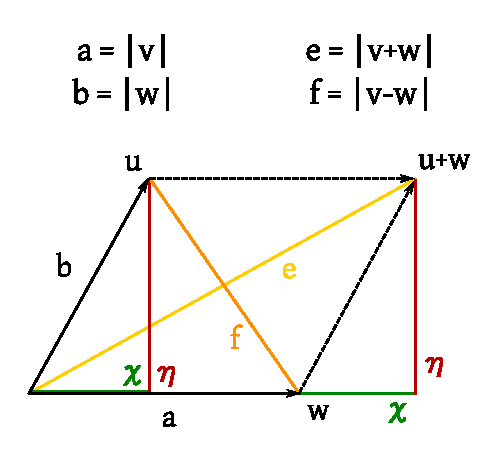
\includegraphics{img/parallelogram_norms.pdf}
          \caption{Norm addition illustrated in a parallelogram}
          \label{img:norm-parallelogram}
        \end{center}
      \end{figure}

      Compare with Figure~\ref{img:norm-parallelogram}.
      \[ \xi^2 + \eta^2 = b^2 \]
      \[ (a + \xi)^2 + \eta^2 = e^2 \]
      \[ (a - \xi)^2 + \eta^2 = f^2 \]
      \[ \underbrace{(a + \xi)^2 + (a - \xi)^2}_{2(a^2 + \xi^2 + \eta^2) = 2 (a^2 + b^2)} + 2\eta^2 = e^2 + f^2 \]
  \end{enumerate}
\end{theorem}

\begin{ex}[Counterexample]
  $\norm{x}_1 = \abs{x_1} + \ldots + \abs{x_n}$ does not satisfy the third property.
\end{ex}

\begin{rem}
  It is possible to show (von Neumann):
  If a norm satisfies the parallelogram equation,
  it originates from a scalar product.
\end{rem}

\index[English]{Orthogonal family}
\index[German]{\foreignlanguage{ngerman}{Orthogonale Familie}}
\index[English]{Orthonormal family}
\index[German]{\foreignlanguage{ngerman}{Orthonormale Familie}}
\index[English]{Orthonormal basis}
\index[German]{\foreignlanguage{ngerman}{Orthonormale Basis}}
\begin{defi}
  Let $(V, \langle, \rangle)$ be a vector space with scalar product.
  A family $(v_i)_{i \in I} \subseteq V$ is called
  \begin{description}
    \item[orthogonal] if $\bigwedge_{i\neq j} \functional{v_i, v_j} = 0$
    \item[orthonormal] if $\bigwedge_{i,j} \functional{v_i, v_j} = \delta_{ij} = \begin{cases} 0 & i \neq j \\ 1 & i = j \end{cases}$
    \item[orthonormal basis] if it is a basis and orthonormal
  \end{description}
\end{defi}

\index[English]{Trigonometric polynomials}
\index[German]{\foreignlanguage{ngerman}{Trigonometrische Polynome}}
\begin{ex}
  $(e_1, \ldots, e_n)$ in $\mathbb K^n$ is orthonormal basis in regards of the standard scalar product.
  \begin{enumerate}
    \item $\functional{e_i, e_j} = \delta_{ij}$
    \item
      \[ \int_0^1 \sin(2\pi mx) \sin(2\pi nx) \, dx = \delta_{mn} \cdot 2 \]
      \[ \int_0^1 \sin(2\pi nx) \cos(2\pi nx) \, dx = 0\]
      \[ \int_0^1 \cos(2\pi mx) \cos(2\pi nx) \, dx = \delta_{mn} \cdot 2 \]
      \[ \set{1} \cup \setdef{\frac{\sin(2\pi nx)}{\sqrt2}}{n \in \mathbb N} \cup \setdef{\frac{\cos(2\pi nx)}{\sqrt{2}}}{n \in \mathbb N} \]
      where
      \[ \functional{f,g} = \int_0^1 f(x) g(x) \, dx \]
      is orthonormal in $C[0,1]$.

      This is the spanned linear subspace.

      The result are the so-called trigonometric polynomials.
      \[ f(x) = \sum_{n=0}^\infty a_n \cos(2\pi nx) + \sum_{n=1}^\infty b_n \sin(2\pi nx) \]
  \end{enumerate}
\end{ex}

\begin{theorem}
  \label{satz-8.38}
  Let $(v_i)_{i \in I} \subseteq V$, $v_i \neq 0$.
  \begin{enumerate}
    \item $(v_i)_{i \in I}$ is orthogonal $\Leftrightarrow \left(\frac{v_i}{\norm{v_i}}\right)_{i \in I}$ is orthonormal.
    \item If $(v_i)_{i \in I}$ is orthogonal, then $(v_i)_{i \in I}$ is linear independent.
  \end{enumerate}
\end{theorem}
\begin{proof}
  \begin{enumerate}
    \item trivial
    \item Let $\lambda_1, \ldots, \lambda_n \in \mathbb K$ and $\lambda_1 v_{i_1} + \ldots + \lambda_k v_{i_k} = 0$,
      then all $\lambda_j = 0$.
      \begin{align*}
        0
        &= \functional{0, v_{ij}} \\
        &= \functional{\lambda_1 v_{i_1} + \ldots + \lambda_k v_{i_k}, v_{ij}} \\
        &= \lambda_1 \functional{v_{i_1}, v_{ij}} + \lambda_2 \functional{v_{i_2}, v_{ij}} + \ldots + \lambda_k \functional{v_{i_k}, v_{i_j}}
        &= \lambda_j \norm{v_{ij}}^2 \\
        &\Rightarrow \lambda_j = 0 \qquad \text{ for } j = 1, \ldots, k
      \end{align*}
  \end{enumerate}
\end{proof}

\begin{theorem}
  \label{satz-8.39}
  Let $B = (b_1, \ldots, b_n)$ be a orthonormal basis (ONB)
  of a finite-dimensional vector space $V$ over $\mathbb K$.
  Let $v,w \in V$ with
  \[
    \Phi_B(v) = \begin{pmatrix} \lambda_1 \\ \vdots \\ \lambda_n \end{pmatrix}
    \qquad
    \Phi_B(w) = \begin{pmatrix} \mu_1 \\ \vdots \\ \mu_n \end{pmatrix}
  \]
  Then it holds that
  \begin{enumerate}
    \item $\bigwedge_{i \in \set{1,\ldots,n}} \lambda_i = \functional{v,b_i}$
    \item $\functional{v,w} = \sum_{i=1}^n \lambda_i \overline{\mu_i}$
  \end{enumerate}
\end{theorem}
\begin{proof}
  \begin{enumerate}
    \item $\functional{v,b_i} = \functional{\sum_{j=1}^n \lambda_j b_j, b_i} = \sum_{j=1}^n \lambda_j \functional{\underbrace{b_j, b_i}_{\delta_{ji}}} = \lambda_i$
    \item
      \[
        \functional{v,w} = \Phi_B(v)^t A \overline{\Phi_B(w)} = \Phi_B(v)^t \overline{\Phi_B(w)} = \sum_{i=1}^n \lambda_i \overline{\mu_i}
      \] \[
        a_{ij} = \functional{b_i, b_j} = \delta_{ij}
      \]
  \end{enumerate}
\end{proof}

\index[English]{Orthogonal complement}
\index[German]{\foreignlanguage{ngerman}{Orthogonales Komplement}}
\begin{defi}
  \label{defi-8.40}
  $(V, \langle, \rangle)$. $M \subseteq V$ be a subset.
  Then
  \[ M^\bot \coloneqq \setdef{v \in V}{\bigwedge_{u \in M} \functional{v,u} = 0} \]
  is called \emph{orthogonal complement} of $M$. For $v \in V$, let $v^\bot \coloneqq \set{v}^\bot$.
\end{defi}

\begin{theorem}
  \label{satz-8.41}
  Let $(V, \langle, \rangle)$ and $M,N \subseteq V$.
  \begin{enumerate}
    \item $M^\bot$ is a subspace.
    \item $M \subseteq N \Rightarrow N^\bot \subseteq M^\bot$.
      \[ (M_1 \cup M_2)^\bot = M_1^\bot \cap M_2^\bot \]
    \item $\set{0}^\bot = V$
    \item $V^\bot = \set{0}$
    \item $M \cap M^\bot \subseteq \set{0}$
    \item $M^\bot = \mathcal L(M)^\bot$
    \item $M \subseteq (M^\bot)^\bot$
  \end{enumerate}
\end{theorem}
\begin{proof}
  \begin{enumerate}
    \item
      \[ u^\bot = \setdef{v}{\functional{v,u} = 0} \]
      \[ T_u: \substack{V \to \mathbb K \\ v \mapsto \functional{v,u}} \text{ is linear} \]
      \[ \setdef{v}{\functional{v,u} = 0} = \setdef{v}{T_u(v) = 0} = \kernel{T_u} \text{ is subspace} \]
      \[ M^\bot = \bigcap_{u \in M} u^\bot \text{ is intersection of subspaces} \]
    \item
      \[ N^\bot = \bigcap_{u \in N} u^\bot \subseteq \bigcap_{u \in M} u^\bot = M^\bot \]
      \[
        (M_1 \cup M_2)^\bot
        = \bigcap_{u \in M_1 \cup M_2} u^\bot - \bigcap_{u \in M_1} u^\bot \cap \bigcap_{u \in M_2} u^\bot
        = M_1^\bot \cap M_2^\bot
      \]
    \item trivial
    \item
      \[ V^\bot = V \cap V^\bot = \set{0} \]
    \item $v \in M \cap M^\bot \Rightarrow \functional{v,v} = 0 \Rightarrow v = 0$
    \item
      \[ \mathcal L(M)^\bot \subseteq M^\bot \qquad \text{ (because of 2.)} \]
      Show that: $M^\bot \subseteq \mathcal L(M)^\bot$: Let $v \in M^\bot$, $u \in \mathcal L(M)$
      Then
      \[ \exists u_1, \ldots, u_n \in M \exists \lambda_1, \ldots, \lambda_n \in \mathbb K:
        u = \lambda_1 u_1 + \ldots + \lambda_n u_n \]
      \[
        \Rightarrow \functional{v,u} = \functional{v,\sum_{i=1}^n \lambda_i u_i}
        = \sum_{i=1}^n \overline{\lambda_i} \functional{v, u_i} = 0
      \]
    \item
      Show: Let $v \in M$, then $\bigwedge_{u \in M^\bot} \functional{v,u} = 0$

      \[ \bigwedge_{u \in M^\bot} \functional{v,u} = \bigwedge_{u \in M^\bot} \functional{u,v} = 0 \]
  \end{enumerate}
\end{proof}

\meta{lecture}{20th of April 2016}{Franz Lehner}

\begin{theorem}
  Let $M^\bot = \setdef{v}{\bigwedge_{u \in M} u \bot v}$ is subspace.

  \begin{itemize}
    \item[6.] $M^\bot = L(M)^\bot$
    \item[2.] $M \subseteq N \Rightarrow N^\bot \subseteq M^\bot$
    \item[3.] $0^\bot = V$
    \item[4.] $V^\bot = \set{0}$
    \item[5.] $M \cap M^\bot \subseteq \set{0}$
  \end{itemize}
  \[ M \subseteq (M^\bot)^\bot \]
\end{theorem}

\begin{cor}
  \label{folderung-8.42}
  If $U \subseteq V$ is a subspace of $V$, then the sum $U + U^\bot$ is direct.
  \[ (U + U^\bot)^\bot \overset{\text{6.}}{=} (U \cup U^\bot)^\bot = U^\bot \cap (U^\bot)^\bot \overset{5.}{=} \set{0} \]
\end{cor}

From $(U + U^\bot)^\bot = \set{0}$, $U + U^\bot = V$ follows only in finite dimensions.

\begin{ex}
  \[ V = e^2 = \setdef{(\xi_n)_n}{\sum_{n=1}^\infty \abs{\xi_n}^2 < \infty} \]
  \[ U = \mathcal L((e_i)_{i \in \mathbb N}) \neq V = \setdef{(\xi_n)_n}{\xi_n = 0 \text{ for almost all } n} \]
  \[ U^\bot = \setdef{x = (\xi_n)_{n \in \mathbb N}}{\underbrace{\functional{x, e_i}}_{=\xi_i} = 0 \forall i} = \set{0} \]
  \[ V = (U^\bot)^\bot \neq U \qquad U = U + U^\bot \neq V, U^\bot = \set{0} \]
\end{ex}

Practicals:
\[ U + U^\bot = V \Leftrightarrow U = (U^\bot)^\bot \]

In the following we always assume: $V = U \dot{+} U^\bot$.

$\rightarrow$ projection: every vector has a unique decomposition.
\[ x = u + v \]
\[ u \in U \qquad v \in U^\bot \text{ such that } u \bot v \]

\index[English]{Convex set}
\index[German]{\foreignlanguage{ngerman}{Konvexe Menge}}
\begin{defi}
  \label{defi-8.44}
  Let $V$ be a vector space.
  A subset $K \subseteq V$ is called convex if
  \[ \bigwedge_{x,y \in \mathbb K} \bigwedge_{\lambda \in [0,1]} x + \lambda (y - x) \in \mathbb K \]
  $(1 - \lambda) x + \lambda y$ is called \emph{convex combination}.

  Informally: A set is convex if all elements of the path between two points of the set
  are inside the set.
\end{defi}

\begin{ex}
  \label{bsp-8.45}
  \begin{enumerate}
    \item Let $(V, \norm{ })$ be a normed space. Then
      \[ B(0,1) - \setdef{x}{\norm{x} < 1} \text{ is convex} \]
      \[ x,y \in B(0,1), \lambda \in [0,1]: \norm{(1 - \lambda) x + \lambda y} \leq (1 - \lambda) \norm{x} + \lambda \norm{y} < (1 - \lambda) + \lambda > 1 \]
    \item Subspaces are convex.
    \item Translations and scalar multiples of convex sets are convex
      \begin{itemize}
        \item Linear manifolds
        \item $B(\times, r)$ is convex.
      \end{itemize}
    \item $K \subseteq V$ is convex, $f: V \to W$ is linear $\Rightarrow f(\mathbb K)$ is convex (the proof is left as an exercise  ).
  \end{enumerate}
\end{ex}

\begin{rem}
  What does optimization mean?

  Given an audio file with data. We want to approximate these data, but the maximum size of the data is defined.
  So we optimize the data such that the file size is decreased.

  Formally: Find $x \in K$ with $\norm{X} = \min$.
\end{rem}

\begin{rem}
  Consider $l^1: \norm{x} = \abs{x_1} \abs{x_2}$.
  The unit circle is a square rotated by $45^\circ$.

  If we expand this unit circle to our desired $K$ (a straight line like $f(x) = -x$),
  the intersection of $K$ and this expanded unit circle yields infinitely many points.
\end{rem}

\begin{theorem}
  \label{satz-8.46}
  Let $(V, \langle, \rangle)$ be a vector space with scalar product.
  $K \subseteq V$ is convex, $x \in V$, $y_0 \in K$.

  DFASÄ:
  \begin{enumerate}
    \item $\bigwedge_{y \in K} \norm{x - y_0} \leq \norm{x - y}$
    \item $\bigwedge_{y \in K} \Re\functional{x - y_0, y - y_0} \leq 0$
    \item $\bigwedge_{y \in K \setminus \set{y_0}} \norm{x - y_0} < \norm{x - y}$
  \end{enumerate}
\end{theorem}

\begin{rem}
  If $K$ is a linear manifold, then (2.) is equivalent to:
  \begin{enumerate}
    \item[2'.] $\bigwedge_{y \in K} \functional{x - y_0, y - y_0} = 0$
  \end{enumerate}
\end{rem}

\begin{proof}
  \begin{description}
    \item[1. $\rightarrow$ 2.]
      Let $y \in K$. $0 < \varepsilon < 1$. Compare with Figure~\ref{img:norm}.
      \begin{figure}[!h]
        \begin{center}
          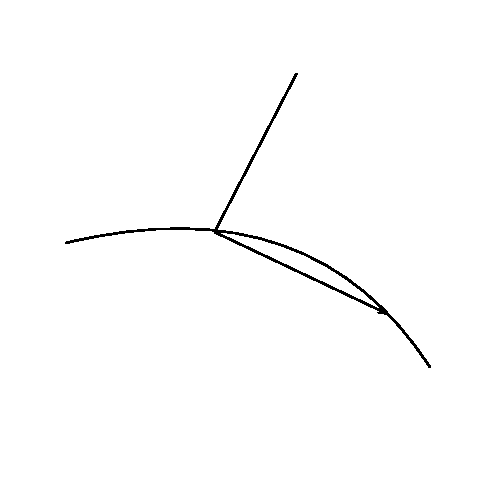
\includegraphics{img/norm.pdf}
          \caption{Norm}
          \label{img:norm}
        \end{center}
      \end{figure}
      \[ \Rightarrow y_\varepsilon = (1 - \varepsilon) y_0 + \varepsilon y_1 \in K \]
      \[ \Rightarrow \norm{x - y_0} \leq \norm{x - y_\varepsilon} \]
      \[ y_\varepsilon = y_0 + \varepsilon (y - y_0) \]
      \begin{align*}
        0 &\leq \norm{x - y_\varepsilon}^2 - \norm{x - y_0}^2 \\
          &= \norm{x - y_0 - \varepsilon (y - y_0)}^2 - \norm{x - y_0}^2 \\
          &= \norm{x - y_0}^2 + \varepsilon^2 \norm{y - y_0}^2 - 2 \Re{\functional{x - y_0, y - y_0}} \varepsilon - \norm{x - y_0}^2 \\
          &= \varepsilon(\varepsilon \norm{y - y_0}^2 - 2 \Re{\functional{x - y_0, y - y_0}}) \\
        \varepsilon \to 0 & \Rightarrow -2 \Re{\functional{x - y_0, y - y_0}} \geq 0
      \end{align*}
      If $\Re{x - y_0, y - y_0} > 0$, then $y \neq y_0$. Choose
      \[ \varepsilon < \frac{2\Re{\functional{x - y_0, y - y_0}}}{\norm{y - y_0}} \]
      This leads to a contradiction.
    \item[2. $\rightarrow$ 3.]
      Let $y \in K \setminus \set{y_0}$.
      \begin{align*}
        \norm{x - y}^2 &= \norm{x - y_0 - (y - y_0)}^2 \\
          &= \norm{x - y_0}^2 + \norm{y_0 - y}^2 - 2 \Re{\functional{x - y_0, y - y_0}} \\
          &\geq \norm{x - y_0^2} + \norm{y_0 - y}^2 \\
          &> \norm{x - y_0}^2
      \end{align*}
    \item[3. $\rightarrow$ 1.]
      trivial
  \end{description}

  If $K = U$ is a subspace.
  \begin{enumerate}
    \item[2.]
    \[ y - y_0 \in U \Leftrightarrow y \in U \]
      \begin{align*}
        \bigwedge_{y \in U} \Re{\functional{x - y_0, \underbrace{y - y_0}_{\eqqcolon z \in U}}} &\leq 0 \\
        \Leftrightarrow \bigwedge_{z \in U} \Re{\functional{x - y_0, z}} &\leq 0 \\
        \Rightarrow \bigwedge_{z \in U} \Re{\functional{x - y_0, -z}} &\leq 0 \\
        \Leftrightarrow \bigwedge_{z \in U} \Re{\functional{x - y_0, z}} &\geq 0 \\
        \Rightarrow \bigwedge_{z \in U} \Re{\functional{x - y_0, z}} &= 0 \\
        \Rightarrow \bigwedge_{z \in U} \Re{\functional{x - y_0, iz}} &= 0 \\
        \Rightarrow \bigwedge_{z \in U} \Re{(-i \functional{x - y_0, z})} &= 0
      \end{align*}
      \[ \Re(-i (a + ib)) = b \]
      \[ \Rightarrow \bigwedge_{z \in U} \Im\functional{x - y_0, z} = 0 \]
      \[ \Rightarrow \bigwedge_{z \in U} \functional{x - y_0, z} = 0 \Rightarrow x - y_0 \in U^\bot \]
  \end{enumerate}
\end{proof}

\begin{cor}
  Let $(V, \langle, \rangle)$ be a vector space with a scalar product.
  \begin{enumerate}
    \item If $K \subseteq V$ is convex, then the optimization problem
      \[
        \left\{
          \begin{array}{c}
            \norm{x - y} = \text{min!} \\
            y \in K
          \end{array}
        \right.
      \]
      has at most one solution.
    \item If $U \subseteq V$ is a subspace, $x \in V$, then there exists at most
      one point $y_0 \in U$ such that $x - y_0 \in U^\bot$.

      $\Rightarrow$ the sum $U + U^\bot$ is direct.
  \end{enumerate}
\end{cor}

\index[English]{Orthogonal projections}
\index[German]{\foreignlanguage{ngerman}{Orthogonalprojektionen}}
\begin{defi}
  Let $(V, \langle, \rangle)$ is a vector space with scalar product.
  Let $U \subseteq V$ a subspace with $V = U \dot{+} U^\bot$.

  Let's recognize that
  \[ V = U \dot{+} W \]
  \[ \bigwedge_{x} \bigvee_{\substack{u \in U \\ w \in W}} = u + w \]

  Then $\pi_U: V \to V$ and $\pi_{U^\bot}: V \to V$ such that
  \[ \bigwedge_{x \in V} \pi_U(x) \in U \land \pi_{U^\bot}(x) \in U^\bot \]
  are called \emph{orthogonal projections} to $U$ and $U^\bot$.

  Compare with Figure~\ref{img:orth-proj}.
\end{defi}

\begin{figure}[!h]
  \begin{center}
    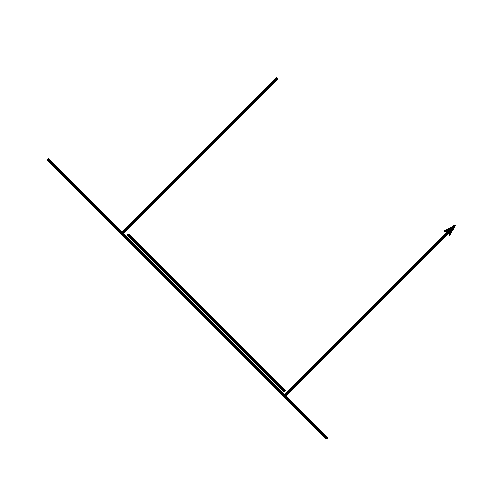
\includegraphics{img/orthogonal_projections.pdf}
    \caption{Orthogonal projections}
    \label{img:orth-proj}
  \end{center}
\end{figure}

\begin{theorem}[Revision of direct sums of vector spaces]
  \label{wh-8.49}
  \begin{enumerate}
    \item $x \in U \Leftrightarrow \pi_U(x) = x \Leftrightarrow \pi_{U^{\bot}}(x) = 0$
    \item $x \in U^{\bot} \Leftrightarrow \pi_U(x) = 0 \Leftrightarrow \pi_{U^{\bot}}(x) = x$
    \item $\pi_{U^{\bot}} = \text{id} - \pi_U$
    \item $\pi_U \circ \pi_U = \pi_U$
    \item $\pi_U$ is linear
  \end{enumerate}
\end{theorem}

\begin{theorem}
  \label{satz-8.50}
  Let $V = U \dot{+} U^{\bot}$.
  \begin{enumerate}
    \item $\bigwedge_{x,y \in V} \functional{x, \pi_U(y)} = \functional{\pi_U(x), y} = \functional{\pi_U(x), \pi_U(y)}$
    \item $\bigwedge_{x \in V} \norm{\pi_U(x)} \leq \norm{x}$
      and $\norm{\pi_U(x)} = \norm{X} \Leftrightarrow x \in U$
  \end{enumerate}
\end{theorem}

\begin{proof}
  \begin{enumerate}
    \item
      \begin{align*}
        x &= \pi_U(x) + \pi^{U^\bot}(x) \\
        y &= \pi_U(y) + \pi_{U^\bot}(y) \\
        \functional{x, \pi_U(y)} &= \functional{\pi_U(x) + \pi_{U^{\bot}}(x), \pi_U(y)} \\
          &= \functional{\pi_U(x), \pi_U(y)} + \functional{\underbrace{\pi_{U^\bot}(x)}_{\in U^\bot}, \underbrace{\pi_U(y)}_{\in U}} \\
        \functional{\pi_U(x), y} &= \functional{\pi_U(x), \pi_U(y)}
      \end{align*}
    \item
      \begin{align*}
        \norm{x}^2 &= \norm{\pi_U(x) + \pi_{U^\bot}(x)}^2 \\
        \text{Pythagorean theorem} &= \norm{\pi_U(x)}^2 + \norm{\pi_{U^\bot}(x)}^2 \\
          &\geq \norm{\pi_U(x)}^2 \\
        \text{equality} &\Leftrightarrow \pi_{U^\bot}(x) = 0 \Leftrightarrow x \in U
      \end{align*}
  \end{enumerate}
\end{proof}

\begin{defi}
  \label{defi-8.51}
  J\o rgen Pedersen Gram (1850--1916)

  Let $(V, \langle, \rangle)$ is a vector space with scalar product.
  Let $v_1, \ldots, v_m \in V$.

  Then the matrix is called
  \[
    \operatorname{Gram}(v_1, \ldots, v_m)
    \coloneqq \begin{bmatrix}
      \functional{v_1, v_1} & \functional{v_1, v_2} & \ldots & \functional{v_1, v_m} \\
      \functional{v_2, v_1} & \functional{v_2, v_2} & \ldots & \functional{v_2, v_m} \\
      \vdots & \vdots & \ddots & \vdots \\
      \functional{v_m, v_1} & \functional{v_m, v_2} & \ldots & \functional{v_m, v_m} \\
    \end{bmatrix}
    \in \mathbb K^{m \times m}
  \]
  \emph{Gram's matrix of tuple} $(v_1, \ldots, v_m)$
\end{defi}

\begin{rem}
  \[ V = \mathbb R^n \qquad (\mathbb C^n) \]
  \[ \functional{v_i, v_j} = v_i^t v_j \]
  \[ \leadsto G = V^t \overline{V} \]
  \[
    V = \begin{pmatrix}
      V_1 & V_2 & \ldots & V_m \\
      \vdots & \vdots &  & \vdots
    \end{pmatrix}
  \]
\end{rem}

\begin{theorem}
  \label{satz-8.53}
  Let $(V, \langle, \rangle)$ be a vector space with a scalar product.
  $v_1, \ldots, v_m \in V$.
  \begin{enumerate}
    \item
      $G = \operatorname{Gram}(v_1, \ldots, v_m)$ is hermitian and positive semidefinite.
      Furthermore it holds that
      \[ \xi^t \cdot G \cdot \overline{\xi} = \norm{\sum_{i=1}^m \xi_i v_i}^2 \]
    \item
      \[ \xi \in \kernel(G) \Leftrightarrow \sum_{i=1}^m \overline{\xi_i} v_i = 0 \]
    \item
      $G$ is positive definite iff $G$ is regular iff $v_1, \ldots, v_m$ are linear independent.
  \end{enumerate}
\end{theorem}

\begin{proof}
  \begin{enumerate}
    \item
      \[ g_{ij} = \functional{v_i, v_j} = \overline{\functional{v_j, v_i}} = \overline{g_{ji}} \]
      $\Rightarrow$ G is Hermitian.

      \begin{align*}
        \xi^t G \overline{\xi} &= \sum_{i,j=1}^m \xi_i \functional{v_i, v_j} \overline{\xi_j} \\
          &= \functional{\sum_{i=1}^m \xi_i v_i, \sum_{j=1}^m \xi_j v_j} \\
          &= \norm{\sum_{i=1}^m \xi_i v_i}^2
      \end{align*}
    \item $\Rightarrow$
      Let $\xi \in \kernel{G}$.
      \[ G \cdot \xi = 0 \Rightarrow \underbrace{\overline{\xi}^t G \xi}_{= \norm{\sum \overline{\xi_i v_i}}^2} = 0 \]
      \[ \Rightarrow \sum_{i=1}^m \overline{\xi_i} v_i = 0 \]

      $\Leftarrow$
      Let $\sum_{i=1}^m \xi_i v_i = 0$.
      \[
        (G \cdot \xi)_i = \sum_{j=1}^m \functional{v_i, v_j} \xi_j
        = \functional{v_i, \underbrace{\sum_{j=1}^m \overline{\xi_j}}_{=0} v_j} = 0
      \]
      holds for all $i = 1,\ldots,m$.
      \[ \Rightarrow G \cdot \xi = 0 \Rightarrow \xi \in \kernel{G} \]
    \item
      \begin{align*}
        G > 0 &\Leftrightarrow \xi^t G \overline{\xi} > 0 \quad \forall \xi \neq 0 \\
          &\Leftrightarrow \norm{\sum \xi_i v_i}^2 > 0 \quad \forall \xi \neq 0 \\
          &\Leftrightarrow \sum \xi_i v_i \neq 0 \quad \forall \xi \neq 0 \\
          &\Leftrightarrow v_1,\ldots,v_m \text{ is linear independent} \\
          &\Leftrightarrow \kernel{G} = \set{0} \\
          &\Leftrightarrow G \text{ regular}
      \end{align*}
  \end{enumerate}
\end{proof}

\meta{lecture}{25th of April 2016}{Franz Lehner}

Revision:
\begin{itemize}
  \item Approximation of a $x$ (outside) in a convex set by computing the orthogonal line from $x$ to the border of the convex set intersecting the set at $y_0$ ($\norm{x - y_0}$ min, $y_0 \in K$)
  \[ \bigwedge_{y \in K} \Re{\functional{x - y_0, y - y_0}} \leq 0 \]
  \item $u = \pi_u(x)$ is the unique element $u \in U$ such that $x-u \in U^\bot$. $U$ is defined such that $U \dot{+} U^\bot = V \Leftrightarrow U = (U^\bot)^\bot$. $\pi_U$ is linear.
\end{itemize}

\begin{theorem}
  \label{satz-8.53}
  Consider $v_1, \ldots, v_m \in V$.
  \[ \operatorname{Gram}(v_1, \ldots, v_m) = \left[\functional{v_2, v_1}\right]^m_{i,j=1} \]
  \[ \xi^t G \xi = \norm{\sum \xi_i v_i}^2 \]
  $G$ is positive definite iff $v_1, \ldots, v_m$ are linear independent.
\end{theorem}

\begin{theorem}
  \label{satz-8.54}
  Let ($V, \langle, \rangle$) be a vector space with scalar product.
  $U \subseteq V$ is subspace with $\dim{U} < \infty$.
  $(u_1, \ldots, u_n)$ is basis of $U$.
  $G = \operatorname{Gram}(u_1, \ldots, u_m)$ is positive definite and regular.
  Then the orthogonal projection to $U$ for $x \in V$ is given by
  \[ \pi_U(x) = \sum_{j=1}^m \eta_j u_j \]
  where $\overline{\eta} = G^{-1} \xi$.
  \[ \xi = \begin{pmatrix} \functional{x,u_1} \\ \vdots \\ \functional{x,u_m} \end{pmatrix} \]
  (wrt. claiming $u_1, \ldots, u_m$ is orthogonal normal basis and Gram matrix provides correction to achieve that)
\end{theorem}
\begin{proof}
  Let $u = \sum_{j=1}^m \eta_j u_j$. Because
  \[ \bigwedge_{y \in U} \functional{x - y_0, y - y_0} = 0 \]
  holds, it holds that $x - u \in U^\bot = \underbrace{\set{u_1, \ldots, u_m}}_{\text{basis of } U'}^\bot$.

  Hence we need to show:
  \[ \functional{u_i, u} = \functional{u_i, x} \qquad \text{ for } i = 1, \ldots, m \]
  \[ \functional{u_i, u} = \functional{u_i, \sum_{j=1}^m \eta_j u_j} = \sum_{j=1}^m \underbrace{\functional{u_i, u_j}}_{= G_{ij}} \overline{\eta}_j \]
  \[ = (G \overline{\eta})_i = \overline{\xi}_i = \overline{\functional{x_i, u_i}} = \functional{u_i, x} \]
  \[ \Rightarrow \functional{x - u, u_i} = 0 \quad \forall i \]
  \[ \Rightarrow x-u \in U^\bot \]
\end{proof}

\index[English]{Hilbert matrix}
\index[German]{\foreignlanguage{ngerman}{Hilbert Matrix}}
\index[English]{Hankel matrix}
\index[German]{\foreignlanguage{ngerman}{Hankel matrix}}
\begin{ex}
  \label{bsp-8.55}
  Determine the polynomial $p(x)$ of degree $\leq 2$ such that
  \[ \int_0^1 \abs{t^3 - p(t)}^2 \, dt = \text{ min!} \]
  where $V = \mathbb R[x]$ and $K = U = \mathbb R_2[x] = \mathcal{L}(1, x, x^2)$.
  \[ \functional{f,g} = \int_0^1 f(t) g(t) \, dt \]

  Find: Orthogonal projection of $x^3$ to $\mathcal L(1, x, x^2)$

  \begin{description}
    \item[Step 1: Gram matrix $G$]
      \[
        G_{ij}
        = \int_0^1 t^{i-1} t^{j-1} \, dt
        = \int_0^1 t^{i+j-2} \, dt
        = \frac{1}{i + j - 1}
      \] \[
        G = \begin{bmatrix}
          1 & \frac12 & \frac13 \\
          \frac12 & \frac13 & \frac14 \\
          \frac13 & \frac14 & \frac15
        \end{bmatrix}
        \qquad \text{\enquote{Hilbert matrix}}
      \]
      Hankel matrix:
        $a_{ij}  a_{i'j'}$ if $i + j = i' + j'$
      \[
        \begin{pmatrix}
          h_1 & h_2 & h_3 & \ldots \\
          h_2 & h_3 & h_4 & \ldots \\
          h_3 & h_4 & h_5 & \ldots
          \vdots & & &
        \end{pmatrix}
      \]
      \enquote{momentum problem}  % dt. Momentenproblem

      Our solution:
      \[ p(t) = \sum_{i=1}^3 \eta_i t^{i-1} \]
      \[ \eta = G^{-1} \xi \qquad \xi_i = \functional{x^3, u_i} = \int_0^1 t^3 t^{i-1} \, dt = \frac{1}{3+i} \]
      \[
        \eta = \begin{bmatrix}
          1 & \frac12 & \frac13 \\
          \frac12 & \frac13 & \frac14 \\
          \frac13 & \frac14 & \frac15
        \end{bmatrix}^{-1}
        \begin{bmatrix} \frac14 \\ \frac15 \\ \frac16 \end{bmatrix}
        = \begin{bmatrix}
          9 & -36 & 30 \\
          -36 & 192 & -180 \\
          30 & -180 & 180
        \end{bmatrix}
        \begin{bmatrix} \frac14 \\ \frac15 \\ \frac16 \end{bmatrix}
        = \begin{bmatrix} -\frac1{20} \\ -\frac35 \\ \frac32 \end{bmatrix}
      \]
      Solution:
      \[ p(x) = \frac1{20} - \frac35 x + \frac32 x^2 \]

      $n\times n$ Hilbert matrix:
      \[ \det{H_n} = \frac{c_n^4}{c_{2n}} \sim \frac{(2\pi)^{\overbrace{l_n}^{\text{Stirling}}}}{4^{n^2} \sqrt[4]{n}} \]
      \[ c_n = \prod_{i=1}^{n-1} i! \]

      \enquote{Almost} not invertible.
      So this matrix is actually a good test matrix for numerical algorithms.
  \end{description}
\end{ex}

\index[English]{Bessel's inequality}
\index[German]{\foreignlanguage{ngerman}{Besselsche Ungleichung}}
\begin{cor}
  \label{korollar-8.56}
  Let $U \subseteq V$ be a subspace and $(u_1, \ldots, u_m)$ be an orthonormal basis.
  Then it holds that
  \begin{itemize}
    \item $\bigwedge_{v \in V} \pi_u(v) = \sum_{i=1}^m \functional{v, u_i} u_i$
    \item
      $\bigwedge_{v \in V} \sum_{i=1}^m \abs{\functional{v, u_i}}^2 \leq \norm{v}^2$,
      \quad \enquote{Bessel's inequality} \\
      $\bigwedge_{v \in V} \sum_{i=1}^m \abs{\functional{v, u_i}}^2 = \norm{v}^2 \Leftrightarrow v \in U$,
      \quad \enquote{Parseval's identity}
  \end{itemize}
\end{cor}
\begin{proof}
  Immediate.
  $G = I$, hence $\eta_i = \xi_i$.
\end{proof}

\begin{rem}
  So if $u_1, \ldots, u_m$ is an orthonormal basis of $U$,
  then we can immediately determine $\pi_U(v)$.
  Can we fine an orthonormal basis?
\end{rem}

\index[English]{Gram-Schmidt process}
\index[German]{\foreignlanguage{ngerman}{Gram-Schmidt Orthogonalisierungsverfahren}}
\begin{theorem}[Gram–Schmidt process]
  \label{satz-8.57}
  Given $v_1, \ldots, v_m$ is linear independent.
  Determine orthonormal system $u_1, \ldots, u_m$
  such that $\mathcal L(u_1, \ldots, u_m) = \mathcal L(v_1, \ldots, v_m)$.

  Let ($V, \langle, \rangle$) be vector space with scalar product.
  Let $(v_1, \ldots, v_n)$ be linear independent.

  Then there exists a orthonormal system $(u_1, \ldots, u_m) \subseteq V$
  such that $\mathcal L(u_1, \ldots, u_m) = \mathcal L(v_1, \ldots, v_m)$.
  Find $u \in U_k$ such that $v_{k+1} - u \in U_k^\bot$.

  Inductively,
  \[ u_1 = \frac{v_1}{\norm{v_1}} \qquad U_k = \mathcal L(v_1, \ldots, v_k) = \mathcal L(u_1, \ldots, u_k) \]
  and for $k=2, \ldots, m$:
  Let
  \[ \tilde{u_k} = v_k - \underbrace{\sum_{j=1}^{k-1} \functional{v_k, u_j} u_j}_{\pi_{U_{k-1}}(v_k)} \]
  \[ U_k = \frac{\tilde{U_k}}{\norm{\tilde{U_k}}} \]
\end{theorem}
\begin{proof}
  \begin{description}
    \item[Case $k=1$]
      $v_1 \neq 0$ because they are linear independent.
      \[ \rightarrow u_1 = \frac{v_1}{\norm{v_1}} \]
    \item[Case $k-1\to k$]
      $u_1,\ldots,u_{k-1}$ is orthonormal sysm with $\mathcal L(u_1, \ldots, u_{k-1}) = \mathcal L(v_1, \ldots, v_{k-1})$.
      $v_k \not\in \mathcal L(u_1, \ldots, u_{k-1}) \eqqcolon U_{k-1}$.

      \begin{align*}
        \tilde{u_k} &= v_k - \sum_{j=1}^{k-1} \functional{v_k, u_j} u_j \\
          &\overset{\text{Theorem~\ref{satz-8.56}}}{=} v_k - \pi_{U_{k-1}}(v_k) \in U_{k-1}^\bot \\
          &\Rightarrow \tilde{u_k} \bot u_1, \ldots, u_{k-1}, \tilde{u_k} \neq 0 \text{ because } v_k \text{ is linear independent of } u_1, \ldots, u_{k-1} \\
        u_k &= \frac{\tilde{u_k}}{\norm{\tilde{u_k}}} \to (u_1, \ldots, u_k) \text{ is an orthonormal system}
      \end{align*}

      Immediate:
      \[ \tilde{u_k} \in \mathcal L(u_1, \ldots, u_{k-1}, u_k) = \mathcal L(v_1, \ldots, v_k) \]
      \[ v_k = \tilde{u_k} + \sum \lambda_j u_j \in \mathcal L(u_1, \ldots, u_{k-1}, \tilde{u_k}) = \mathcal L(u_1, \ldots, u_k) \]
  \end{description}
\end{proof}

\begin{ex}
  Let $V = \mathbb R^3$ with an inner product.
  \[ \functional{x,y} = x^t A y \text{ with } A = \begin{pmatrix} 1 & -1 & 1 \\ -1 & 3 & -1 \\ 1 & -1 & 2 \end{pmatrix} \]
  Find an orthonormal basis.

  \begin{enumerate}
    \item We orthogonalize the canonical basis $e_1, e_2$ and $e_3$.
    \[
      v_1 = \begin{pmatrix} 1 \\ 0 \\ 0 \end{pmatrix}
      \qquad \norm{v_1} = v_1^t A v_1 = 1
    \] \[
      u_1 = \begin{pmatrix} 1 & 0 & 0 \end{pmatrix}
    \]
    \[
      v_2 = \begin{pmatrix} 0 \\ 1 \\ 0 \end{pmatrix}
      \qquad
      \tilde{u_2} = v_2 - \overbrace{\functional{v_2, u_1}}^{=a_{21}} u_1
      = \begin{pmatrix} 0 \\ 1 \\ 0 \end{pmatrix} - (-1) \cdot
      \begin{pmatrix} 1 \\ 0 \\ 0 \end{pmatrix} = \begin{pmatrix} 1 \\ 1 \\ 0 \end{pmatrix}
    \] \[
      \functional{u_1, \tilde{u_2}} = 0
    \] \[
      \norm{\tilde{u}_2}^2 = \begin{pmatrix} 1 & 1 & 0 \end{pmatrix} A \begin{pmatrix} 1 \\ 1 \\ 0 \end{pmatrix} = 1 - 1 - 1 + 3 = 2
    \] \[
      u_2 = \frac{1}{\sqrt{2}} \begin{pmatrix} 1 \\ 1 \\ 0 \end{pmatrix}
    \] \[
      v_3 = \begin{pmatrix} 0 \\ 0 \\ 1 \end{pmatrix}
    \] \[
      \tilde{u}_3 = v_3 - \functional{v_3, u_1} u_1 - \frac{\functional{v_3, \tilde{u}_2} \tilde{u}_2}{\norm{\tilde{u}_2}^2}
    \] \[
      = \begin{pmatrix} 0 \\ 0 \\ 1 \end{pmatrix} - 1 \begin{pmatrix} 1 \\ 0 \\ 0 \end{pmatrix} - 0 \cdot \tilde{u}_2 = \begin{pmatrix} -1 \\ 0 \\ 1 \end{pmatrix}
    \]
    Solution:
    \[
      \left(
        \begin{pmatrix} 1 \\ 0 \\ 0 \end{pmatrix},
        \frac{1}{\sqrt{2}} \begin{pmatrix} 1 \\ 1 \\ 0 \end{pmatrix},
        TODO
      \right)
    \]
  \end{enumerate}
\end{ex}

\begin{theorem}[Alternative approach to build an orthogonal projection (in $\mathcal C^n$)]
  \label{satz-8.59}
  Determine orthonormal basis ($u_1, \ldots, u_m$) of subspace $U \subseteq \mathcal C^n$, then
  \[ P = \sum_{i=1}^m u_i u_i^* = \sum_{i=1}^m u_i \overline{u_i^t} \]

  Hence given $v \in \mathbb C^n$,
  \[ P \cdot v = \sum_{i=1}^m u_i \underbrace{u_i^* v}_{= \functional{v, u_i}} \]
\end{theorem}

\begin{ex}
  Considering Exercise~\ref{bsp-8.55} again.
  \[ V = \mathbb R[x] \qquad U = \mathcal L(1, x, x^2) \]
  Orthonormal basis:
  \[ \norm{v_1}^2 = \int_0^1 1^2 \, dt = 1 \]
  \[ u_1 = 1 \]

  \begin{align*}
    \tilde{u}_2 &= v_2 - \functional{v_2, u_1} u_1 \\
      &= \left(\functional{x,1} = \int_0^1 t \cdot 1 \, dt = \frac12 \right) \\
      &= x - \functional{x, 1} \cdot 1 \\
      &= x - \frac12
  \end{align*}
  \[ \norm{\tilde{u}_2}^2 = \int_0^1 (t - \frac12)^2 \, dt = \left. \frac{(t - \frac12)^3}{3}\right|_0^1 = \frac1{12} \]
  \[ u_2 = \sqrt{12} \cdot \left(x - \frac12\right) \]

  \[ \tilde{u}_3 = x^2 - \functional{x^2,1} \cdot 1 - \functional{x^2, x - \frac12} \left(x - \frac12\right) \cdot 12 = x^2 - x + \frac16 \]
  \[ \norm{\tilde{u}_3}^2 = \int_0^1 \left(t^2 - t + \frac16\right)^2 \, dt = \frac{1}{180} \]
  \[
    \pi_U(x^3)
      = \functional{x^3, 1} \cdot 1
      + \functional{x^3, x-\frac12} \left(x - \frac12\right) \cdot 12
      + \functional{x^3, x^2 - x + \frac16} \left(x^2 - x + \frac16\right) \cdot 180
  \]
\end{ex}

\begin{rem}
  Let $V$ be a vector space with a scalar product. $\dim{V} < \infty$.
  \begin{itemize}
    \item Every subspace $U$ has a unique orthogonal complement $U^\bot$ such that $V = U \oplus U^\bot$.
    \item $\pi_U: V \to U$ is an orthogonal projection with the property:
      \[ \norm{\pi_U(v)} \leq \norm{v} \]
    \item We can determine an orthonormal basis of $U$, then
      \[ \pi_U(v) = \sum_{i=1}^n \functional{v, u_i} u_i \]
      $\Rightarrow$ Bessel's inequality
  \end{itemize}
\end{rem}

\begin{rem}[Revision]
  $\operatorname{Hom}(V, \mathbb K) = V^*$ dual space.
  The map
  \[ V \times V^* \to \mathbb K \]
  \[ (x, f) \mapsto \functional{f, x} = f(x) \]
  is bilinear.

  Consider scalar product:
  \[ V \times V \to \mathbb K \]
  \[ (x, y) \mapsto \functional{x, y} \]
  is sesquilinear.

  Every $y \in V$ induces $f_y \in V^*$, $f_y(x) = \functional{x, y}$.

  Consider:
  \[ V \to V^* \]
  \[ y \mapsto f_y \]
  is an anti-linear embedding.

  Why? Injectivity:
  $f_y = 0 \Rightarrow f_y(x) = 0 \quad \forall x$.
  Especially, $f_y(y) = \functional{y,y} = \norm{y}^2 = 0 \Rightarrow y = 0$.
\end{rem}

\begin{theorem}[Riesz representation theorem]
  Frigyes Riesz (1880--1956)
  Let ($V, \langle, \rangle$) is vector space with scalar product.
  $\dim{V} < \infty$.

  Then the map
  \[ V \to V^* \]
  \[ y \mapsto f_y: V \to \mathbb K \text{ with } x \mapsto \functional{x,y} \]
  is an antilinear isomorphism.
\end{theorem}
\begin{proof}
  Injectivity has already been shown.
\end{proof}

\meta{lecture}{27th of April 2016}{Franz Lehner}

\begin{rem}[Revision]
  \[ U \subseteq V \]

  How to determine $\pi_U: V \to U$? Gram-Schmidt process or construct orthonormal basis
  $(u_1, u_2, \ldots, u_n)$ with $\pi_u(v) = \sum_{i=1}^m \functional{v_i u_i} u_i$
  \[ \norm{\pi_u(v)} \leq \norm{v} \]
  \[ \sum_{i=1}^{w} \abs{\functional{v_i, u_i}}^2 \leq \norm{v}^2 \]
  Bessel or equivalently $v \in U$ Parseval (*1755)
\end{rem}

\begin{theorem}
  \[ V^* = \Hom(V, \mathbb K) \overset{\sim}{-} V \]
  The map $V \to V^*$ with $y \mapsto f_y: V \to \mathbb K$ with $x \mapsto \functional{x,y}$
  is anti-linear\footnote{In $\mathbb R$ linear, in $\mathbb C$ it does make a difference} and bijective.

  \[ f_{\lambda y + \mu z} = \overline{\lambda} f_y + \overline{\mu} f_z \]
\end{theorem}

\begin{rem}
  We have already shown that $y \mapsto f_y$ is injective.
\end{rem}
\begin{rem}[Surjectivity]
  Given $f \in V^*$. Find $y \in V$ such that $f = f_y$.
\end{rem}

\begin{theorem}
  Let $(u_1, \ldots, u_n)$ be an orthonormal basis of $V$.
  Let $y = \sum_{i=1}^n \overline{f(u_i)} u_i$.
  \begin{align*}
    f_y(x) &= \functional{x,y} = \functional{x, \sum_{i=1}^n \overline{f(u_i)} u_i} \\
      &= \sum_{i=1}^n f(u_i) \functional{x,u_i} \\
      &= f\left(\sum_{i=1}^n \functional{x,u_i} u_i\right) \\
      &= f(x) \\
    \Rightarrow f_y &= f
  \end{align*}
\end{theorem}

\begin{theorem}[Second Riesz representation theorem]
  \[ C[0,1]^* = \text{ space of measures in } [0,1] \]
\end{theorem}
\begin{proof}
  The proof would take about 4 months of lectures.
\end{proof}

\begin{ex}
  \label{ex-8.62}
  \begin{itemize}
    \item
      \begin{align*}
        v = 0 &\Leftrightarrow \bigwedge_{w \in V} \functional{v,w} = 0 \\
              &\Leftrightarrow \bigwedge_{f \in V^*} f(v) = 0
      \end{align*}
      or
      \[ v_1 = v_2 \Leftrightarrow \bigwedge_{w \in V} \functional{v_1, w} = \functional{v_2, w} \]
    \item
      \begin{align*}
        \norm{v} = \sqrt{\functional{v,v}}
          &= \sup\setdef{\abs{\functional{v,w}}}{\norm{w} \leq 1} \\
          &= \sup\setdef{\abs{f(v)}}{f \in V^*, \norm{f} \leq 1}
      \end{align*}
  \end{itemize}
\end{ex}

\begin{rem}[Reminder]
  \[ f \in \Hom(V,W) \qquad f: V \overset{f}{\to} W \overset{w^*}{\to} \mathbb K \]
  \[ f^T: W^* \to V^* \]
  \[ f^T(w^*) = w^* \circ f \quad \in V^* \]
  \[ \substack{w^* \\ \downarrow \\ \mathbb K} \to v^* \]
  \[ V^* \cong V \]
\end{rem}

\index[English]{Conjugate map}
\index[German]{\foreignlanguage{ngerman}{Adjungierte Abbildung}}
\begin{theorem}[Theorem with a definition]
  Let ($V, \functional{\cdot,\cdot}_V$) and ($W, \functional{\cdot,\cdot}_W$) with vector spaces with scalar product.
  Let $\dim{V} < \infty$ and $\dim{W} < \infty$.

  Let $g \in \Hom(V, W)$.
  \begin{enumerate}
    \item For every $w \in W$ the map
      \[ v \mapsto \underbrace{\functional{g(v), w}}_{\text{linear}} = f_W \circ g(v) \]
    \item We get a unique $u \in V$,
      \[ \bigwedge_{w \in W} {\dot\bigvee}_{u \in V} \bigwedge_{v \in V} \functional{g(v), w} = \functional{v,u} \]
      We denote $g^*(w) \coloneqq u$.
    \item The map $g^*: W \to V$ is linear and is called \emph{conjugate map}.
    \item The map $\Hom(V,W) \to \Hom(W, V)$ is an antilinear involution,
      hence $g^{**} = g$.
  \end{enumerate}
\end{theorem}
\begin{proof}
  \begin{enumerate}
    \item $\functional{g(v), w} = f_w \circ g(v)$ is linear $\Rightarrow f_w \circ g \in V^*$.
    \item From Riesz' representation theorem it follows that
      \[ \dot\bigvee_{u \in V} f_w \circ g = f_u \]
      \[ \bigwedge_{v \in V} \functional{g(v), w} = \functional{v,u} \eqqcolon \functional{v, g^*(w)} \]
      if $\bigwedge_{v \in V} \functional{v, u_1} = \functional{v, u_2}$ and by Exercise~\ref{ex-8.62} $u_1 = u_2$.
    \item
      $g^*$ is linear.
      \[ \bigwedge_{v \in V} \functional{v, g^*(\lambda w_1 + \mu w_2)} \stackrel{!}{=} \functional{v, \lambda g^*(w_1) + \mu g^*(w_2)} \]
      \begin{align*}
        \functional{v, g^*(\lambda w_1 + \mu w_2)}
          &= \functional{g(v), \lambda w_1 + \mu w_2} \\
          &= \overline{\lambda} \functional{g(v), w_1} + \overline{\mu} \functional{g(v), w_2} \\
          &= \overline{\lambda} \functional{v, g^*(w_1)} + \overline{\mu} \functional{v, g^*(w_2)} \\
          &= \functional{v, \lambda g^*(w_1)} + \functional{v, \mu g^*(w_2)} \\
          &= \functional{v, \lambda g^*(w_1) + \mu g^*(w_2)}
      \end{align*}
    \item Consider $\Hom(V,W) \to \Hom(W, V)$ and $g \mapsto g^*$ is antilinear.
      We need to show: $(\lambda g + \mu h)^* = \overline\lambda g^* + \overline\mu h^*$. \\
      We need to show:
      \[
        \bigwedge_{v \in V} \bigwedge_{w \in W} \functional{v, (\lambda g + \mu h)^*(w)} = \functional{v_1(\overline\lambda g^* + \overline{mu} g^*) (w)}
      \] \begin{align*}
        \functional{v, (\lambda g + \mu h)^*(w)}
          &= \functional{(\lambda g + \mu h)(v), w} \\
          &= \lambda \functional{g(v), w} + \mu \functional{h(v), w} \\
          &= \lambda \functional{v, g^*(w)} + \mu \functional{v, h^*(w)} \\
          &= \functional{v, \overline\lambda g^*(w) + \overline\mu h^*(w)} \\
          &= \functional{v, (\overline\lambda g^* + \overline\mu h^*)(w)}
      \end{align*}
      Remember, $g^*: W \to V$ and $g^{**}: V \to W$.
      \begin{align*}
        \functional{g^{**}(v), w}
          &= \overline{\functional{w, g^{**}(v)}} \\
          &= \overline{\functional{g^*(w), v}} \\
          &= \functional{v, g^*(w)} \\
          &= \functional{g(v), w}
      \end{align*}
      \[ \overset{\text{Exercise~\ref{ex-8.62}}}{\Rightarrow} \bigwedge_{v \in V} g^{**}(v) = g(v) \]
      \[ \Rightarrow g^** = g \]
  \end{enumerate}
\end{proof}

\begin{rem}
  \label{bem-8.64}
  If $\dim{V} = \infty$, then the conjugate map must not exist!
  Consider this example:

  \[ V = \mathbb R[x] \]
  \[ \functional{f,g} = \int_0^1 f(t) g(t) \, dt \]
  Polynomials are differentiable.
  \[ D: V \to V \]
  \[ p(x) \mapsto p'(x) \]

  $D^*(x)$ does not exist!

  \[ \functional{x^n, \underbrace{D^*(x^1)}_{\eqqcolon q(x)}} = \functional{Dx^n, x} = \int_0^1 n t^{n-1} t \, dt = \frac{n}{n+1} \]
  \[ \sup_{t \in [0,1]} \abs{q(t)} \leq M \]
  \[ = \int_0^1 t^n q(t) \, dt \Rightarrow \abs{\functional{x^n, D^*x}} \leq \int_0^1 t^n \abs{q(t)} \,dt \leq \frac{M}{n+1} \]
  This is a contradiction.

  How do we fix this? We use the wrong space. $\mathbb R[x]$ is replaced with $\mathcal L^2$, which is not differentiable. This is the major topic for Numerics / Computational Mathematics and discussed further here.
\end{rem}

\begin{theorem}
  Let $B \subseteq V$ and $C \subseteq W$ be orthonormal bases.
  $B = (b_1, \ldots, b_m)$ and $C = (c_1, \ldots, c_n)$.
  \[ f \in \Hom(V, W) \qquad \rightarrow f^* \in \Hom(W, V) \]
  \[ \Phi_B^C(f^*) = \Phi_C^B(f)^* = \overline{\Phi_C^B(f)^t} \]
  The most difficult part about this theorem is understanding it.
  Proving is trivial.
\end{theorem}
\begin{proof}
  \[
    A = \Phi_C^B(f) \qquad (a)_{ij} = \Phi_C(f(b_j))_i
    \overset{\text{orthonormal}}{=} \functional{f(b_j), c_i}
  \] \[
    \tilde{A} = \Phi_B^C(f^*)
  \] \[
    \tilde{a}_{ij} = \Phi_B(f^*(c_j))_i = \functional{f^*(c_j), b_i} = \overline{\functional{b_i}, f^*(c_j)}
  \] \[
    = \overline{\functional{f(b_i), c_j}} = \overline{a_{ji}} \Rightarrow \tilde{A} = \overline{A^t}
  \]
\end{proof}

\begin{theorem}
  \label{satz-8.66}
  Properties of the conjugate:
  \[ U \overset{f}{\to} V \overset{g}{\to} W \qquad \text{ and } \qquad W \overset{g^*}{\to} V \overset{f^*}{\to} U \]
  Consider $\dim{U} < \infty$, $\dim{V} < \infty$ and $\dim{W} < \infty$ (otherwise kernelspace not necessarily closed).
  \begin{itemize}
    \item $(g \circ f)^* = f^* \circ g^*$
    \item $f^{**} = f$
    \item $\kernel{f} = \image(f^*)^\bot$
    \item $\image(f) = \kernel(f^*)^\bot$
    \item $f$ is injective $\Leftrightarrow f^*$ is surjective
    \item $f$ is surjective $\Leftrightarrow f^*$ is injective
  \end{itemize}
\end{theorem}

\begin{proof}
  \begin{enumerate}
    \item
      \begin{align*}
        \bigwedge_{u \in U} \bigwedge_{w \in W} \functional{u, (g \circ g)^*(w)}_U
          &= \functional{g(f(u)), w}_W \\
          &= \functional{f(u), g^*(w)}_V \\
          &= \functional{u, f^*(g^*(w))}_U
      \end{align*}
      From Example~\ref{ex-8.62} it follows that $(g \circ f)^* = f^* \circ g^*$.
    \item We have already shown that.
    \item Let $u \in \kernel(f)$.
      We need to show that:
      \[ \bigwedge_{v \in V} u + f^*(v) \]
      \[ \functional{u, f^*(v)} = \functional{\underbrace{f(u)}_{=0}, v} = 0 \]

      First we show \enquote{$\supseteq$}:
      Let $u \in \image(f^*)^\bot$. Show that $f(u) = 0$.
      From Example~\ref{ex-8.62} it follows that it suffices to show $\functional{f(u),v} = 0 \quad \forall v \in V$.
      \[ \functional{f(u), v} - \functional{u, f^*(v)} = 0 \]
      because $u \bot \image(f^*)$.
    \item Apply the third property to $f^*$.
      \[ \kernel(f^*) = \image(f^{**})^\bot = \image(f)^\bot \]
      \[ \Rightarrow \kernel(f^*)^\bot = \image(f)^{\bot \bot} = \image(f) \]
    \item
      $f$ is injective
      \[
        \Leftrightarrow \kernel(f) = \set{0}
        \overset{\text{3rd property}}{\Leftrightarrow} \image(f^*) = U
        \Leftrightarrow f^* \text{ surjective}
      \]
    \item Like the proof for the fifth property, but applied to $f^*$
  \end{enumerate}
\end{proof}

\index[English]{Self-adjoint maps}
\index[German]{\foreignlanguage{ngerman}{Selbstadjungierte Abbildung}}
\index[English]{Unitary map}
\index[German]{\foreignlanguage{ngerman}{Unitäre Abbildung}}
\index[English]{Linear isometry}
\index[German]{\foreignlanguage{ngerman}{Lineare Isometrie}}
\begin{defi}
  \label{defi-8.67}
  \begin{enumerate}
    \item
      A linear map $f: V \to V$ is called \emph{self-adjoint}, if
      \[ f^* = f \]
      for matrices $A = A^*$, $\mathbb K = \mathbb R$ and $A = A^t$ symbolically.
    \item
      $f \in \Hom(V,W)$ is called \emph{unitary} (linear isometry), if
      \[ \bigwedge_{x,y \in V} \functional{f(x), f(y)}_W = \functional{x, y}_V \]
  \end{enumerate}
\end{defi}

\begin{rem}
  \begin{itemize}
    \item Unitary maps are isometric and therefore injective
      \[
        f(x) = 0 \Rightarrow \norm{f(x)}^2 = 0
        = \functional{f(x), f(x)} = \functional{x,x} = \norm{x}^2
      \]
    \item $\dim{V} < \infty$.
      \[ f: V \to V \text{ unitary } \Rightarrow f \text{ invertible} \]
      \[ \varphi^{-1} = \varphi^* \]
      Mostly unitary operators are defined by this relation $\varphi^{01} = \varphi^*$.
    \item If $\dim{V} = \infty$ is defined, then linear isometries are not necessarily invertible.
  \end{itemize}
\end{rem}
\begin{proof}
  \begin{itemize}
    \item Immediate.
    \item $f$ is injective, so bijective.
      \[ \bigwedge_{x,y \in V} \functional{x,y} = \functional{f(x), f(y)} = \functional{f^*(f(x)),y} \]
      From Exercise~\ref{ex-8.62} it follows that
      \[ \bigwedge_{x} x = f^*(f(x)) \]
      \[ \Rightarrow f^* \circ f = \operatorname{id} \Rightarrow f^* = f^{-1} \]
    \item
      Example: Consider $V = l^2 = c_{00}$ (space of finite sequences) $= \setdef{(\xi_1, \xi_2, \ldots, \xi_n, 0, 0, \ldots)}{n \in \mathbb N, \xi_i \in \mathbb K}$.
      \[ S: V \to V \]
      \[ (\xi_1, \xi_2, \ldots) \mapsto (0, \xi_1, \xi_2, \ldots) \text{ is linear isometry} \]
      \[ \functional{Sx, y} = \functional{(0, \xi_1, \xi_2, \ldots), (\eta_1, \eta_2, \ldots)} \]
      \[
        = \sum_{i=2}^\infty \xi_{i-1} \overline{\eta_i}
        = \sum_{i=1}^\infty \xi_i \cdot \overline{\eta_{i+1}}
        = \functional{(\xi_1, \xi_2, \ldots), (\eta_2, \eta_3, \ldots)}
        = \functional{x, S^*(y)}
      \] \[
        \to S^*: V \to V
      \] \[
        (\eta_1, \eta_2, \ldots) \mapsto (\eta_2, \eta_3, \ldots)
      \] \[
        S^* \circ S = \operatorname{id}
      \] \[
        S \circ S^* = \operatorname{id} - P_1 \neq \operatorname{id}
      \] \[
        P1: V \to V
      \] \[
        (\xi_1, \xi_2, \ldots) \mapsto (\xi_1, 0, 0, \ldots)
      \]
      So $S$ is isometry, but not invertible (only works in infinity).
  \end{itemize}
\end{proof}

\index[English]{Unitary matrix}
\index[German]{\foreignlanguage{ngerman}{Unitäre Matrix}}
\index[English]{Orthogonal matrix}
\index[German]{\foreignlanguage{ngerman}{Orthogonale Matrix}}
\begin{defi}
  \label{defi-8.69}
  A matrix $U \in \mathbb C^{n\times n}$ is called \emph{unitary},
  if \[ U^* U = I \]
  A matrix $U \in \mathbb R^{n\times n}$ is called \emph{orthogonal} if
  \[ U^T U = I \]
\end{defi}

% orthogonalitaet, inneres produkt
% Gram-Schmidt

\meta{lecture}{2nd of May 2016}{Franz Lehner}

\[ f: V \to W \text{ is unitary (= linear isometry)} \]
\[ \functional{f(x), f(y)}_W = \functional{x,y}_V \]

\begin{defi}
  A matrix $U \in \mathbb C^{n\times n}$ is called \emph{unitary}
  if $U^* U = I$ (i.e. $U^* = U^{-1}$).
  A matrix $R \in \mathbb C^{n\times n}$ is called \emph{orthogonal}
  if $U^+ U = I$ (i.e. $U^+ = U^{-1}$).
\end{defi}
\begin{defi}
  Let $T \in \mathbb C^{n\times n}$.
  DFAS\"A:
  \begin{enumerate}
    \item $T$ is unitary.
    \item $\bigwedge_{x \in \mathbb C^n} \norm{T_x} = \norm{x}$
    \item $\bigwedge_{x,y \in \mathbb C^n} \Re{\functional{Tx, Ty}} = \Re{\functional{x,y}}$
    \item $\bigwedge_{x,y \in \mathbb C^n} \functional{Tx, Ty} = \functional{x,y}$
    \item The columns of $T$ are orthogonal to each other. They satisfy the properties of a orthogonal normal basis.
  \end{enumerate}
\end{defi}
\begin{proof}
  \begin{description}
    \item[1. $\to$ 2.]
      Let $T^* = T^{-1}$.
      \[ \Rightarrow \norm{Tx}^2 = \functional{Tx, Tx} = \functional{x, T^* Tx} = \functional{x, x} = \norm{x}^2 \]
    \item[2. $\to$ 3.]
      Polarization:
      \[
        \norm{x + y}^2 - \norm{x - y}^2 = \norm{x}^2 + \norm{y}^2 + 2\Re{\functional{x,y}} - (\norm{x}^2 + \norm{y}^2 - 2\Re{\functional{x,y}}) = 4\Re\functional{x,y}
      \] \[
        \norm{T(x + y)}^2 - \norm{T(x-y)}^2 = \norm{Tx + Ty}^2 - \norm{Tx - Ty}^2 = \ldots = 4\Re{\functional{Tx, Ty}}
      \]
      Because $\norm{x + y}^2 - \norm{x - y}^2 = \norm{T(x + y)}^2 - \norm{T(x-y)}^2$,
      the cosine between $Tx$ and $Tx$ is the same like between $x$ and $y$.
    \item[3. $\to$ 4.]
      \[ \Re{Tx, Ty} = \Re{x,y} \qquad \forall x,y \]
      \[ \Rightarrow \forall x, iy \]
      \[ \Re{\functional{Tx, T(iy)}} = \Re{(-i\functional{Tx,Ty})} = \Im(\functional{Tx, Ty}) \]
      \[ \Re{\functional{Tx, T(iy)}} = \Re{\functional{x, iy}} = \Im(\functional{x, y}) \]
    \item[4. $\to$ 5.]
      The columns of $T$ are
      \[ u_i = T \cdot e_i \qquad (n \text{ times}) \]
      Hence it suffices to show that $u_i$ are an orthonormal system.
      \[ \functional{u_i, u_j} = \functional{T e_i, T e_j} = \functional{e_i, e_j} = \delta_{ij} \]
    \item[5. $\to$ 1.]
      \[ (T^* T)_{ij} = u_i^* u_j = \functional{u_j, u_i} = \delta_{ij} \]
      \[ \Rightarrow T^* T = I \]
  \end{description}
\end{proof}

\index[English]{Isometry}
\index[German]{\foreignlanguage{ngerman}{Isometries}}
\begin{defi}
  \label{defi-8.71}
  Let $(X, d)$ be a metric space.
  Consider $(X', d')$.
  $f: X \to X'$ is called \emph{isometry} if $d'(f(x), f(y)) = d(x, y)$.
  Normed spaces are metric spaces.
  \[ d(x,y) = \norm{x - y} \]
  Isometry between metric spaces:
  \[ \bigwedge_{x,y \in V} \norm{f(x) - f(y)} = \norm{x - y} \]
\end{defi}

\begin{ex}
  \label{bsp-8.72}
  Translation is non-linear.
  Rotation around $x$ is linear iff $x = 0$.
  Reflection along some axis $g$ is linear iff $0 \in g$.
  Compare with Figure~\ref{img:rot-r2}.

  \[ U = \begin{bmatrix} \cos{\varphi} & -\sin{\varphi} \\ \sin{\varphi} & \cos{\varphi} \end{bmatrix} \]
\end{ex}

\begin{figure}[!h]
  \begin{center}
    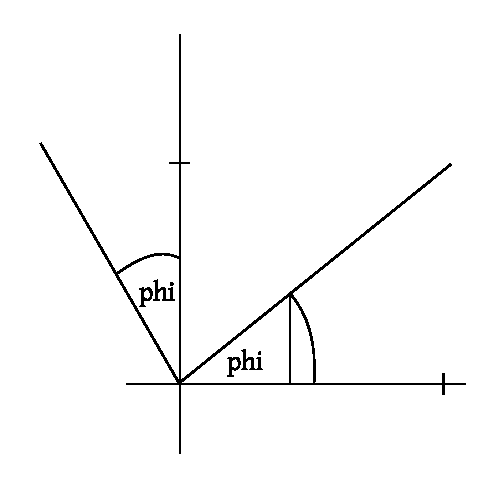
\includegraphics{img/rotation_in_R2.pdf}
    \caption{Rotation in $\mathbb R^2$}
  \end{center}
\end{figure}

\begin{rem}
  Newton considered motion (compare with Figure~\ref{img:motion}). We derive componentwise.
  \begin{figure}[!h]
    \begin{center}
      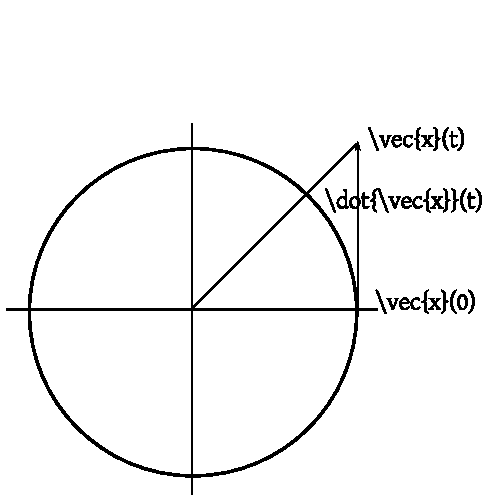
\includegraphics{img/motion.pdf}
      \caption{Motion}
      \label{img:motion}
    \end{center}
  \end{figure}
  \[ \hat{x}(t) = \begin{bmatrix} 0 & -1 \\ 1 & 0 \end{bmatrix} \cdot x(t) \]
  \[ \hat{x} = \alpha x \]
  \[ \frac{dx}{dt} = \alpha x \]
  \[ \frac{dx}{x} = \alpha dt \]
  \[ \int \frac{dx}{x} \int \alpha \, dt \]
  \[ \log(x) = \alpha t \Rightarrow x = e^{\alpha t} \cdot e^c + c \]
  \[ x(0) = e^c \]

  \[ \Rightarrow x(t) = e^{\begin{bmatrix} 0 & -1 \\ 1 & 1 \end{bmatrix} t} \cdot x(0) \]
  \[
    e^x = \sum_{n=0}^\infty \frac{x^n}{n!}
        = \sum_{n=0}^\infty \frac{\begin{bmatrix} 0 & -1 \\ 1 & 0 \end{bmatrix}^n}{n!} t^n
  \]

  \[ \begin{bmatrix} 0 & -1 \\ 1 & 0 \end{bmatrix}^2 = \begin{bmatrix} -1 & 0 \\ 0 & -1 \end{bmatrix} \]
  \[ \begin{bmatrix} 0 & -1 \\ 1 & 0 \end{bmatrix}^3 = \begin{bmatrix} 0 & 1 \\ -1 & 0 \end{bmatrix} \]
  \[ \begin{bmatrix} 0 & -1 \\ 1 & 0 \end{bmatrix}^4 = I \]
  This holds for any $M^{4i}, M^{4i+1}, M^{4i+2}$ and $M^{4i+3}$ respectively.

  \[ e^{i\varphi} = \sum_{n=0}^\infty \frac{(i\varphi)^n}{n!} = \sum_{n=0}^\infty \frac{(-1)^n \varphi^{2n}}{2n!} + \sum_{n=0}^{\infty} (-1)^n i \frac{\varphi^{2n+1}}{2(n+1)!} = \cos{\varphi} + i \sin{\varphi} \]
  \[ e^{\begin{bmatrix} 0 & -1 \\ 1 & 0 \end{bmatrix} \varphi} = I \cos{\varphi} + \begin{bmatrix} 0 & -1 \\ 1 & 0 \end{bmatrix} \sin{\varphi} = \begin{bmatrix} \cos{\varphi} & -\sin{\varphi} \\ \sin{\varphi} & \cos{\varphi} \end{bmatrix} \]
\end{rem}
\begin{rem}
  \fbox{Sophus Lie}

  Unitary matrices build a group. This defines the field of Lie groups.
\end{rem}

\begin{figure}[!h]
  \begin{center}
    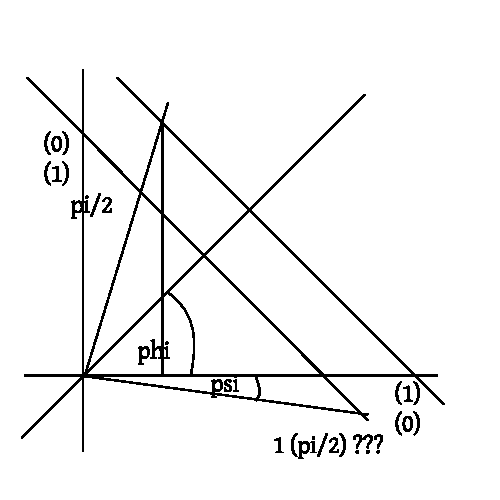
\includegraphics{img/reflection_in_r2.pdf}
    \caption{Reflection in R2}
    \label{img:refl-r2}
  \end{center}
\end{figure}

\begin{rem}[Reflection]
  \[
    U = \begin{bmatrix}
      \cos{2\varphi} & \cos(2\varphi - \frac\pi2) \\
      \sin{2\varphi} & \sin(2\varphi - \frac\pi2)
    \end{bmatrix} = \begin{bmatrix}
      \cos{2\varphi} & \sin{2\varphi} \\
      \sin{2\varphi} & -\cos{2\varphi}
    \end{bmatrix}
  \]
\end{rem}

\begin{theorem}
  \label{satz-8.73}
  The following sets are groups:
  \[ \mathcal O(n) = \setdef{U \in \mathbb R^{n \times n}}{U^t U = I} \qquad \text{ orthogonal group} \]
  \[ \mathcal U(n) = \setdef{U \in \mathbb U^{n \times n}}{U^t U = I} \qquad \text{ unitary group} \]
  \[ S\mathcal O(n) = \setdef{U \in \mathcal O(n)}{\det{U} = 1} \qquad \text{ special orthogonal group} \]
  \[ S\mathcal U(n) = \setdef{U \in \mathcal U(n)}{\det{U} = 1} \qquad \text{ special unitary group} \]
  \enquote{Classical} Lie groups.
\end{theorem}

\begin{theorem}
  For $U \in \mathcal U(n)$ it holds that $\abs{\det{U}} = 1$.
  \[ U^* = U^{-1} \]

  \begin{align*}
    \det{U^*} & =\det{\overline{U^t}} \\
      &= \overline{\det{U^t}} \\
      &= \overline{\det{U}} \\
      &= \det{U^{-1}} \\
      &= \frac{1}{\det{U}} \\
      &\Rightarrow \overline{\det{U}} \cdot \det{U} = 1
  \end{align*}
\end{theorem}

\begin{rem}
  \[ \mathcal O(n) = \set{\det(U) = 1} \cup \set{\det(U) = -1} \]
\end{rem}

\begin{ex}[$\mathcal O(2)$]
  Rotation:
  \[ \begin{bmatrix} \cos(\varphi) & -\sin(\varphi) \\ \sin{\varphi} & \cos{\varphi} \end{bmatrix} \qquad \det = 1 \]
  Reflection:
  \[ \begin{bmatrix} \cos(2\varphi) & \sin(2\varphi) \\ \sin{2\varphi} & -\cos{2\varphi} \end{bmatrix} \qquad \det = -1 \]
  Orthogonal:
  \[ U = \begin{bmatrix} a & b \\ c & d \end{bmatrix} \]
  \[
    \begin{cases}
      a^2 + c^2 &= 1 \\
      b^2 + d^2 &= 1 \\
      ab + cd   &= 0
    \end{cases}
  \]
  \[ U = \begin{bmatrix} a & b \\ c & d \end{bmatrix} = \begin{bmatrix} \cos{\varphi} & \cos{\varphi} \\ \sin{\varphi} & \sin{\varphi} \end{bmatrix} \]
  \[ \cos(\varphi - \psi) = \cos{\varphi} \cos{\psi} + \sin{\varphi} \sin{\psi} = 0 \]
  \[ \psi = \varphi + (k + \frac12) \pi \]

  This sum equation can be derived from Euler:
  \[ e^{i (\alpha + i \beta)} = e^{i\alpha} e^{i\beta} \]
  \[ \cos(\alpha + \beta) + i \sin(\alpha + \beta) = (\cos{\alpha} + i \sin{\alpha})(\cos{\beta} + i \sin{\beta}) \]
  \[ = \cos{\alpha} \cos{\beta} - \sin{\alpha} \sin{\beta} + i (\sin{\alpha} \cos{\beta} + \cos{\alpha} \sin{\beta}) \]

  \begin{align*}
    \cos{\psi} &= \cos(\varphi + (k + \frac12) \pi) \\
      &= \cos{\varphi} \underbrace{\cos(k + \frac12)}_{=0} \pi - \sin{\varphi} \underbrace{\sin(k + \frac12)}_{\varepsilon \coloneqq \pm 1} \pi \\
      &= -\varepsilon \sin{\varphi} \\
    \sin{\psi} &= \sin(\varphi + (k + \frac12) \pi) \\
      &= \sin{\varphi} \underbrace{\cos(k + \frac12)}_{=0} \pi + \cos\varphi \sin(k + \frac12) \pi = \varepsilon \cos{\varphi}
  \end{align*}
\end{ex}

\begin{rem}
  \[
    U = \begin{bmatrix}
      \cos\varphi & -\sin\varphi \cdot \varepsilon \\
      \sin\varphi & \cos\varphi \cdot \varepsilon
    \end{bmatrix}
    =
    \begin{bmatrix}
      \cos{\varphi} & -\sin{\varphi} \\
      \sin{\varphi} & \cos{\varphi}
    \end{bmatrix} \cdot \begin{bmatrix}
      1 & 0 \\
      0 & \varepsilon
    \end{bmatrix}
  \]
  \[ \det{U} = \varepsilon \]

  $U$ is either a rotation (if $\det{U} = 1$) or rotation with reflection (if $\det{U} = -1$).
\end{rem}

\begin{rem}
  \[ S\mathcal O(2) = \text{ rotations } \cong \mathcal T = \setdef{e^{i\varphi}}{\varphi \in [0,2\pi[} \]
  \[ e^{i\varphi} e^{i\psi} = e^{i(\varphi + \psi)} \]
\end{rem}

\begin{rem}
  \fbox{William R. Hamilton (1805--1865)}
  \[ S\mathcal U(2) = \setdef{q \in H}{\norm{q} = 1} \]
  Defined the Hamilton operator. Extension to $\mathbb R$ (\enquote{quaternions}):
  \[ H = \setdef{a_0 + a_1 i + a_2 j + a_3 k}{a_0, a_1, a_2, a_3 \in \mathbb R} \]
  \[ i^2 = j^2 = k^2 = -1 \]
  \[ ij = k \qquad jk = i \qquad ki = j \]
  \[ ji = -1 \qquad kj = -i \qquad ik = -j \]
  Almost a field (inverse elements, but not commutative). A skew field.

  Octonionen (inverse elements, but not associative).
\end{rem}

\section{Polynomials and Algebras}
\index[English]{$\mathbb K$-Algebra}
\index[German]{\foreignlanguage{ngerman}{$\mathbb K$-Algebra}}
\begin{defi}
  $\mathbb K$ is a field.
  A $\mathbb K$-Algebra is a vector space $\mathcal A$ over $\mathbb K$
  with multiplication: $*: \mathcal A \times \mathcal A \to \mathcal A$
  such that
  \begin{enumerate}
    \item $u * (b + c) = u * b + u * c$
    \item $(a + b) * c = a * c + b * c$
    \item $\lambda \cdot (a * b) = (\lambda \cdot a) * b = a * (\lambda \cdot b)$
  \end{enumerate}
  where $\lambda$ is an algebra.
\end{defi}

\index[English]{Associative algebra}
\index[German]{\foreignlanguage{ngerman}{Assoziative Algebra}}
\index[English]{Commutative Algebra}
\index[German]{\foreignlanguage{ngerman}{Kommutative Algebra}}
\begin{rem}
  \label{bem-8.2}
  If it furthermore holds that
  \[ a * (b * c) = (a * b) * c \]
  then $\mathcal A$ is associative.

  If it furthermore holds that
  \[ a * b = b * a \]
  then $\mathcal A$ is called commutative.
\end{rem}

\index[English]{Convolution}
\index[German]{\foreignlanguage{ngerman}{Faltung}}
\index[German]{\foreignlanguage{ngerman}{Konvolution}}
\index[English]{Schur product}
\index[German]{\foreignlanguage{ngerman}{Schur Produkt}}
\index[English]{Hadamond product}
\index[German]{\foreignlanguage{ngerman}{Hadamond Produkt}}
\index[English]{Jacobi identity}
\index[German]{\foreignlanguage{ngerman}{Jakobi Identität}}
\index[English]{Commutator product}
\index[German]{\foreignlanguage{ngerman}{Kommutator Produkt}}
\begin{ex}
  \label{bsp-9.3}
  \begin{itemize}
    \item $(\mathbb K, +, * = \cdot)$ associative, commutative
    \item $\Hom(V, V) = \End(V)$
      \[ f * g \coloneqq f \circ g \]
      non-commutative, associative algebra.

      This is isomorphic to $(\mathbb K^{n\times n}, +, \cdot)$
      where $\cdot$ is matrix multiplication.

      \emph{Hadamond}- or \emph{Schur product}:
      \[ [a_{ij}] [b_{ij}] = [a_{ij}, b_{ij}] \]
    \item
      \[ \mathcal C[0,1] \]
      \[ (f * g)(t) = f(t) \cdot g(t) \]
      \emph{Convolution}:
      \[ (f * g)(t) = \int_0^1 f(t - s) g(s) \, ds \]
    \item
      Consider $(\mathbb R^3, +, \times)$ with cross product. $a\times b = -b \times a$.
      \[ (a \times b) \times c \neq a \times (b \times c) \]
      Non-associative, non-commutative.
    \item
      Consider $(\mathbb K^{n\times n}, +, [])$.
      \[ [A, B] = A \cdot B - B \cdot A \]
      Lie product or commutator product.
      Non-commutative, non-associative.
      From this, the \emph{Jacobi identity} follows.
    \item
      \[ = A = \mathbb K_{\text{symm}}^{n\times n} = \setdef{A}{A = A^t} \]
      \[ A * B = \frac{AB + BA}{2} \]
      Jordan product, associative, commutative.
  \end{itemize}
\end{ex}

\begin{defi}
  \label{defi-9.4}
  \[ \mathbb K^\infty = \setdef{(a_0, a_1, a_2, \ldots)}{a_i \in \mathbb K} \]
  Vector of all sequences.
  \[ P_{\mathbb K} = \setdef{(a_0, a_1, \ldots, a_n, 0, 0, \ldots)}{a_i \in \mathbb K, n \in \mathbb N} \]
  Subspace of finite sequences. Basis of $P_{\mathbb K}: (e_i)_{i \geq 0}$.

  \[ (a_n) * (b_n) = (c_n) \]
  \[ (c_n) = \sum_{k=0}^n a_k b_{n-k} \qquad \text{(Cauchy product)} \]
\end{defi}

\begin{theorem}
  \label{satz-9.5}
  \begin{enumerate}
    \item
      $(P_{\mathbb K}, *)$ is an associative, commutative $\mathbb K$-Algebra with one element
      $(1, 0, 0, \ldots) = e_0$. $P_{\mathbb K} = \mathbb K[x]$.

      \[ x^k \coloneqq e_k \]
      \[ e_i * e_j = e_{i+j} \]
      \[ x^0 = 1 \qquad \text{the one element} \]
    \item
      \[ \underbrace{\mathbb K[[x]]}_{\mathbb K(x)} = \setdef{\sum_{k=0}^\infty a_k x^k}{a_k \in \mathbb K} \]
      is a formal power series. Defines a commutative, associative algebra.
  \end{enumerate}
\end{theorem}

\meta{lecture}{4th of May 2016}{Franz Lehner}

\begin{rem}
  What is $\log(-1)$?
  \[ e^{i\varphi}= \cos{\varphi} + i \cdot \sin{\varphi} \]
  \[ e^{\log{-1}} = -1 \]
  \[ \Rightarrow e^{i\pi} = -1 \]
  \[ \Rightarrow \log(-1) = i\pi \]
  This is ambiguous.
  \[ \sqrt{-1} = \pm i \]
  \[ \sqrt[3]{i} = 1, e^{2\frac\pi i}{3}, e^{-2\frac{\pi i}{3}} \]
  \[ \sqrt{e^{ix}} = e^{\frac{ix}{2}} \]

  Riemann replaced the complex plane with a plane which consists of two planes.
  If you follow the unit circle one rotation, you end up at the other plane.
\end{rem}

\begin{rem}
  Consider $(P_{\mathbb K}, *)$.
  \[ P_{\mathbb K} = \setdef{(a_0, a_1, \ldots, a_n, 0, \ldots)}{a_k \in \mathbb K, n \in \mathbb N_0} \]
  with $(a_i) * (b_j) = (c_k)$ is an associative and commutative $\mathbb K$-algebra.
  \[ c_k = \sum_{j=i}^k a_j b_{k-j} = \sum_{j=0}^k a_{k-j} b_j \]
  \[ e_i * e_j = e_{i+j} \]
  \[ x^i \coloneqq e_i \]

  Let $a_i = 0$ for $i > m$, $b_j = 0$ for $j > n$.
  Compare with Figure~\ref{img:inf-abi}.
  \[ c_k = \sum_{i=0}^k a_i b_{k-i} = \sum_{i=0}^m a_i \underbrace{b_{k-i}}_{=0} = 0 \]
  \[ k > m + n  \qquad i < m \]
  \[ k - i > m + n - i \]
  \[ k - i > n \]

  \begin{figure}[!h]
    \begin{center}
      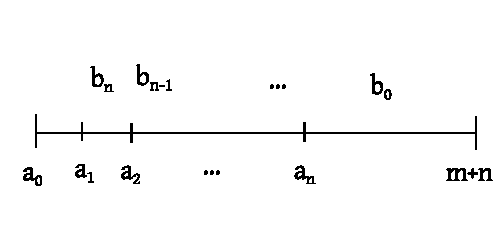
\includegraphics{img/polynomial_k-algebra.pdf}
      \caption{relation of $a_i$ and $b_i$}
      \label{img:inf-abi}
    \end{center}
  \end{figure}

  \[ \deg(p(x) \cdot q(x)) \leq \deg(p(x)) + \deg(q(x)) \]
  \[ p(x) = a_0 + a_1 x + \ldots + a_m x^m \]
  \[ \deg(p(x)) = \max\setdef{i}{a_i \neq 0} \]
  Distributive law:
  \[ (a * (b + c))_k = \sum_{i=0}^k a_i (b_{k-i} + c_{k-i}) = \sum_{i=0}^k a_i b_{k-i} + \sum_{i=0}^k a_i c_{k-i} = (a * b)_k + (a * c)_k \]

  This also works for $(a_0, a_1, \ldots)$ arbitrary sequences.
  $(a * b)_k = \sum_{i=0}^k a_i b_{k-i}$ is finite for all $k$.
  Polynomials (= finite sequences) form a subalgebra.
\end{rem}

\begin{defi}
  \label{defi-9.6}
  \[ X^0 = (1, 0, \ldots, 0) = 1 \]
  \[ X^k = (0, \ldots, 0, 1, 0, \ldots) \]
  \[ X^k \cdot X^l = X^{k+l} \]
  We write $\mathbb K[x]$ instead of $P_{\mathbb K}$.
  \[ p(x) = \sum_{i=0}^m a_i x^i \]
  \[ \partial p(x) = \deg(p(x)) = \max\setdef{i}{a_i \neq 0} \]
  We need to define $\deg(0) = -\infty$.
\end{defi}

\begin{lemma}
  \begin{enumerate}
    \item $\deg(p(x) \cdot q(x)) = \deg(p(x)) + \deg(q(x))$
    \item $\mathbb K[x]$ is zero divisor free.
      \[ p(x) q(x) = 0 \Rightarrow p(x) = 0 \lor q(x) = 0 \]
      Counterexamples for zero divisor freedom:
      \[ \mathbb Z_n, n \not\in \mathbb P: n = pq \Rightarrow p \neq 0 \mod{n} \land q \neq 0 \mod{n} \]
      \[ \begin{bmatrix} 1 & 0 \\ 0 & 0 \end{bmatrix} \cdot \begin{bmatrix} 0 & 0 \\ 0 & 1 \end{bmatrix} = 0 \]
  \end{enumerate}
\end{lemma}

\begin{defi}
  \label{defi-9.8}
  Every polynomial $p(x) \in \mathbb K[x]$ induces a function.
  \[ p: \mathbb K \to \mathbb K \]
  \[ \alpha \mapsto p(\alpha) = \sum_{k=0}^m a_k \alpha^k \]

  \[ (\lambda p + \mu q)(\alpha) = \lambda p(\alpha) + \mu q(\alpha) \]
  \[ (p \cdot q)(\alpha) = p(\alpha) \cdot q(\alpha) \]

  \[ \mathbb K[x] \to \mathbb K^{\mathbb K} \]
  is an algebra homomorphism.
\end{defi}
\begin{rem}
  Is it injective?
  If $\abs{\mathbb K} < \infty$, it is not injective.
  \[ \dim{\mathbb K[x]} = \infty \qquad \dim{{\mathbb K}^{\mathbb K}} = \abs{\mathbb K} \]
  \[ p(x) = (x - \xi_1)(x - \xi_2) \ldots (x - \xi_n) \]
  has degree $n$.

  From this we can see the difference between a polynomial and a polynomial function.
\end{rem}

\begin{ex}
  Every function $f: \mathbb K \to \mathbb K$ is a polynomial function,
  hence there exists some polynomial $p(x) \in \mathbb K[x]$ such that $p(\xi) = f(\xi)$ for all $\xi \in \mathbb K$.
\end{ex}

\index[English]{Algebra homomorphism}
\index[German]{\foreignlanguage{ngerman}{Algebra Homomorphismus}}
\begin{defi}
  \label{defi-9.10}
  A map $\psi: \mathcal A \to \mathcal B$ between two $\mathbb K$-algebras $\mathcal A$ and $\mathcal B$
  is called \emph{algebra homomorphism} if $\Psi$ is linear and multiplicative.
  \[ \bigwedge_{a,b \in \mathcal A} \psi(a *_{\mathcal A} b) = \psi(a) *_{\mathcal B} \psi(b) \]
\end{defi}

\begin{ex}
  \label{ex-9.11}
  \begin{itemize}
    \item $\mathbb K[x] \to {\mathbb K}^{\mathbb K}$ with $p(x) \mapsto$ polynomial function
    \item For all $\alpha \in \mathbb K$,
      \[ \psi_\alpha: \mathbb K[x] \to \mathbb K \]
      \[ p(x) \mapsto p(\alpha) \]
      is algebra homomorphism.
    \item $\mathbb K \to \mathbb K[x]$ with $\alpha \to \alpha \cdot \mathbb 1$.
      Embedding is algebra homomorphism.
  \end{itemize}
\end{ex}

\begin{theorem}[Insertion theorem] % TODO: dt. Einsetzungssatz - correct translation?
  \label{theorem-9.12}
  Let $\mathcal A$ be an associative algebra over $\mathbb K$ with one-element
  $1_{\mathcal A}$.
  \begin{itemize}
    \item
      \[ \Rightarrow: L: \mathbb K \to \mathcal A \]
      \[ \alpha \mapsto \alpha \cdot {\mathbb A_{\mathcal A}} \]
      is an algebra homomorphism.
    \item For every $a \in \mathcal A$ is a map
      \[ \psi_a: \mathbb K[x] \to \mathcal A \]
      \[ \sum_{k=0}^n c_k x^k \mapsto \sum_{k=0}^n c_k a^k \]
      where $a^0 \coloneqq 1_{\mathcal A}$ and $a^{k+1} = a * a^k$,
      the \emph{unique} algebra homomorphism $\psi: \mathbb K[x] \to \mathcal A$
      with the property $\psi(x) = a$.

    \item
      Every algebra homomorphism $\psi: \mathbb K[x] \to \mathcal A$ has this structure.
  \end{itemize}
\end{theorem}
\begin{proof}
  If $a = \psi(x)$, then $a^k = \psi(x)^k = \psi(x^k)$.
  If $\psi(x)$ is known, then $\psi(x^k)$ is defined for all $k$.
  So $\psi(p(x))$ is defined for all $p(x) \in \mathbb K[x]$.
  This follows because they represent a basis and by the Fortsetzungssatz. % TODO: translation
\end{proof}

\begin{rem}
  Linearity of $\psi_{a}$ will be shown in the practicals.
  Multiplicativity:
  \[ \psi_a(p(x) \cdot q(x)) \stackrel!= \psi_a(p(x)) * \psi_a(q(x)) \]
  Let $p(x) = \sum_{i=0}^m \alpha_i \cdot x^i$ and $q(x) = \sum_{j=0}^n \beta_j x^j$.
  \[ p(x) \cdot q(x) = \sum_{k=0}^{m+n} \gamma_k x^k \qquad \gamma_k = \sum_{i=0}^k \alpha_i \beta_{k-i} \]
  \[ \psi_a(p(x) \cdot q(x)) = \sum_{k=0}^{m+n} \gamma_k a^k \]
  \begin{align*}
    \psi_a(p(x)) * \psi_a(q(x)) &= \left(\sum_{i=0}^m \alpha_i a^i\right) \cdot \left(\sum_{j=0}^n \beta_j a^j\right) \\
        &= \sum_{i=0}^m \sum_{j=0}^n \alpha_i \beta_j a^{i+j} \\
        &= \sum_{k=0}^{m+n} \underbrace{\sum_{i,j \geq 0} \alpha_i \beta_j}_{\sum_{i=0}^k \alpha_i \beta_{k-i} = \gamma_k} a^k \\
  \end{align*}
\end{rem}

\begin{rem}[Notation]
  \[ \psi_a(p(x)) \eqqcolon p(a) \]
\end{rem}

\begin{ex}
  \label{ex-9.13}
  \begin{itemize}
    \item $\mathcal A = \mathbb K$
      \[ \psi_{\alpha}(p(x)) = p(\alpha) \]
    \item $\mathcal A = \Hom(V,V)$
      \[ L: \mathbb K \to \Hom(V,V) \]
      \[ \lambda \mapsto \lambda \cdot \operatorname{id} \]

      \[ f^0 = \operatorname{id} \]
      \[ f^k = \underbrace{f \circ f \circ \ldots \circ f}_{kx} \Rightarrow \psi_f\left(\sum_{k=0}^n \alpha_k x^k\right) = \sum_{k=0}^n \alpha_k f^k \]
    \item $\mathcal A = \mathbb K^{n\times n}$
      \[ \psi_A(p(x)) = p(A) = \sum_{k=0}^n \alpha_k A^k \]
  \end{itemize}
\end{ex}

\begin{rem}
  $\mathbb K[x]$ is a free associative algebra with a generator over $\mathcal A$.
  Every map $f: \set{X} \to \mathcal A$ has a unique continuous to an algebra homomorphism.
  \[ \psi: \mathbb K[x] \to \mathcal A \]
  $\mathbb K[x]$ is the smallest algebra over $\mathbb K$ which contains $x$.

  For two generators?
  \[
    \begin{array}{ccc}
      f: \set{x,y}                    & \to & \mathcal A \\
      \downarrow                      &       & \\
      \psi: \mathbb K\functional{x,y} & \to & \mathcal A
    \end{array}
  \]
  is a non-commutative polynomial in $x,y$.

  Analogously: free group, free monoid and every vector space is free over its basis.
\end{rem}

\index[English]{Roots of functions}
\index[German]{\foreignlanguage{ngerman}{Nullstellen von Funktionen}}
\begin{defi}
  \label{defi-9.15}
  Let $p(x) \in \mathbb K[x]$.
  A root of $p(x)$ is some $\xi \in \mathbb K$ such that $p(\xi) = 0$.
  \[ \Leftrightarrow p(x) \in \kernel(\psi_\xi) \]
\end{defi}

\begin{ex}
  \[ p(x) = a_0 \]
  No non-trivial roots.
  \[ p(x) = a_0 + a_1 x + a_2 x^2 \]
  The solution equation was found 2000~BC.
  \[ p(x) = a_0 + a_1 x + a_2 x^2 + a_3 x^3 \]
  Equation of Cardano.

  \fbox{Gerdama Cardano (1501--1576)} \\
  \enquote{Ars Magna} (1545)

  \fbox{Niccolo Tartaglia (1499-1557)}

  Niccolo Tartaglia found the solution to Cardano's equation.
  But actually \fbox{Siphione del Forzzo (1465--1526)} found the equation first
  and forwarded it to his student Antonio Fiore.
  This was also the first time someone reasoned about complex numbers.
  They did not get explicitly defined.

  $\deg(p(x)) = 4$ (L. Ferrari)

  $\deg(p(x)) \geq 5$ (1826, Abel)
\end{ex}

\begin{rem}[Cadano and Tartaglia formula]
  \label{bem-9.16}
  Originally: cub pi6 reb e$\overline{\textrm{q}}$lis 20
  \[ x^3 + 6x = 20 \]

  Approach: $x = u + v$.

  \[ (u + v)^3 + 6 (u + v) = 20 \]
  \[ u^3 + 3u^2 v + 3uv^2 + v^3 + 6 (u + v) = 20 \]
  \[ = u^3 + v^3 + (3uv + 6) (u + v) = 20 \]

  We choose $v$ such that $3uv + 6 = 0$.
  \[ \Rightarrow uv = -2 \]
  \[ \Rightarrow u^3 v^3 = -18 \]
  \[ u^3 + v^3 = 20 \]

  Let $a = u^3$ and $b = v^3$.
  \[ a \cdot b = -8 \land a + b = 20 \Rightarrow a(20 - a) = -8 \]
  \[ a^2 - 20a - 8 = 0 \]
  \[ a = \frac{20 \pm \sqrt{400 + 32}}{2} = 10 \pm \sqrt{108} \]
  \[ \Rightarrow u^3 = 10 + \sqrt{108} \]
  \[ v^3 = 10 - \sqrt{108} \]
  \[ x = u + v = \sqrt[3]{10 + \sqrt{108}} + \sqrt[3]{10 - \sqrt{108}} \]
\end{rem}

\begin{theorem}[Division with remainder]
  \label{satz-9.17}
  Let $p(x), q(x) \in \mathbb K[x]$ and $q(x) \neq 0$.
  Then there exists exactly one $s(x), r(x) \in \mathbb K[x]$ such that $\deg(r(x)) < \deg(q(x))$
  and $p(x) = s(x) \cdot q(x) + r(x)$.

  Compare this with natural numbers and the extended euclidean algorithm.
  \[ m \in \mathbb Z, n \in \mathbb N \Rightarrow \exists! a,b: m = a\cdot n + b \text{ with } 0 \leq b < n \]
\end{theorem}

\begin{proof}
  Complete induction over $\deg(p(x))$.
  \begin{description}
    \item[Case 1: $\deg(p(x)) < \deg(q(x))$]
      \[ \Rightarrow p(x) = 0 \cdot q(x) + p(x) \]
      is unique.
    \item[Case 2: $\deg(p(x)) \geq \deg(q(x))$]
      \[ p(x) = \sum_{k=0}^m a_k x^k \qquad q(x) = \sum_{l=0}^n b_l x^l \]
      $m \geq n$.
      Let $p_1(x) = p(x) - \frac{a_m}{b_n} x^{m-n} \cdot q(x)$.
      \begin{align*}
        &= \sum_{k=0}^m a_k x^k - \sum_{l=0}^n \frac{a_m}{b_n} b_l x^{m-n+l} \\
        &= \sum_{k=0}^{m-1} a_k x^k - \sum_{l=0}^{n-1} \frac{a_m}{b_n} b_l x^{m-n+l}
      \end{align*}
      $\deg(p_1(x)) < \deg(p_2(x))$.

      Induction hypothesis $\Rightarrow p_1(x) = s_1(x) \cdot q(x) + r_1(x)$
      \[ \Rightarrow p(x) = \left(\frac{a_m}{b_n} x^{m-n} + s_1(x)\right) q(x) + r_1(x) \]
      \[ = p_1(x) + \frac{a_m}{b_n} x^{m-n} \cdot q(x) \]
  \end{description}
\end{proof}

% TODO: reformat
\begin{ex}
  \label{bsp-9.18}
  \[
    \begin{array}{rl}
      3x^5 - x^4 + 2x^3 + x^2 + 1 &: x^2 - 3x + 1 = 3x^3 + 8x^2 + 23x + 62 \\
      -(3x^5 - 9x^4 + 3x^3)       &\\
    \hline
      0 + 8x^4 - x^3 + x^2 + 1 \\
      0 - (8x^4 - 24x^3 + 8x^2) \\
    \hline
      0 + 0 + 23x^3 - 7x^2 + 1 \\
      0 + 0 - 23x^3 - 69x^2 + 23x \\
    \hline
      0 + 0 + 62x^2 - 23x + 1 \\
      0 + 0 + 62x^2 - 186x + 62 \\
    \hline
      0 + 0 + 0 + 163x - 61 = r(x)
    \end{array}
  \]
\end{ex}

\meta{lecture}{9th of May 2016}{Franz Lehner}
\begin{rem}
  An Euclidean ring is a ring in which the extended Euclidean algorithm works.
\end{rem}
\begin{theorem}
  Let $p(x), q(x) \in \mathbb K[x]$ and $q(x) \neq 0$.
  Then there exists exactly one $s(x)$ and $r(x)$ such that $\deg{r(x)} < \deg{q(x)}$.
  \[ p(x) = r(x) \cdot q(x) + r(x) \]
\end{theorem}

\index[English]{Division of a polynomial by a polynomial}
\index[German]{Division eines Polynoms durch einen Polynom}
\begin{defi}
  \label{defi-9.19}
  $q(x)$ divides $p(x)$ if $\exists s(x): p(x) = s(x) \cdot q(x)$
  (i.e. division happens without remainder).
\end{defi}

\begin{theorem}
  \label{defi-9.20}
  Consider $q(x) = x - \xi$.
  \[ \Rightarrow p(x) = s(x) \cdot (x - \xi) + r \]
  \[ \Rightarrow p(\xi) = r \]
\end{theorem}

\begin{cor}
  $\xi$ is a root of $p(x)$ $\Leftrightarrow x - \xi$ is divisor of $p(x)$.
\end{cor}

\begin{theorem}[Horner schema]
  Let $p(x) \in \mathbb K[x]$ and $\lambda \in \mathbb K$.
  Determine $p(\lambda)$.

  \[ p(x) = a_n x^n + a_{n-1} x^{n-1} + \ldots + a_{1} x + a_0 \]
  \[ p(\lambda) = a_n \lambda^n + a_{n-1} \lambda^{n-1} + \ldots + a_{1} \lambda + a_0 \]
\end{theorem}

\begin{rem}
  Naively it requires a quadratic number of evaluations (for $\lambda$, per $\lambda-1$, per \dots = $\frac{n(n+1)}{2} \approx n^2$).
  Using binary composition it takes a logarithmic times linear number of evaluations (for $\lambda$, for $\lambda-1$, \dots).
  However, it also works with $n$ multiplications.
  \[ p(x) = (a_n \lambda^{n-1} + a_{n-1} \lambda^{n-2} + \ldots + a_1) \lambda + a_0 \]
  \[ = ((a_n \lambda^{n-2} + a_{n-1} \lambda^{n-3} + \ldots + a_2)\lambda + a_1) \lambda + a_0 \]
\end{rem}

\begin{ex}
  \begin{align*}
    p(x) &= a_3 \lambda^3 + a_2 \lambda^2 + a_1 \lambda + a_0  & a_3 \\
         & (a_3 \lambda^2 + a_2 \lambda + a_1) \lambda + a_0   & a_3 \lambda + a_2 \\
         & ((a_3 \lambda + a_2) \lambda + a_1) \lambda + a_0   & ((a_3 \lambda + a_2) \lambda + a_1) \lambda + a_0
  \end{align*}

  Algorithm:
  \[ \xi_n = a_n \text{ for } k = n-1, \ldots, 0 \]
  \[ \xi_k = \lambda \xi_{k+1} + a_k \]
  \[ \Rightarrow p(\lambda) = \xi_0 \]

  We evaluate:
  \[ p(x) = 3x^5 - x^4 + 2x^3 + x^2 + 1 \]
  Let $\lambda = 5$.
  \begin{align*}
    \xi_5 &= 3 \\
    \xi_4 &= 5 \cdot 3 -1 = 14 \\
    \xi_3 &= 5 \cdot 14 + 2 = 72 \\
    \xi_2 &= 5 \cdot 72 + 1 = 361 \\
    \xi_1 &= 5 \cdot 36 + 0 = 1805 \\
    \xi_0 &= 5 \cdot 1805 + 1 = 9026 \\
  \end{align*}
  Compare with division:
  % TODO: reformat
  \[
    \begin{array}{rl}
      3x^5 - x^4 + 2x^3 + x^2 + 1 &: x - 5 = 3x^4 + 14x^3 + 72x^2 + 361x + 1805 \\
      3x^5 - 15x^4 \\
    \hline
      0 + 14x^4 + 2x^3 + x^2 + 1 \\
      0 + 14x^4 - 70x^3 \\
    \hline
      0 + 0     + 72x^3 + x^2 + 1 \\
      0 + 0     + 72x^3 - 360x^2 \\
    \hline
      0 + 0     + 0     + 361x^2 + 1 \\
      0 + 0     + 0     + 361x^2 - 1805x \\
    \hline
      0 + 0     + 0     + 0      + 1805x + 1 \\
      0 + 0     + 0     + 0      + 1805x - 5 \cdot 1805 \\
    \hline
      0 + 0     + 0     + 0      + 0     + 9026
    \end{array}
  \]

  The Horner scheme is equivalent to division, but written down more efficiently.
\end{ex}

\index[English]{Irreducible polynomial}
\index[German]{\foreignlanguage{ngerman}{Irreduzibler Polynom}}
\begin{defi}
  \label{defi-9.23}
  A polynomial $p(x) \in \mathbb K[x]$ is called \emph{reducible}
  if $\exists p_1(x) \exists p_2(x) \in \mathbb K[x]: \deg{p_1(x)}, \deg{p_2(x)} < \deg{p(x)}$
  and $p(x) = p_1(x) \cdot p_2(x)$ (hence there exists a non-trivial divisor). % TODO: echter Teiler == non-trivial divisor?!
  Otherwise $p(x)$ is called irreducible.
\end{defi}

\begin{rem}
  \label{bem-9.24}
  \begin{itemize}
    \item Constant and linear polynomials are irreducible.
    \item Irreducible polynomials of degree $\geq 2$ have no roots
      (otherwise $x - \xi$ is divisor!)
  \end{itemize}
\end{rem}

\begin{ex} \hfill{}
  \begin{itemize}
    \item $x^2-2$ is irreducible in $\mathbb K = \mathbb Q$.
      Is reducible in $\mathbb K = \mathbb R$ with $(x - \sqrt{2})(x + \sqrt{2})$.
    \item $x^2 + 1$ is irreducible in $\mathbb K = \mathbb Q$ and $\mathbb K = \mathbb R$
      and reducible in $\mathbb K = \mathbb C$ with $(x - i)(x + i)$.
    \item $x^2 + x + 1 \in \mathbb Z_2[x] \Rightarrow$ irreducible.
      \[ x^3 + x + 1 \text{ is irreducible} \]
      \[ x^5 + x + 1 = (x^2 + x + 1)(x^3 + x^2 + 1) \text{ is reducible} \]
  \end{itemize}
\end{ex}

\begin{rem}
  How about explicitly defining fields such that $x^2 + x + 1$ is reducible?

  Consider $(\sqrt{-1})^2 + 1 = 0$.
  In which field does $x^2 + x + 1 \in \mathbb Z_2[x]$ have a root?

  Let $\alpha$ be a \enquote{number} such that $\alpha^2 + \alpha + 1 = 0$.
  \[ \Rightarrow \alpha^2 = \alpha + 1 \]
  \[ \alpha^3 = \alpha (\alpha + 1) = \alpha^2 + \alpha = \alpha + 1 + \alpha = 1 \]
  \begin{align*}
    (a \cdot \alpha + b) (c \cdot \alpha + d)
      &= ac \cdot \underbrace{\alpha^2}_{=\alpha + 1} (b \cdot c + a \cdot d) \cdot \alpha + bd \\
      &= (ac + bc + ad) \alpha + (ac + bd)
  \end{align*}
  \[ \Rightarrow \setdef{a \cdot \alpha + b}{a,b \in \mathbb Z_2} \eqqcolon \operatorname{GF}(2^2) = \operatorname{GF}(4) \]
  is a ring and even a field\footnote{GF stands for Galois field}.
  For the practicals you need to determine the inverse $\alpha^{-1} = \alpha^2$.

  For all $p \in \mathbb P$ (and $k \in \mathbb N$) you need to consider a different Galois field $\operatorname{GF}(p^k)$ (is a field of order $p^k$).
\end{rem}

\begin{theorem}{Fundamental theorem of algebra}
  $\mathbb C$ is algebraically closed,
  hence every polynomial $p(x) \in \mathbb C[x]$ has a root $\xi \in \mathbb C$.
  Corollaries:
  \begin{enumerate}
    \item $p(x) \in \mathbb C[x]$ is irreducible $\Leftrightarrow \deg{p(x)} \leq 1$
    \item Every $p(x) \in \mathbb C[x]$ has a factor ring
      \[ p(x) = (x - \xi_1) (x - \xi_2) \ldots (x - \xi_n) \]
      where $\xi_i \in \mathbb C$ and $n = \deg{p(x)}$.
  \end{enumerate}
\end{theorem}
\begin{proof}
  No proof given.

  This theorem cannot be proven with means of algebra.
  You need to study theory of complex functions.

  \[ f'(z_0) = \lim_{z \to z_0} \frac{f(z) - f(z_0)}{z - z_0} \]

  Theorem of Lionville: Every complex differentiable function is unbounded.
\end{proof}

\begin{theorem}
  \label{satz-9.27}
  In arbitrary fields it holds that:
  every polynomial has (except for the order) a unique factorization
  $p(x) = p_n(x) \ldots p_k(x)$ to irreducible factors.
\end{theorem}

\index[English]{Greatest common polynomial divisor}
\index[German]{\foreignlanguage{ngerman}{Größter gemeinsamer Polynomteiler}}
\begin{theorem}
  Let $p(x)$ and $q(x) \in \mathbb K[x] \setminus \set{0}$.
  Then there exists a unique monic polynomial (ie. leading coefficient $1$)
  of maximum degree denoted $\operatorname{gcd}(p(x), q(x))$
  such that
  \[ \divides{\operatorname{gcd}(p,q)}{p(x)} \land \divides{\operatorname{gcd}(p,q)}{q(x)} \]
  Then it holds that \emph{all} common divisors of $p(x)$ and $q(x)$
  divide $\operatorname{gcd}(p(x), q(x))$.
\end{theorem}

\begin{proof}
  Let $g(x)$ be a polynomial of maximum degree, which divides $p(x)$ and $q(x)$.
  \[ \Rightarrow p(x) = f(x) \cdot g(x) \qquad q(x) = h(x) \cdot g(x) \]
  Let $d(x)$ be a common divisor, then $\deg{d(x)} \leq \deg{g(x)}$.
  We apply division to retrieve $g(x) = s(x) \cdot d(x) + r(x)$
  and $\deg{r(x)} < \deg{d(x)}$.
  \[ p(x) = \tilde{f}(x) \cdot d(x), \qquad q(x) = \tilde{h}(x) \cdot d(x) \]

  It holds that
  \[ f(x) \cdot g(x) = \tilde{f}(x) \cdot d(x) \]
  \[ f(x) \cdot g(x) = f(x) \left(s(x) d(x) + r(x)\right) \]
  \[ \left(\tilde{f}(x) - f(x) \cdot s(x)\right) \cdot d(x) = r(x) \]
  \[ \deg{(\text{LHS})} > \deg{(\text{RHS})} \]
  \[
    \Rightarrow \tilde{f}(x) = f(x) \cdot s(x) = 0
    \Rightarrow r(x)= 0 \Rightarrow \divides{d(x)}{g(x)}
  \]
\end{proof}

\begin{rem}
  Only one unique greatest common divisor can exist.
  Proof is given in the practicals.

  If $p(x) = s(x) \cdot q(x) + r(x)$
  \[ \Rightarrow \operatorname{gcd}(p(x), q(x)) = \operatorname{gcd}(q(x), r(x)) \]
  just like for integers.
\end{rem}

\index[English]{Multiplicity}
\index[German]{\foreignlanguage{ngerman}{Vielfachheit}}
\begin{defi}
  A root $\xi$ of a polynomial $p(x)$ has multiplicity $m$
  if $\divides{(x - \xi)^{m}}{p(x)}$ but $(x - \xi)^{m+1} \,\not\mid\, p(x)$.
\end{defi}

\begin{rem}
  In the practicals we will see that the roots with multiplicity $\geq 2$
  are the roots of the greatest common divisor $p(x)$ and $q(x)$.
  \[ (x^n)' = nx^{n-1} \]
\end{rem}

\section{Eigenvalues and Eigenvectors}
%
\index[English]{Eigenvalues}
\index[German]{\foreignlanguage{ngerman}{Eigenwerte}}
\index[English]{Eigenvectors}
\index[German]{\foreignlanguage{ngerman}{Eigenvektoren}}
\index[English]{Equivalence transformation}
\index[German]{\foreignlanguage{ngerman}{Äquivalenztransformation}}
Our goal is to find $f \in \End(V) = \Hom(V, V)$ of a basis $B$ such that
$\Phi_B^B(f)$ has the simplest possible structure or find (for a given matrix $A$)
a matrix $T$ such that
\[ T A T^{-1} \]
has the simplest possible structure (\enquote{equivalence transformation}).

Compare it with
\[
  \Phi_C^B(f) =
    \begin{bmatrix}
      1 &        &   &   \\
        & \ddots &   &   \\
        &        & 1 &   \\
        &        &   & 0
    \end{bmatrix}
\] \[
  UAV = \begin{bmatrix}
    1 &        &   &   \\
      & \ddots &   &   \\
      &        & 1 &   \\
      &        &   & 0
  \end{bmatrix}
\]

\index[English]{Spectrum}
\index[German]{\foreignlanguage{ngerman}{Spektrum}}
\begin{defi}
  \label{defi-10.1}
  Let $V$ be a vector space over $\mathbb K$. Let $f \in \End{V}$.
  $\lambda \in \mathbb K$ is called eigen value of $f$
  if there exists $v \in V \setminus \set{0}: f(v) = \lambda \cdot v$.
  $v$ is called eigen vector of a vector value $\lambda$.

  \[ \spec(f) \coloneqq \setdef{\lambda}{\lambda \text{ is eigenvalue of } f} \]
  is called \emph{spectrum} of $f$.
\end{defi}

\index[English]{Eigenspace}
\index[German]{\foreignlanguage{ngerman}{Eigenraum}}
\begin{lemma}
  \label{lemma-10.2}
  \[ \eta_\lambda = \setdef{v \in V}{f(v) = \lambda v} = \kernel(\lambda \cdot \text{id} - f) \]
  is a subspace and is called Eigenspace of $f$ for eigenvalue $\lambda$.

  \[ v \in \eta_{\lambda} \Leftrightarrow f(v) = \lambda \cdot v \]
  \[ \Leftrightarrow \lambda \cdot v - f(v) = 0 \]
  \[ \Leftrightarrow (\lambda \cdot \text{id} - f)(v) = 0 \]
  \[ \Leftrightarrow v \in \kernel(\lambda \cdot \text{id} - f) \]
\end{lemma}

\begin{ex}
  \label{bsp-10.3}
  \begin{itemize}
    \item Let $f = c \cdot \text{id}$
      \[ \Rightarrow f(v) = c \cdot v \qquad \text{ for all } v \in V \]
      \[ \Rightarrow \spec(f) = \set{c} \]
      \[ \lambda = c \qquad \eta_\lambda = V \]
    \item
      Let $B$ be a basis of $V$
      \[ f: V \to V \]
      \[ b_i \mapsto \lambda_i \cdot b_i \]
      and continuation theorem: $f(\sum \alpha_i b_i) = \sum \alpha_i \lambda_i b_i$.
      \[
        \Leftrightarrow \Phi_B^B(f) = \begin{bmatrix}
          \lambda_1 &        & \\
                    & \ddots & \\
                    &        & \lambda_n
        \end{bmatrix}
      \]

      \[ \Rightarrow \spec(f) = \set{\lambda_1, \ldots, \lambda_n} \]
      \[ \eta_\lambda = \mathcal L\left(b_i \left| \lambda_i = \lambda\right)\right. \]
      Let $\lambda$ be an Eigenvalue.

      \[
        \Rightarrow \exists v = \sum \alpha_i b_i:
        f\left(\sum \alpha_i b_i\right) = \lambda \cdot \sum_{i=1}^n \alpha_i b_i
      \] \[
        \sum \alpha_i b_i = \sum_{i=1}^n \alpha_i \lambda_i b_i
      \] \[
        \sum (\lambda - \lambda_i) \alpha_i b_i = 0
      \] \[
        (b_i) \text{ is linear independent} \Rightarrow (\lambda - \lambda_i) \alpha_i = 0 \forall i
      \] \[
        \lambda = \lambda_i \lor \alpha_i = 0
      \]
    \item
      \[ V = C^{\infty}(\mathbb R) \]
      \[ \frac{d}{dx}: C^{\infty} \to C^{\infty} \]
      \[ f \mapsto f' = \frac{df}{dx} \]
      Eigenvectors?
      \[ y' = \lambda y \]
      \[ \frac{dy}{dx} = \lambda y \Rightarrow \frac{dy}{y} = \lambda dx \]
      \[ \int \frac{dy}{y} = \lambda \int dx \]
      \[ \log{y} = \lambda x + C \]
      \[ \Rightarrow y = c_1 \cdot e^{\lambda x} \]
      \[ V = C^{\infty}(\mathbb R, \mathbb C) \]
      \[ \Rightarrow \spec\left(\frac{d}{dx}\right) = \mathbb R \]
      \[ \eta_\lambda = \mathcal L(e^{\lambda x}) \]
      From $e^{iwx}$ follows Fourier transformation.
    \item
      $C^\infty [0, L]$
      \[ \frac{d^2}{dx^2}: C^\infty [0,L] \]
      \[ \frac{d^2}{dx^2} e^{\lambda x} = \lambda^2 e^{\lambda x} \]
      \[ \frac{d^2}{dx^2} e^{i\omega x} = -w^2 e^{i\omega x} \]
      \[ \rightarrow \frac{d^2}{dx^2} \cos{\omega x} = -\omega^2 \cos{\omega x} \]
      \[ \frac{d^2}{dx^2} \sin(\omega x) = -\omega^2 \sin(\omega x) \]
  \end{itemize}
\end{ex}

\meta{lecture}{11th of May 2016}{Franz Lehner}

\begin{align*}
  \frac{d}{dx} e^{\lambda x} &= \lambda e^{\lambda x} \\
  \frac{d^2}{dx^2} e^{\lambda x} &= \lambda^2 e^{\lambda x} \qquad \forall \lambda \in \mathbb R \\
  \frac{d^2}{dx^2} \sin(\omega x) &= -\omega^2 \sin(\omega x) \qquad \forall w \in \mathbb R \\
  \frac{d^2}{dx^2} \cos(\omega x) &= -\omega^2 \cos(\omega x)
\end{align*}

A lot of applications for eigenvalues can be found. Physics, for example:
\[ C_0^{\infty} [0, L] = \setdef{f \in C^\infty [0, L]}{f(0) = f(L) = 0} \]
\[ \frac{d^2}{dx^2} C_0^\infty [0, L] \]
\[ \sin(\omega x) \qquad \omega L = \pi \cdot k \qquad \Rightarrow \omega = \frac{\pi}{L} k \]
\[ \rightarrow \sin\left(\frac\pi{L} kx\right) \]

\index[English]{Right-sided eigenvalue}
\index[German]{\foreignlanguage{ngerman}{Rechtseigenwert}}
\begin{defi}
  Let $A \in \mathbb K^{n\times n}$. $\lambda \in \mathbb K$ is called \emph{rightsided eigenvalue} if
  \[ \exists v \in \mathbb K^n \setminus \set{0}: A \cdot v = \lambda \cdot v \]
  A \emph{leftsided eigenvalue} is given if
  \[ \exists v \in \mathbb K^n \setminus \set{0}: v^* \cdot A = \lambda \cdot v^t \]
  \[ \Leftrightarrow A^t \cdot v = \lambda \cdot v \]
  \[ \Leftrightarrow \text{ is right-sided eigenvalue of } A^t \]
\end{defi}

\begin{lemma}[Leftsided eigenvalue equals rightsided eigenvalue]
  \label{lemma-10.5}
  Let $\lambda$ be a rightsided eigenvalue.
  \[ Av - \lambda v = 0 \]
  \[ \kernel(\lambda \cdot I - A) \neq \set{0} \]
  \[ \Leftrightarrow \rank(\lambda I - A) < n \]
  \[ \Leftrightarrow \rank(\lambda I - A^t) < n \]
  \[ \Leftrightarrow \lambda \text{ is leftsided eigenvalue of } A \]
\end{lemma}
\begin{rem}
  \label{bem-10.6}
  \begin{enumerate}
    \item Eigenvectors must not be equal.
    \item This does not hold if $\dim = \infty$.
      \[ \delta: (\xi, \xi_2, \ldots) \mapsto (0, \xi, \xi_2, \ldots) \]
      From injectivity follows that $0$ is not a rightsided eigenvector.
      \[ \delta^t: (\xi, \xi_2, \ldots) \mapsto (\xi_2, \xi_3, \ldots) \]
      has eigenvalue $0$: $\delta^t(1, 0, 0, \ldots) = (0, 0, \ldots)$
      Hence,
      \[ \spec(\delta) = \setdef{\lambda}{\lambda I - S \text{ is not invertible}} \]
      just depends on the definition of the spectrum.
  \end{enumerate}
\end{rem}

\begin{defi}
  \label{defi-10.7}
  Let $A \in \mathbb K^{n\times n}$.
  \begin{align*}
    \spec_{\mathbb K}(A) &= \setdef{\lambda \in \mathbb K}{\lambda \text{ is rightsided eigenvalue of } A} \\
      &= \setdef{\lambda \in \mathbb K}{\lambda \text{ is leftsided eigenvalue of } A}
  \end{align*}
\end{defi}

\begin{lemma}
  \label{lemma-10.8}
  Let $\dim{V} = n$, $f \in \End(V)$ and $B$ is basis of $V$. Then,
  \[ \spec(f) = \spec(\Phi_B^B(f)) \]
  \[ f(v) = \lambda v \Leftrightarrow \Phi_B^B(f) \cdot \Phi_B(v) = \lambda \cdot \Phi_B(v) \]
\end{lemma}

\begin{cor}
  \label{cor-10.9}
  \begin{enumerate}
    \item The spectrum does not depend on the selection of the basis.
    \item If $T$ is regular, then $\spec(T^{-1} AT) = \spec(A)$.
  \end{enumerate}
\end{cor}

\begin{rem}
  Eigenvectors of $T^{-1} AT$?
  \begin{align*}
    Ax = \lambda x &\Leftrightarrow AT T^{-1} x = \lambda x \\
                   &\Leftrightarrow T^{-1} AT T^{-1} x = \lambda \cdot T^{-1} x
  \end{align*}
  $X$ is eigenvector of $A$
  \[ \Leftrightarrow T^{-1} x \text{ is eigenvector of } T^{-1} A T \]
  \[ \lambda I - A \text{ is not injective} \]
\end{rem}

\index[English]{Characteristical polynomial}
\index[German]{\foreignlanguage{ngerman}{Charakteristisches Polynom}}
\begin{theorem}
  \label{lemma-10.10}
  Let $A \in \mathbb K^{n \times n}$.
  \begin{enumerate}
    \item $\chi_A(\lambda) = \det(\lambda \cdot I - A)$ is a polynomial of degree $n$. \\
      $\chi_A(x)$ is called \emph{characteristical polynomial} of $A$.
    \item $\lambda$ is eigenvalue of $A$ iff $\lambda$ is a root of $\chi_A(x)$.
  \end{enumerate}
\end{theorem}
\begin{proof}
  \begin{enumerate}
    \item
      \[
        \det(\lambda I - A) = \begin{vmatrix}
          \lambda - a_{11} & -a_{12} & \ldots & -a{1n} \\
          -a_{21} & \lambda - a_{22} &        & \vdots \\
          \vdots  &        &         & \ddots & \\
          -a_{n1} & \ldots &         &        & \lambda - a_{nn}
        \end{vmatrix}
      \] \[
        = \sum_{\pi \in \sigma_n} \dots = (\lambda - a_{11})(\lambda - a_{22}) \ldots (\lambda - a_{nn})
      \]
      plus polynomial of degree $\leq n-2$.
      Polynomial in $\lambda$
      \[ = \lambda^n + \text{(polynomial of degree $\leq n-1$)} \]
    \item
      $\lambda I - A$ is not injective iff $\det(\lambda I - A) = 0$.
  \end{enumerate}
\end{proof}
\begin{ex}
  \[
    A = \begin{bmatrix}
      -1 & 1 & 2 \\
      -1 & -5 & 2 \\
      2 & -2 & -4
    \end{bmatrix}
    \qquad
    \spec(A) = ?
  \] \[
    \det(\lambda I - A) = \begin{vmatrix}
      \lambda + 1 & -1 & -2 \\
      1 & \lambda + 5 & -s \\
      -2 & 2 & \lambda + 4
    \end{vmatrix}
    \overset{\substack{\text{Laplace over} \\ \text{1st column}}}{=}
    \begin{vmatrix}
      \lambda & -1 & -2 \\
      \lambda + 6 & \lambda + 5 & -2 \\
      0 & 2 & \lambda + 4
    \end{vmatrix}
  \] \[
    \lambda \begin{vmatrix} \lambda + 5 & -2 \\ 2 \lambda + 4 \end{vmatrix}
    - (\lambda + 6) \begin{vmatrix} -1 & -2 \\ 2 & \lambda + 4 \end{vmatrix}
    = \lambda (\lambda^2 + 10 \lambda + 30)
  \] \[
    \spec_{\mathbb R}(A) = \set{0} \qquad \spec_{\mathbb C}(A) = \set{0, -5 \pm i \sqrt{5}}
  \] \[
    \lambda_1 = 0
  \] \[
    \lambda_{2,3} = \frac{-10 \pm \sqrt{100 - 120}}{2} = -5 \pm i \sqrt{5}
  \]
\end{ex}

\begin{theorem}
  \label{satz-10.12}
  Let $A \in \mathbb K^{n\times n}$. We denote $[n] \coloneqq \set{1, \ldots, n}$.
  \[ \chi_A(x) = \sum_{k=0}^n (-1)^{n-k} c_k(A) x^k \]
  \[ c_k(A) = \sum_{\substack{J \subseteq [n] \\ |J| = n-k}} \underbrace{\left[A\right]_{J,J}}_{\text{minors}} \]
  with $J = \set{j_1 < \ldots < j_{n-k}}$.
  \[
    \begin{vmatrix}
      a_{j_1 j_1} & a_{j_1 j_2} & \ldots & a_{j_1 j_{n-k}} \\
      \vdots      & \ddots      &        & \vdots \\
      a_{j_{n-k} j_1} & a_{j_{n-k} j_2} & \ldots & a_{j_{n-k} j_{n-k}}
    \end{vmatrix}
  \]
  Sum of all symmetrical minors.
\end{theorem}
%
\begin{rem}
  Especially:
  \begin{align*}
    C_0 &= \det{A} \\
    C_{n-1} &= \sum_{i=1}^n a_{ii} = \operatorname{Tr}(A) \\
    C_n(A) &= 1
  \end{align*}
\end{rem}
%
\begin{proof}
  \[ \det(\lambda I - A) = \sum_{\pi \in \sigma_n} (-1)^\pi \prod_{i=1}^n (x I - A)_{\pi(i),i} \]
  Remark: Determinants are not only for fields, but arbitrary commutative rings defined (\enquote{non-conjugate determinant}).
  \[ = \sum_{\pi \in \sigma_n} (-1)^\pi \prod_{i=1}^n (x \cdot \delta_{\pi(i),i} - a_{\pi(i),i}) \]
  \[
    \deg{\prod_{i=1}^n \left(x \delta_{\pi(i),i} - a_{\pi(i),i}\right)}
    = \#\setdef{i}{\pi(i) = i} = \#\operatorname{Fix}(\pi)
    = \begin{cases}
      n & \pi = (1) \\
      \leq n-2 & \pi \neq (1)
    \end{cases}
  \]
  $\Rightarrow \det{\chi_A(x)} = n$ and $c_n(A) = 1$ (leading coefficient is one).

  \[
    A = \begin{bmatrix}
      a_1 & \ldots & a_n \\
      \vdots &     & \vdots
    \end{bmatrix}
  \]
  $a_j$ is the $i$-th column of $A$.
  $I = (e_1, e_2, \ldots, e_n)$.
  \[ \chi_A(x) = \triangle(x e_1 - a_1, x e_2 - a_2, \ldots, x e_n - a_n) \]
  \[ = \sum_{I \subseteq [n]} \triangle(y_1, \ldots, y_n) \]
  \[
    y_i = \begin{cases}
      x \cdot e_i & i \in I \\
      -a_i & i \not\in I
    \end{cases}
  \] \[
    (a + b)^n = \sum_{I \subseteq [n]} a^{|I|} b^{|I^c|}
  \]


  \[
    \triangle(y_1 \ldots y_{k-1}, xe_k, y_{k+1} \ldots y_n)
  \] \[
    = k \begin{vmatrix}
      y_1 & y_2 & \ldots & y_{k-1} & 0 & y_{n+1} & \ldots & y_n \\
      \vdots & \vdots &  & \vdots  & \vdots & \vdots &    & \vdots \\
      \vdots & \vdots &  & \vdots  & 0      & \vdots &    & \vdots \\
      \vdots & \vdots &  & \vdots  & x      & \vdots &    & \vdots \\
      \vdots & \vdots &  & \vdots  & 0      & \vdots &    & \vdots \\
      \vdots & \vdots &  & \vdots  & \vdots & \vdots &    & \vdots \\
      \vdots & \vdots &  & \vdots  & 0      & \vdots &    & \vdots
    \end{vmatrix}
    = (-1)^{k-1} (-1)^{k-1}
  \] \[
    \leadsto
    = \begin{vmatrix}
      x      & \ldots      & \ldots          & \ldots          & \ldots \\
      0      & \tilde{y_1} & \tilde{y}_{k-1} & \tilde{y}_{k+1} & \tilde{y}_n
      \vdots & \vdots      & \vdots          & \vdots          & \vdots \\
      0      & \vdots      & \vdots          & \vdots          & \vdots \\
    \end{vmatrix}
    = (-1)^{k-1} (-1)^{k-1}
  \] \[
    = x \begin{vmatrix}
      \tilde{b}_1 & \ldots & \tilde{y}_{k-1} & \tilde{y}_{k+1} & \ldots & \tilde{y}_n \\
      \vdots &             & \vdots          & \vdots          &        & \vdots
    \end{vmatrix}
  \]
  $\tilde{y}_i = y_i$ with crossed-out row $k$.
  $(n - \abs{I}) \times (n - \abs{I})$ determinant.
  \[ = x^{|I|} \underbrace{\triangle(-\tilde{a}_{j_1}, \ldots, -\tilde{a}_{j_{1 - |I|}})}_{(-1)^{|I^C|}} \]
  \[ [A]_{I^C}, I^C \]
  $J = I^C$ is not crossed-out rows and columns.
  So the idea was: If there is some $x$, we can extract it using Laplace.
\end{proof}

\begin{lemma}
  \label{lemma-10.13}
  \[ \chi_{T^{-1} AT}(x) = \chi_A(x) \]
  similar matrices have the same characteristic polynomial.
\end{lemma}
\begin{proof}
  \begin{align*}
    \det(\lambda I - T^{-1} A T)
      &= \det(\lambda \cdot T^{-1} \cdot T - T^{-1} AT) \\
      &= \det(T^{-1} (\lambda I - A) T) \\
      &= \det(T^{-1}) \cdot \det(\lambda I - A) \cdot \det(T) \\
      &= \det(\lambda I - A)
  \end{align*}
\end{proof}

\index[English]{Diagonalizable matrix}
\index[German]{\foreignlanguage{ngerman}{Diagonalisierbare Matrix}}
\begin{defi}
  Let $A \in \mathbb K^{n\times n}$.
  $A$ is called \emph{diagonizable} if
  \[
    \exists T \in \operatorname{GL}(n, \mathbb K):
    T^{-1} AT = \begin{bmatrix}
      \lambda_1 &        & \\
                & \ddots &
                &        & \lambda_n
    \end{bmatrix}
  \]
  From Lemma~\ref{lemma-10.13} it follows that
  \[
    \chi_A(x) = \begin{vmatrix}
      x - \lambda_1 &        & \\
                    & \ddots & \\
                    &        & x - \lambda_n
    \end{vmatrix}
    = \prod_{j=1}^n (x - \lambda_i)
  \]
\end{defi}
\begin{lemma}
  \label{lemma-10.15}
  $A$ is diagonizable iff there exists a basis of eigenvectors.
\end{lemma}
\begin{proof}
  \[
    B^{-1} AB
    = \begin{bmatrix} \lambda_1 & & \\ & \ddots & \lambda_n \end{bmatrix}
    \Leftrightarrow AB = B \begin{bmatrix} -\lambda_1 & & \\ & \ddots & \\ & & \lambda_n \end{bmatrix}
  \]
  Let $B = \begin{bmatrix} b_1 & \ldots & b_n \\ \vdots &  & \vdots \end{bmatrix}$.
  \[
    A \begin{bmatrix}
      -b_1 & b_2 & \ldots & b_n \\
      \vdots & \vdots &   & \vdots
    \end{bmatrix}
    = \begin{bmatrix}
      b_1 & b_2 & \ldots & b_n \\
      \vdots & \vdots &   & \vdots
    \end{bmatrix}
    \begin{bmatrix}
      \lambda_1 &        & \\
                & \ddots & \\
                &        & \lambda_n
    \end{bmatrix}
  \] \[
    \begin{bmatrix}
      Ab_1 & Ab_2 & \ldots & Ab_n \\
      \vdots & \vdots &    & \vdots
    \end{bmatrix}
    = \begin{bmatrix}
      \lambda_1 b_1 & \lambda_2 b_2 & \ldots & \lambda_n b_n \\
      \vdots & \vdots &  & \vdots
    \end{bmatrix}
    \Leftrightarrow Ab_i = \lambda_i b_i \quad \forall i
  \]
\end{proof}
\begin{ex}
  \label{bsp-10.16}
  \[
    A = \begin{bmatrix}
      -1 & 2 & 4 \\
      4 & -3 & -8 \\
      -2 & 2 & 5
    \end{bmatrix}
  \]
  Task: Diagonalize!

  Step 1: Eigenvalues.
  \[
    \chi_A(\lambda) =
    \begin{vmatrix}
      \lambda + 1 & -2 & -4 \\
      -4 & \lambda + 3 & 8 \\
      2 & -2 & \lambda - 5
    \end{vmatrix}
    = \begin{vmatrix}
      \lambda - 1 & -2 & -4 \\
      \lambda - 1 & \lambda + 3 & 8 \\
      0 & -2 & \lambda-5
    \end{vmatrix}
  \] \[
    = (\lambda - 1) \begin{vmatrix}
      1 & -2 & -4 \\
      1 & \lambda + 3 & 8 \\
      0 & -2 & \lambda - 5
    \end{vmatrix}
  \] \[
    = (\lambda - 1) \begin{vmatrix}
      1 & -2 & -4 \\
      0 & \lambda+5 & 12 \\
      0 & -2 & \lambda-5
    \end{vmatrix}
    = (\lambda - 1) \left[
      (\lambda + 5)(\lambda - 5) + 24
    \right]
    = (\lambda - 1)(\lambda^2 - 1)
    = (\lambda - 1)^2 (\lambda + 1)
  \] \[
    \spec(A) = \set{\pm1}
  \]

  Step 2: Eigenvectors = $\kernel(\lambda I - A)$.
  For $\lambda = +1$ we have,
  \[
    \begin{array}{ccc}
      \pivot{2} & -2 & -4 \\
      -4 & 4 & 8 \\
      2 & -2 & -4 \\
    \hline
      0 & 0 & 0 \\
      0 & 0 & 0
    \end{array}
  \] \[
    x_1 = x_2 + 2x_3
  \] \[
    \eta_{+1} = \underbrace{\mathcal L\set{
      \begin{bmatrix} 1 \\ 1 \\ 0 \end{bmatrix},
      \begin{bmatrix} 2 \\ 0 \\ 1 \end{bmatrix}
    }}_{\text{basis of } \kernel(I - A) = \eta_{+1}}
  \]
  For $\lambda = -1$: $\kernel(-I - A)$.
  \[
    \begin{array}{ccc}
      0 & -2 & -4 \\
      -4 & 2 & 8 \\
      \pivot{2} & -2 & -6 \\
    \hline
      0 & \pivot{-2} & -4 \\
      0 & -2 & -4 \\
    \hline
      0 & 0 & 0
    \end{array}
  \]
  \[ x_1 = x_2 + 3x_3 = x_3 \]
  \[ x_2 = -2x_3 \]
  \[ \eta_{-1} = \mathcal L\begin{pmatrix} 1 \\ -2 \\ 1 \end{pmatrix} \]
  \[
    B = \begin{bmatrix}
      1 & 2 & 1 \\
      1 & 0 & -2 \\
      0 & 1 & 1
    \end{bmatrix}
    \qquad \Rightarrow
    B^{-1} A B = \begin{bmatrix}
      1 &   & \\
        & 1 & \\
        &   & -1
    \end{bmatrix}
  \]
\end{ex}

\begin{ex}
  \label{anwendung-10.17}
  \[ A = B^{-1} \begin{bmatrix} \lambda_1 &  & \\ & \ddots & \\ & & \lambda_n \end{bmatrix} \]
  \[
    A^2
      = B^{-1} \begin{bmatrix} \lambda_1 & & \\ & \ddots & \\ & & \lambda_n \end{bmatrix}
      B B^{-1} \begin{bmatrix} \lambda_1 & & \\ & \ddots & \\ & & \lambda_n \end{bmatrix} B
  \] \[
    = B^{-1} \begin{bmatrix} \lambda_1^2 & & \\ & \dots & \\ & & \lambda_n^2 \end{bmatrix} B
  \] \[
    A^k = B^{-1} \begin{bmatrix} \lambda_1^k & & \\ & \dots & \\ & & \lambda_n^k \end{bmatrix} B
  \]

  \[
    e^A
      = \sum_{k=0}^\infty \frac{A^k}{k!}
      = \sum_{k=0}^\infty \frac{1}{k!} B^{-1} \begin{bmatrix} \lambda_1^k & & \\ & \ddots & \\ & & \lambda_n^k \end{bmatrix} \cdot B
      = B^{-1} \begin{bmatrix} e^{\lambda_1} & & \\ & \ddots & \\ & & e^{\lambda_n} \end{bmatrix} B
  \] \[
    \rightarrow
    \frac{dx}{dt} = A \cdot x \Rightarrow x = e^{A t} \cdot x_0
  \]
\end{ex}

\begin{ex}
  \fbox{Leonardo of Pisa (1170--1250)} \\
  \enquote{Libera Abaci} (1202)

  The Arabic approach to a recursive formula $F_n = F_{n-1} + F_{n-2}$ was too theoretical to him.
  He described it using reproductive bunnies.

  What is an explicit formula for $F_n$?
  \[ F_{n+1} = F_{n} F_{n-1} \]
  \[ F_{n} = F_{n} \]

  We represent it as matrix:
  \[
    \begin{pmatrix} F_{n+1} \\ F_n \end{pmatrix}
      = \begin{bmatrix} 1 & 1 \\ 1 & 0 \end{bmatrix} \begin{bmatrix} F_n \\ F_{n-1} \end{bmatrix}
      = A^n \begin{bmatrix} F_1 \\ F_0 \end{bmatrix} = A^n \begin{bmatrix} 1 \\ 1 \end{bmatrix}
  \] \[
    A = \begin{bmatrix} 1 & 1 \\ 1 & 0 \end{bmatrix}
  \]

  \[
    \chi_A(x) = \begin{vmatrix}
      x-1 & -1 \\
      -1 & x
    \end{vmatrix} = x (x - 1) - 1 = x^2 - x - 1
  \] \[
    \lambda_{1,2} = \frac{1 \pm \sqrt{5}}{2}
  \]
  Remark: $\frac{1 + \sqrt{5}}{2}$ is the golden ratio.
  \[
    \ldots
    B = \begin{bmatrix}
      \frac{1 + \sqrt{5}}{2} & \frac{1 - \sqrt{5}}{2} \\
      1 & 1
    \end{bmatrix}
  \] \[
    B^{-1} = \frac{1}{\sqrt{5}}
    \begin{bmatrix}
      1 & \frac{-1 + \sqrt{5}}{2} \\
      -1 & \frac{1 + \sqrt{5}}{2}
    \end{bmatrix}
  \] \[
    F_n = \frac{1}{\sqrt{5}} \left[
      \left(\frac{1 + \sqrt{5}}{2}\right)^{n+1} - \left(\frac{1 - \sqrt{5}}{2}\right)^{n+1}
    \right]
  \]
  Hence,
  \[ \frac{F_{n+1}}{F_n} \underset{n\to\infty}{\longrightarrow} \frac{1 + \sqrt{5}}{2} \]
\end{ex}

\clearpage
\begin{otherlanguage}{ngerman}
\printindex[German]
\end{otherlanguage}
\printindex[English]

\end{document}
